%% Le lingue utilizzate, che verranno passate come opzioni al pacchetto babel. Come sempre, l'ultima indicata sar� quella primaria.
%% Se si utilizzano una o pi� lingue diverse da "italian" o "english", leggere le istruzioni in fondo.
\def\thudbabelopt{italian,english}
%% Valori ammessi per target: bach (tesi triennale), mst (tesi magistrale), phd (tesi di dottorato).
%% Valori ammessi per aauheader: '' (vuoto -> nessun header Alpen Adria Univeristat), aics (Department of Artificial Intelligence and Cybersecurity), informatics (Department of Informatics Systems). Il nome del dipartimento � allineato con la versione inglese del logo UniUD.
\documentclass[target=mst,aauheader=]{thud}

%% --- Informazioni sulla tesi ---
%% Per tutti i tipi di tesi
% Scommentare quello di interesse, o mettete quello che vi pare
\course{Informatica}
%\course{Internet of Things, Big Data e Web}
%\course{Matematica}
%\course{Comunicazione Multimediale e Tecnologie dell'Informazione}
\title{A DLT-based application for certifying journalistic material}
\author{Andrea Vendrame}
%% Campi obbligatori: \title, \author e \course.
%% Altri campi disponibili: \reviewer, \tutor, \chair, \date (anno accademico, calcolato in automatico), \rights
%% Con \supervisor, \cosupervisor, \reviewer e \tutor si possono indicare pi� nomi separati da \and.

%% --- Pacchetti consigliati ---
%% pdfx: per generare il PDF/A per l'archiviazione. Necessario solo per la versione finale
\usepackage[a-1b]{pdfx}
%% hyperref: Regola le impostazioni della creazione del PDF... pi� tante altre cose. Ricordarsi di usare l'opzione pdfa.
\usepackage[pdfa]{hyperref}
%% tocbibind: Inserisce nell'indice anche la lista delle figure, la bibliografia, ecc.
\usepackage{graphicx}

%% --- Stili di pagina disponibili (comando \pagestyle) ---
%% sfbig (predefinito): Apertura delle parti e dei capitoli col numero grande; titoli delle parti e dei capitoli e intestazioni di pagina in sans serif.
%% big: Come "sfbig", solo serif.
%% plain: Apertura delle parti e dei capitoli tradizionali di LaTeX; intestazioni di pagina come "big".

\begin{document}
\maketitle

%% Dedica (opzionale)
\begin{dedication}
	Al mio cane,\par per avermi ascoltato mentre ripassavo le lezioni.
\end{dedication}

%% Ringraziamenti (opzionali)
\acknowledgements
Sed vel lorem a arcu faucibus aliquet eu semper tortor. Aliquam dolor lacus, semper vitae ligula sed, blandit iaculis leo. Nam pharetra lobortis leo nec auctor. Pellentesque habitant morbi tristique senectus et netus et malesuada fames ac turpis egestas. Fusce ac risus pulvinar, congue eros non, interdum metus. Mauris tincidunt neque et aliquam imperdiet. Aenean ac tellus id nibh pellentesque pulvinar ut eu lacus. Proin tempor facilisis tortor, et hendrerit purus commodo laoreet. Quisque sed augue id ligula consectetur adipiscing. Vestibulum libero metus, lacinia ac vestibulum eu, varius non arcu. Nam et gravida velit.

%% Sommario (opzionale)
\abstract
The digital landscape has brought about significant opportunities and challenges for journalism, particularly in relation to the spread of misinformation and the management of personal data and privacy. Blockchain technology offers a potential solution to these challenges, with its decentralized and tamper-proof ledger providing a secure platform for managing sensitive data. TruBlo, a European project launched in 2020, is supporting early-stage projects, including Truthster, which aims to provide a blockchain-based platform for verifying the authenticity of video content. By combining human trust and blockchain technology, Truthster has the potential to address the key challenges of verifying the authenticity of media content, protecting the identity of sources, rebuilding trust in the media, and improving efficiency in the verification process. Overall, Truthster can contribute to building a more informed and engaged society by providing a reliable and secure system for verifying media content.\par
This thesis focuses on the feasibility and development of the Truthster project, which aims to provide a user-friendly mobile application for media creators to verify the authenticity of their video content through the use of blockchain technology. It is structured around the first phase of the project, which involves a feasibility study and initial prototype by exploreing the use of blockchain technology and AlastriaID framework for digital identity management, and analyzing the different components of the Truthster platform. The thesis also includes testing and validation of the prototype, as well as a discussion of future opportunities for the project. Through this analysis, we aim to provide a comprehensive understanding of the potential of Truthster in improving the authenticity and reliability of media content.

%% Indice
\tableofcontents

%% Lista delle tabelle (se presenti)
\listoftables

%% Lista delle figure (se presenti)
\listoffigures



%% Corpo principale del documento
\mainmatter

%% Parte
%% La suddivisione in parti � opzionale; solitamente sono sufficienti i capitoli.
%\part{Parte}

%% Capitolo
\chapter{Introduction}

The world has witnessed a significant shift in recent years towards the digital landscape. With the internet becoming an indispensable part of our lives, our daily activities and interactions have been impacted in ways we could not have imagined a few decades ago. The rise of digital platforms and social media has brought about new opportunities for people to connect, share information, and express their views. While this has undoubtedly brought about many benefits, it has also created new challenges for how we handle information and maintain trust in our online interactions.\par
One of the key challenges in today's digital landscape is the proliferation of misinformation and fake news. With the vast amount of digital content being shared online, it has become more important than ever to ensure the authenticity and validity of this content. The spread of misinformation and fake news can have significant implications for individuals, organizations, and even societies at large. It can lead to the spread of false information, the erosion of trust in institutions, and even cause harm to individuals and communities.\par
Another critical issue is the management of personal data and privacy. In recent years, there have been numerous examples of data breaches and the misuse of personal information, which have caused significant harm to individuals and organizations. With more and more of our personal information being shared online, it is essential to have effective measures in place to protect the privacy and security of this data.\par
In the field of journalism, these issues are of particular concern. Journalists have a critical role to play in informing the public and shaping public opinion. As such, it is essential for journalists to maintain the highest standards of accuracy, authenticity, and integrity in their work. The handling of interviews, the verification of information, and the protection of personal data are all critical areas that need to be addressed in modern journalism.\par
To address these challenges, new technologies and practices are being developed. Blockchain technology, for example, offers a decentralized and immutable ledger that can be used to securely store and verify data. Similarly, new techniques are being developed to ensure the authenticity and validity of digital content, such as fact-checking and the use of reputable sources. Additionally, the handling of interviews and the management of personal data require new approaches to protect the privacy and security of individuals.\par
In the following sections, we will explore some of these issues in more detail. Specifically, we will discuss the importance of handling consent for interviews, ensuring authenticity in online journalism, and the potential use of blockchain technology for secure and trustworthy credential management. Through these discussions, we hope to shed light on the challenges and opportunities that exist in today's digital landscape and provide insights into how we can ensure a more secure, trustworthy, and authentic online environment.

\subsection{The importance of handling consent for interviews}

When conducting an interview, it's important for the interviewer to obtain the interviewee's consent and make sure that the consent is well-defined and documented. This can help to ensure that the interviewee's rights are protected and that the information obtained during the interview is used appropriately. However, in some cases, the process of obtaining and handling consent may not be well-defined, which can lead to issues around data protection and privacy. For example, if an interviewee signs an agreement giving consent for the interview, but the terms of that agreement are not clearly defined, there may be confusion or disagreements around how the interviewee's data is used or shared. Additionally, if the interviewee's consent is not handled securely or in accordance with data protection regulations, there may be risks around data breaches or other privacy violations. Furthermore, it's important to consider the issue of revocation of consent.
If a user decides to revoke their consent for an interview or the use of their data, it's important for the process to be clear and well-defined, so that the user's rights can be respected. However, in many cases, the process for revoking consent may be unclear or missing entirely, which can lead to issues around data privacy and legal compliance. As such, it's important for journalists and other content creators to establish clear, well-defined processes for handling consent and protecting user data in the digital age.\par

There have been several cases where issues with handling consent for interviews have led to legal or other significant problems. For example, in 2018, the New York Times published an interview with a man who claimed to be a witness to a sexual assault by Supreme Court Justice Brett Kavanaugh \cite{accusationBrettKavanaugh}. However, it later emerged that the man had not been a direct witness to the assault, and that the Times had not adequately verified his account. This led to significant criticism of the newspaper, as well as questions around the handling of the interviewee's consent and the accuracy of the information presented.
In another example, in 2019, a journalist from the New York Times conducted an interview with a woman who accused the musician Ryan Adams of sexual misconduct \cite{accusationRyanAdams}. However, it was later revealed that the journalist had shared a copy of the interview transcript with Adams' lawyers without the interviewee's consent. This led to concerns around privacy and journalistic ethics, as well as potential legal repercussions for the journalist and the newspaper.\par
In both of these cases, issues with handling consent for interviews led to significant problems, including questions around journalistic ethics, legal challenges, and reputational damage.\par
As such, ensuring that proper procedures are in place for handling consent for interviews is essential to maintaining the trust of interviewees and audiences. Journalists and other content creators must be transparent about how interview data will be used and shared, and ensure that interviewees have a clear understanding of how their data will be protected. This includes obtaining clear and informed consent \cite{informedConsent} from interviewees prior to conducting the interview, and following established data protection practices when handling and storing interview data.
In addition, it's important for journalists and content creators to consider the potential legal and ethical implications of their work, including issues related to privacy, defamation, and accuracy. This means taking steps to verify the accuracy of interview data, avoiding any misrepresentations or misleading statements, and respecting the privacy rights of interviewees.
Ultimately, the responsible handling of consent for interviews requires a commitment to upholding ethical standards and best practices, as well as ongoing education and training to stay up to date with the latest developments in data protection and privacy. By prioritizing these concerns, journalists and content creators can help to ensure that their work is accurate, reliable, and trustworthy, and that they are able to maintain the trust of their audiences and the public.

\subsection{Ensuring authenticity in online journalism}
The emergence of the internet and digital media has transformed the way journalists publish and disseminate their interviews and other media content. Unlike traditional media, digital media enables journalists to upload and share their content online instantaneously, thereby increasing the reach of their work. However, this convenience comes with some significant challenges, one of which is the increased risk of the content being modified or manipulated for malicious purposes. For instance, a journalist's interview, once uploaded online, can be easily accessed and edited by anyone with the requisite skills and tools. Such modifications could take various forms, including cuts, splices, or other manipulations that could alter the original message, resulting in confusion and misinformation for the audience. In some cases, the content could also be completely fabricated, leading to even greater harm and potential legal consequences.\par
Here are three examples of situations where online content has been manipulated or falsified:

\begin{itemize}

    \item In 2017, a video of a Syrian boy who was allegedly pulled from the rubble of a bombed-out building went viral online \cite{2017FakeVideo}. However, subsequent investigations revealed that the video had been staged, and the boy was not a victim of the conflict but had been used as a prop for propaganda purposes. This false information had significant consequences for the media and those involved in its dissemination.
    \item In 2018, a video of a high school student appearing to confront a Native American elder at a protest in Washington D.C. went viral online \cite{2018fakeVideo}. However, subsequent investigations revealed that the original video had been selectively edited to misrepresent the events that had taken place, resulting in significant harm to the reputations of both individuals.
    \item In 2020, a viral video purporting to show evidence of voter fraud during the US presidential election was widely shared online \cite{2020fakeVideo}. However, it was later discovered that the video had been edited and manipulated to misrepresent the facts, leading to widespread confusion and misinformation.

\end{itemize}

In this context, the need for a reliable and secure tool that allows journalists and other content creators to verify the authenticity and integrity of their media content is paramount. Such a tool should help users ensure that their content has not been tampered with, either deliberately or accidentally, and that it is genuinely attributable to them. This way, they can avoid the legal and reputational damage that could result from the dissemination of altered or false information.

\subsection{Blockchain: a potential solution for secure and trustworthy credential management}

While public-private key authentication is a widely used method for secure login and data transfer, it has some limitations in terms of handling personal credentials and privacy data. The main issue with this method is that the private key must be stored on a device, which could potentially be breached by a malicious actor. Additionally, this method does not provide a way to verify the authenticity or integrity of the data being transmitted. Blockchain technology, on the other hand, offers a decentralized and immutable ledger that can be used to securely store and verify data.\par
One potential use case for blockchain in authentication is the creation of a decentralized identity system that would allow users to control their personal data and provide secure access to online services. Such a system would provide greater privacy and security for users, as well as a more transparent and trustworthy authentication process. However, widespread adoption of blockchain-based authentication systems will require significant technological advancements and regulatory frameworks to ensure the protection of user data and privacy.\par

There have been numerous examples in recent years of private data leaks and stolen credentials being used to impersonate other entities. One high-profile case was the 2017 Equifax data breach \cite{equifaxDataBreachSettlement}, which exposed the personal information, including names, social security numbers, birthdates, and addresses, of about 147 million individuals. The stolen data was later used in identity theft and other fraudulent activities, causing significant harm to the affected individuals.\par
Similarly, in 2018, the Marriott hotel chain announced that hackers had gained access to its Starwood guest reservation system \cite{marriotDataBreach}, exposing the personal information of up to 500 million guests. The stolen data included names, addresses, phone numbers, email addresses, passport numbers, and other sensitive information. The stolen data could be used for identity theft and other fraudulent activities, causing significant harm to the affected individuals. These cases highlight the importance of secure handling of personal data and the need for effective authentication methods to prevent unauthorized access to sensitive information.\par
Given the prevalence of data breaches and other cybersecurity threats, there is a growing need for a more secure and trustworthy credential management system. One potential solution is the use of blockchain technology, which offers a highly secure and decentralized platform for managing sensitive data. With a blockchain-based credential management system, users can store their credentials and other personal information in an encrypted and tamper-proof digital ledger, where it can be accessed only by authorized parties. This would greatly reduce the risk of data breaches and other security issues, while also offering a more convenient and user-friendly experience for the end-user. Additionally, the use of blockchain technology could help to establish greater trust and transparency in online transactions and interactions, helping to build a more secure and trustworthy digital environment.


\section{Truthster}

TruBlo is a European project that was launched in September 2020 as part of the Next Generation Internet initiative of the European Commission. It aims to develop innovative solutions for trusted and reliable content on future blockchains by supporting early-stage projects working on new ideas, platforms, and solutions for addressing the challenges of trust in the digital age. TruBlo provides funding and support to 45 early-stage projects  \cite{trublo} that are focused on developing new tools and platforms to ensure trust in the digital world.\par
Truthster is one of the early-stage projects being supported by TruBlo. It is a project that focuses on developing a blockchain-based platform for truth verification. The aim of Truthster is to provide a user-friendly mobile application for media creators to verify the authenticity of their video content. The application allows media creators to conduct and record video interviews, and the tamper-proof blockchain record provides a secure way to verify the authenticity of the interview. By combining human trust and blockchain technology, Truthster aims to make it easy for journalists, content creators, and anyone else who wants to ensure the authenticity of their video content to do so with minimal hassle.\par
The primary aim of the Truthster project is to provide a straightforward and reliable way for media creators to verify the authenticity of their video content. By doing so, the project aims to improve the overall trustworthiness of media in general. The combination of the user-friendly mobile application and the tamper-proof blockchain record is intended to make the process of verifying video content as easy and secure as possible. The project's ultimate goal is to provide a simple and accessible solution for verifying video content, thereby supporting the efforts of journalists and other content creators to produce trustworthy and accurate media content.

\subsection{How could Truthster solve the current problems?}

Truthster has the potential to address several problems in the field of journalism, particularly in relation to the authenticity and reliability of media content. Here are some ways in which Truthster could help to solve the problems of actual journalism:
\begin{itemize}

    \item \textbf{Verification of authenticity}: one of the key challenges in modern journalism is ensuring the authenticity of media content. With the proliferation of digital media, it has become increasingly easy to manipulate and falsify media content. Truthster provides a tamper-proof system for verifying the authenticity of video content, which can help to reduce the risk of misinformation and fake news.
    \item \textbf{Protection of sources}: in many cases, journalists rely on anonymous sources to provide information for their stories. However, protecting the identity of these sources can be a challenge, particularly in the age of digital media. Truthster can help to protect the identity of sources by providing a secure and anonymous platform for conducting interviews.
    \item \textbf{Building trust}: In recent years, the credibility of the media has been called into question. Many people are skeptical of the information they receive from the media, and there is a growing mistrust of traditional media sources. Truthster can help to rebuild trust in the media by providing a transparent and trustworthy system for verifying the authenticity of media content.
    \item \textbf{Improving efficiency}: Verifying the authenticity of media content can be a time-consuming and costly process. Truthster can help to streamline this process by providing a simple and efficient system for verifying video content. This can help to reduce the burden on journalists and media organizations, and free up resources for other important tasks.

\end{itemize}

Overall, Truthster has the potential to make a significant contribution to the field of journalism by providing a reliable and secure system for verifying the authenticity of media content. By addressing these key challenges, Truthster can help to improve the overall credibility and trustworthiness of the media, and ultimately, help to build a more informed and engaged society.

\section{Thesis target}

The Truthster project will be divided into two phases:

\begin{enumerate}

    \item \textbf{Feasibility study and initial prototype}: This phase involves studying the technologies available and selecting the best ones to build the Truthster solution. The use of blockchain technology, specifically Alastria with the AlastriaID framework for digital identity management, will be explored and analyzed. An initial prototype will be developed and tested, and the results of the study will be discussed.
    \item \textbf{Development of a usable and safe product}: Once the feasibility study and initial prototype have been completed, the focus will shift to the development of a functional product that is almost ready for commercial use. This phase will involve implementing all the desired functionalities of the Truthster platform and ensuring that they are safe and secure for users.

\end{enumerate}

This thesis is structured around the first phase of the Truthster project. In order to provide a comprehensive analysis, this document will explore the feasibility of the project and develop an initial prototype. The resulting prototype will be tested to identify potential challenges and to further refine the proposed solution.
To achieve these goals, this thesis is organized into several chapters:

\begin{itemize}

    \item \textbf{\nameref{chapter:stateOfTheArt}}: here we will delve into the subject of digital media certification. This pertains to the use of various tools and technologies to ensure the authenticity, integrity, and validity of digital content. We will discuss the difficulties faced by the journalism industry in guaranteeing the accuracy and credibility of their work, and how machine learning and AI-based tools are being used to address these challenges. Furthermore, we will examine the tools available to users for verifying the authenticity and validity of digital content, with a particular emphasis on video interviews. These tools will include digital signature, hash-based evidence preservation (HBEP), timestamping, and blockchain, along with their respective advantages and limitations. Finally, we will introduce Truthster, which is an open and interoperable certification option for digital media that combines all of these tools to provide a comprehensive and secure solution for video interviews.
    \item \textbf{\nameref{chapter:blockchain}}: a comprehensive overview of the underlying technology behind one of the most disruptive and innovative inventions of the 21st century - the blockchain. The chapter delves into the fundamental concepts of distributed ledger technology and provides an in-depth explanation of the blockchain's underlying architecture, which includes a decentralized peer-to-peer network and a consensus algorithm for validating transactions. The text discusses the various types of blockchains, including public, private, and hybrid, and compares them in terms of their applications, security, and scalability. It will also covers the various consensus algorithms, including Proof of Work (PoW) and Proof of Stake (PoS), which are the most common methods for validating transactions on a blockchain network. Smart contracts are also covered in detail, highlighting their benefits, drawbacks, and real-world applications. Finally, the chapter explains the importance of public/private key cryptography and how it is used to secure and verify transactions on the blockchain network.
    \item \textbf{\nameref{problemAnalysis}}: explores the requirements and use cases for the Truthster system, a platform designed to facilitate secure and reliable verification and certification of digital media. We first outline the various use cases for the system, including tasks that can be performed by interviewers and interviewees, and the ways in which the system can ensure authenticity and accuracy of the content. We then identify a set of functional requirements for the system, including the need for identity verification, certification of digital media with blockchain technology, legal documentation, and data security. In addition, we describe a set of non-functional requirements for the system, including high performance and scalability, usability, security, compliance, and interoperability. Finally, we highlight the importance of the technical design in meeting these requirements and use cases, and discuss different tools and technologies that can be utilized to build a robust and reliable platform.
    \item \textbf{\nameref{chapter:solutionDesign}}: describes the technical solution that was designed and developed to meet the platform's requirements. The chapter includes a detailed analysis of the different components of the system, such as the front-end, back-end, storage service, and blockchain integration. It explains the design choices that were made for each component, and discusses the benefits and potential of the different technologies and frameworks that were used. The chapter also provides insight into how the system was built and tested, and how the different components of the system work together to provide a secure and scalable platform for conducting and verifying interviews.
    \item \textbf{\nameref{chapter:alastriaID}}: in this chapter, we will analyze the AlastriaID framework, focusing on its structure and main features as implemented through smart contracts. We will explore the technical details of the framework, as well as its potential benefits for the Truthster platform. Specifically, we will examine how AlastriaID can be integrated into the Truthster platform, using sequence diagrams to illustrate the process at a high level. Through this analysis, we will gain a deeper understanding of the potential benefits and challenges of using the AlastriaID framework in the context of the Truthster project. By the end of this chapter, readers will have a clear understanding of the technical and conceptual aspects of AlastriaID, and how it can contribute to the development of the Truthster platform.
    \item \textbf{\nameref{chapter:implementation}}: here we will describe the implementation of the prototype of the Truthster platform for the first phase of the project. We will outline the technical details of the system structure, including the tools and technologies used for its implementation. We will also describe the development process and the various stages involved in implementing the Truthster platform. Additionally, we will explain how the implementation has been set up to facilitate the implementation of the second phase of the Truthster development phase, including any design decisions or considerations that were made with this in mind.
    \item \textbf{\nameref{chapter:testingAndValidation}}: in this chapter, we will revisit the functional and non-functional requirements of the Truthster platform, focusing on which requirements have been satisfied by the prototype in the first phase, and which requirements will need to be addressed in subsequent phases of the project. We will also discuss the testing and validation of the prototype, including the methodologies and tools used for testing, and the results obtained. Additionally, we will explain how the testing and validation process has been set up to facilitate the testing of future versions of the platform.
    \item \textbf{\nameref{chapter:conclusions}}: with this final chapter, we will review the work carried out during the first phase of the Truthster project. We will reflect on the progress made during this phase, highlighting the targets that have been achieved and any difficulties that have been encountered along the way. We will also discuss how these difficulties were overcome and what lessons were learned during the process. Additionally, we will offer some insights into the future of the Truthster project, discussing the potential for further development and the opportunities that lie ahead. Through this analysis, readers will gain a comprehensive understanding of the successes and challenges involved in the first phase of the Truthster project, as well as the opportunities and challenges that lie ahead for this innovative platform.

\end{itemize}




\chapter{State of the art}
\label{chapter:stateOfTheArt}

The field of journalism and access to content is rapidly evolving, with new technologies and platforms emerging all the time. There is an increasing need for accurate, reliable, and verifiable information, as well as for tools that can help journalists to gather, produce, and distribute that information. At the same time, there is growing concern about the spread of misinformation and fake news \cite{DefiningFakeNews}, which makes it even more important to have tools that can help to verify the accuracy and authenticity of information. In response to these challenges, many new technologies and platforms have emerged that aim to improve the state of the art in journalism and content access, including tools for data journalism, fact-checking, and digital verification.\par
Some example of these categories include:

\begin{itemize} 

    \item \textbf{Factmata} \cite{factmata}: is a platform that uses AI and machine learning to provide digital verification and fact-checking services for news and other forms of content. It aims to combat misinformation and promote accuracy and credibility in journalism.
    \item \textbf{NewsWhip} \cite{NewsWhip}: Spike: is a tool designed for journalists, media organizations, and content creators to track and analyze the spread of news and content on social media. It provides real-time insights into what stories are resonating, who is driving engagement, and how audiences are interacting with different types of content.
    \item \textbf{Veracity.ai} \cite{veracityAi}: is a technology company that provides machine learning-powered solutions for verification and fact-checking in journalism and other industries. It offers a suite of tools that automate the process of verifying the authenticity of digital content and evaluating the credibility of sources. These tools use advanced algorithms to analyze large datasets and identify patterns and anomalies that can indicate the presence of false or misleading information. Veracity.ai aims to help organizations improve the accuracy and trustworthiness of their content, and enhance the efficiency and scalability of their fact-checking processes.
    \item \textbf{Factcheck.org} \cite{Factcheck}: is a non-partisan, non-profit organization dedicated to promoting accuracy in public discourse. It fact-checks statements from political figures, advocacy groups, and others and provides evidence-based analysis to help people better understand the issues and inform their decisions.
    \item \textbf{Media Bias/Fact Check} \cite{mediabiasfactcheck}: is a website that aims to assess the bias and accuracy of news sources. It provides information about the political bias of various news sources as well as evaluating the accuracy of specific claims made by these sources.
    \item \textbf{Google News Lab Verification Toolkit} \cite{googleVerificationToolkit}: is a set of resources and guidelines for journalists to help verify information and fight against misinformation. It includes a range of tools such as reverse image search, video verification, and fact-checking databases.

\end{itemize}

As we can notice many tools for data journalism, fact-checking, and digital verification are incorporating machine learning and AI models in their operations. The use of these technologies allows for more efficient and accurate processing of large amounts of data, as well as the ability to identify patterns, recognize misinformation, and provide verifiable insights. Machine learning and AI can also assist in automating certain fact-checking tasks and in detecting fake news and other forms of misinformation. With these advancements, journalists and fact-checkers are equipped with more powerful tools to ensure the accuracy and credibility of their work, and to provide the public with reliable and trustworthy information.\\

On the other side we have the users, the ones that access the contents provided by the journalism sphere. To ensure them authenticity and validity of digital contents there are several tools available today that can help with this need, particularly for video interviews.\par
Some of these include:

\begin{itemize}

    \item \textbf{Digital Signature}: is a way of verifying the authenticity and integrity of digital content. They work by using encryption to create a unique signature that is attached to the content. This signature can then be verified by anyone who receives the content to confirm that it has not been altered or tampered with during transmission. Some pros of digital signatures include increased security and trust in digital transactions, as well as ease of use and cost-effectiveness compared to traditional methods of authentication like hand-written signatures. On the other hand the cons of digital signatures include the need for a secure and trusted third-party certification authority to issue and manage the signatures, as well as potential vulnerability to hacking or technical failures. Additionally, there may be difficulties in ensuring the authenticity of the signer, as digital signatures do not necessarily prove the identity of the signer (something that in Truthster project is very important) in the same way that a hand-written signature does.
    \item \textbf{Hash-based Evidence Preservation (HBEP)}: is a method of preserving digital evidence using a cryptographic hash of the original content. HBEP aims to provide an immutable and tamper-proof record of digital content. The advantage of HBEP is that it provides a high level of security and immutability of digital content, as the hash of the content cannot be altered without changing the original content. However, one of the disadvantages of HBEP is that it requires the availability of the original content to verify the authenticity of the hash, making it difficult to use in some cases. Additionally, HBEP also requires a secure method of preserving the original content, as well as a secure method of distributing the hash of the content to ensure its authenticity.
    \item \textbf{Timestamping}: is a technique that allows you to associate a date and time with a piece of data or information. This technique is useful in various applications, including digital signatures, document management, and digital evidence preservation. Timestamping can provide an immutable record of when a particular piece of information was created, transmitted, or modified, making it an important tool for maintaining the integrity and authenticity of digital information. However, like any technology, timestamping also has some disadvantages. One of the biggest concerns with timestamping is that it relies on centralized authorities, such as trusted time servers, to provide the time stamp. This means that the accuracy of the time stamp is dependent on the accuracy and reliability of these centralized authorities, which can be vulnerable to tampering, malfeasance, or failures. Additionally, timestamping can also be resource-intensive, requiring significant computational resources and bandwidth to perform the time stamping process.
    \item \textbf{Blockchain}: is a decentralized, distributed ledger system that uses cryptography to secure its transactions and data. The most well-known application of blockchain is the cryptocurrency, Bitcoin (BTC is the token name). However, blockchain has potential applications in various industries such as finance, supply chain management, voting systems and also journalism. One of the major advantages of this technology is its high level of security, indeed it is nearly impossible to alter or manipulate the data once it is recorded on the ledger. Additionally, blockchain eliminates the need for intermediaries and increases transparency, as in general all participants in the network have access to the same information.\\However, there are also some cons associated with blockchain. For example, it is still a relatively new technology, and its scalability is limited. Additionally, the energy consumption associated with blockchain mining can be significant, and the cost of mining equipment and electricity can be high. Additionally, due to the decentralized nature of blockchain, there is no central authority to resolve disputes or correct errors, which can lead to confusion and issues.

\end{itemize}

All of these tools can be useful in ensuring the authenticity and validity of digital content, but they all have their own limitations.
Digital Signatures, HBEP and timestamping are methods that can ensure the authenticity of the content, but they don't provide a way to authenticate the identity of the interviewer and interviewee or to manage the consent of the interviewee. Blockchain-based platforms can solve this problem by allowing for the recording of the identities and consent of the parties involved, but they may have scalability issues.\\


\section{Blockchain-based document verification: some actual implementations}

Blockchain technology has gained a lot of attention in recent years, with many industries exploring its potential uses and applications. One of the areas where blockchain has shown significant promise is in document verification and management. The use of blockchain technology to verify documents is becoming increasingly popular, as it offers a highly secure and transparent way to manage and authenticate various types of documents. In this context, several actual implementations of blockchain-based document verification solutions have emerged, providing more secure and reliable ways to manage sensitive documents. This has led to a growing interest in blockchain-based document verification solutions, which have the potential to transform document management and authentication in various industries. Below, we will explore some of the actual implementations of blockchain-based document verification solutions and their potential applications.

There are several actual implementations of blockchain technology being used to verify documents, such as academic credentials and professional certifications.\par 
For example:

    \begin{itemize}

        \item \textbf{Blockcerts \cite{blockCerts}}: developed by the MIT Media Lab and Learning Machine, Blockcerts is one of the pioneering blockchain-based document verification solutions, providing a secure and transparent way to manage and authenticate digital certificates. The platform allows institutions to create and issue digital certificates using blockchain technology, ensuring that they are tamper-proof and authentic. One of the key advantages of Blockcerts is its open-source nature, which means that anyone can use and contribute to the development of the platform. This has led to the creation of a robust and active community of developers and users, who are working together to improve and expand the capabilities of the platform.
        \item \textbf{Smart Diploma \cite{smartDiploma}}: this platform is a blockchain-based document verification solution that has been developed by the University of Nicosia, providing a reliable and secure way to manage and authenticate academic credentials. The platform uses blockchain technology to issue and verify digital diplomas and transcripts, allowing students to access their credentials securely and share them with potential employers or academic institutions. This eliminates the need for traditional paper-based certificates and creates a more streamlined and efficient process for credential verification. The blockchain-based certificates used by the Smart Diploma platform ensure that the academic credentials are authentic and tamper-proof, offering a high level of security and transparency. 
        \item \textbf{OpenCerts \cite{opencerts}}: is a powerful blockchain-based document verification solution developed by the Government Technology Agency of Singapore and the Ministry of Education. The platform provides a secure, portable, and easily verifiable way for educational institutions and other organizations to issue and verify digital certificates using the Ethereum blockchain. The platform is designed to be user-friendly and accessible, allowing anyone to easily verify the authenticity of a certificate by simply scanning a QR code. The certificates issued by OpenCerts are also portable, meaning that they can be shared easily and securely with potential employers, academic institutions, or other parties.
        \item \textbf{Accredible \cite{accredible}}: is a robust blockchain-based document verification solution that enables organizations to issue digital certificates and badges that can be easily verified on the blockchain. The platform provides a comprehensive set of tools for creating and issuing certificates, making it easier and more efficient to manage and authenticate various types of documents. Accredible also offers a verification system that enables anyone to check the authenticity of a certificate, providing a reliable and easily accessible way to verify the credentials of individuals. With its user-friendly interface and powerful verification system, Accredible has become a popular choice for organizations looking to manage and authenticate digital certificates in a secure and reliable way.

    \end{itemize}

These are just a few examples of the many blockchain-based solutions being developed for document verification. With the increasing demand for secure and reliable methods for verifying academic credentials and professional certifications, it is likely that we will see more of these solutions being implemented in the coming years.





\chapter{Blockchains and Distributed Ledger Technologies}
\label{chapter:blockchain}

The blockchain is a decentralized, digital ledger that records transactions across a network of computers in a secure, transparent, and tamper-proof way. Transactions are grouped into blocks, which are then linked and secured using cryptography. The result is a secure, tamper-proof, and transparent ledger that can be used to store and manage digital assets, such as cryptocurrencies, digital contracts (usually called smart contracts), and other types of data. Because the ledger is decentralized, it eliminates the need for intermediaries, such as banks or other financial institutions, to verify transactions, thus increasing efficiency and reducing costs. Additionally, the transparency of the ledger ensures that all parties have access to the same information, promoting trust and security. The blockchain is an innovative technology that has the potential to transform various industries, including finance, supply chain management, and identity management.

\indent In this chapter, we will delve into the intricacies of the blockchain technology by examining its various components and how it works. We will also provide implementation examples of this technology to help you understand its practical applications. In addition, we will discuss some of the advantages and disadvantages of the technology with past real use cases to give you a well-rounded understanding of the subject. Through this chapter, our aim is to provide a comprehensive overview of the blockchain and its components so that you can gain a deeper understanding of the technology and its potential impact on various industries.

\section{Blockchain components}

At a high level we can see the blockchain as an aggretation of the following components that exist and work together to provide a service to the end user:

\begin{enumerate}

    \item Blocks: a blockchain is a chain of blocks, where each block contains a collection of data and a unique identifier called "hash".
    \item Nodes: a node is a computer connected to the blockchain network and participating in the network's consensus process.
    \item Network: a network is a group of interconnected devices that can communicate and exchange information with each other.
    \item Transaction: a transaction is a transfer of value between users in a blockchain network.
    \item Cryptographic Hash function: A hash function is a mathematical algorithm that takes in data and outputs a fixed-size string of characters, called a "hash." The hash serves as a unique identifier for each block in the blockchain.
    \item Consensus algorithm: A consensus algorithm is a mechanism that ensures that all nodes on the network agree on the current state of the blockchain.
    \item Smart Contracts: a smart contract is a self-executing agreement with the terms of the agreement directly written into lines of code.
    \item Public/private key cryptography: Public/private key cryptography is used to secure the transactions and provide authentication on the blockchain.

\end{enumerate}

    At its core, a blockchain is made up of a series of interconnected components that work together to provide a secure and decentralized platform for recording transactions. In the following sections, we will explore each component of a blockchain in detail and understand how they contribute to the overall functioning of this complex system. From blocks to consensus algorithms, smart contracts to public/private key cryptography, we will gain a comprehensive understanding of the building blocks of blockchain technology.

    \section{Blocks}
    
    A block is a collection of data in a blockchain that contains a certain number of verified transactions. Each block has a unique identifier called a "hash," which links it to the previous block in the chain, forming a secure and unalterable chain of blocks. A block typically contains the following elements:
        
        \begin{itemize}

            \item Block header: A summary of the block's contents, including the hash of the previous block and the hash of the current block.
            \item Timestamp: The time at which the block was created.
            \item Transactions: A list of verified transactions that are added to the block.
            \item Nonce: A random number used (in the proof-of-work consensus mechanism) to validate new blocks and secure the network.
    
        \end{itemize}

    The combination of these elements ensures the integrity and security of the blockchain, as any changes to a block would result in a different hash, which would be easily detected and rejected by the network.

    \section{Nodes}
    
    A blockchain node is a computer or device that participates in the maintenance and operation of a blockchain network. It stores a copy of the entire blockchain, communicates with other nodes to validate transactions and add new blocks to the chain, and helps to maintain the network's overall health and security. There are two types of nodes in a blockchain network:

    \textbf{Full Node}: a full node is a computer running the complete Ethereum software client, which stores a full copy of the Ethereum blockchain. It actively participates in the validation and verification of Ethereum transactions and blocks. The advantages of running a full node are that it provides users with a full and complete copy of the Ethereum blockchain, allowing them to independently validate transactions and blocks, increasing the security and decentralization of the network. However, the downsides of running a full node are that it requires significant hardware and storage resources, including specialized hardware and high-speed internet, as well as maintenance overhead, including constantly syncing with the network and managing the storage required to store the full blockchain. Additionally, running a full node requires technical expertise and time investment, making it less accessible for the average user compared to light nodes.\par
    \textbf{Light Node}: a light node is a type of Ethereum node that only downloads block headers, the minimum data needed to transact on the Ethereum network. Light nodes are cost-effective and have low bandwidth and storage requirements, making them accessible to use on laptops and smartphones. The advantages of light nodes include their low barrier to entry, fast and efficient performance, and greater accessibility to data on the blockchain. However, light nodes cannot participate in consensus, meaning they cannot be validators, and they rely on full nodes for their data, making the data retrieval process messy and slow. Light nodes are best suited for individuals with technical expertise who want to support the Ethereum network, but not for those who anticipate frequent data retrieval needs.
            
    By distributing the responsibility of maintaining the blockchain among many nodes, a blockchain network is able to achieve a high level of decentralization and security, as there is no single point of failure and no central authority.
    
    \section{Network}
    
    A network is a group of interconnected devices that can communicate and exchange information with each other. In the context of blockchain technology, a network refers to a decentralized system of nodes that are connected to each other and work together to maintain and validate a blockchain. Each node in a blockchain network holds a copy of the blockchain data and communicates with other nodes to validate transactions, add new blocks to the chain, and maintain the overall health and security of the network. The nodes in a blockchain network are typically connected via the Internet and can be located in different parts of the world making the decentralization even more real. By distributing the responsibilities of maintaining the blockchain among many nodes, a blockchain network is able to achieve a high level of decentralization and security, as there is no single point of failure and no central authority. This makes the network resistant to censorship, tampering, and malicious attacks, and ensures that all participants have access to an accurate and up-to-date version of the blockchain.
    
    \section{Transaction}

    A transaction is a transfer of value between users in a blockchain network. In the context of cryptocurrencies, a transaction typically involves the transfer of digital assets, such as coins or tokens, from one user's wallet to another.
   
    Transactions include the following elements:

        \begin{itemize}    

            \item Input: The source of the funds being transferred in the transaction.
            \item Output: The destination of the funds being transferred in the transaction.
            \item Amount: The quantity of digital assets being transferred.
            \item  Signature: A digital signature that confirms the authenticity of the transaction and provides proof that the owner of the funds has authorized the transfer.

        \end{itemize}
    
    Once a transaction has been validated and verified by the network, it is added to a block and recorded on the blockchain, becoming part of the permanent ledger of all transactions. This ensures that the transaction is secure, transparent, and unalterable, and allows all participants in the network to track the flow of digital assets.
    
    \section{Cryptographic Hash Function}
    
    A cryptographic hash function is a mathematical algorithm that takes an input of any size and produces an output of a fixed length, known as a hash or digest. The hash serves as a digital fingerprint of the input data and is unique to that data, so even a small change in the input data will result in a completely different hash. These type of functions are commonly used in cryptography and security systems, such as digital signatures, message authentication codes, and password storage.
    Some common examples of cryptographic hash functions are:
    
    \begin{itemize}    

        \item SHA-256: A widely used hash function that produces a 256-bit hash value.
        \item SHA-3: A family of hash functions designed to replace SHA-2, with various output lengths including 224, 256, 384, and 512 bits.
        \item MD5: A widely used hash function that produces a 128-bit hash value.
        \item BLAKE2: A hash function designed for use in various applications, including password hashing, file integrity checking, and blockchain systems.

    \end{itemize}

    The use of cryptographic hash functions in blockchain technology provides a secure and tamper-resistant way of recording and tracking transactions, as any attempt to alter the input data will result in a completely different hash, which can be easily detected and rejected by the network.
    SHA-256 (Secure Hash Algorithm 256-bit) is the most commonly used hash function in blockchain technology. It is widely used in Bitcoin and many other cryptocurrencies to secure the network, validate transactions, and create new blocks. This function was developed by the National Security Agency (NSA) and is considered to be a secure and reliable hash function. It takes an input of any size and produces a 256-bit hash value, which serves as a digital fingerprint of the input data and is unique to that data. The use of SHA-256 in blockchain technology provides a secure and tamper-resistant way of recording and tracking transactions, as any attempt to alter the input data will result in a completely different hash, which can be easily detected and rejected by the network. The wide adoption of SHA-256 in blockchain technology has helped to establish it as the most commonly used hash function in the field.
    
    \section{Consensus algorithm}
    
    A consensus algorithm is a method used in blockchain technology to reach agreement among nodes in a decentralized network. The purpose of a consensus algorithm is to ensure that all participants in the network have a shared and consistent view of the state of the blockchain, and to prevent malicious nodes from compromising the integrity of the network.
    A consensus algorithm acts in order to determine how new transactions are validated, how new blocks are added to the blockchain, and how conflicts or disagreements are resolved. Clearly it is a critical component of any blockchain system, as it helps to ensure the security, reliability, and scalability of the network.
    
    There are several types of consensus algorithms, each with its own strengths and weaknesses, including Proof of Work (PoW), Proof of Stake (PoS), Delegated Proof of Stake (DPoS), Practical Byzantine Fault Tolerance (PBFT), and Proof of Authority (PoA). The choice of consensus algorithm depends on the specific requirements and goals of the blockchain system in question. 
    We will briefly define each of them:
    
    \begin{itemize}    

        \item Proof of Work (PoW): a system in which nodes compete to solve a complex mathematical puzzle in order to validate transactions and add new blocks to the blockchain. Bitcoin is the most well-known blockchain that uses PoW.
        \item Proof of Stake (PoS): a system in which nodes are selected to validate transactions and add new blocks to the blockchain based on the amount of digital assets they hold and are willing to "stake" as collateral. Ethereum is planning to switch from PoW to PoS in the near future.
        \item Delegated Proof of Stake (DPoS): a variation of PoS in which nodes are elected by the network to validate transactions and add new blocks to the blockchain. EOS is an example of a blockchain that uses DPoS.
        \item Practical Byzantine Fault Tolerance (PBFT): a consensus mechanism that provides high performance and reliability in large-scale blockchain systems. PBFT is used by many blockchain systems, including Hyperledger and Tendermint.
        \item Proof of Authority (PoA): a consensus mechanism that uses pre-selected nodes, often called "validators", to validate transactions and add new blocks to the blockchain. PoA is often used in private and consortium blockchains where the network participants are known and trusted.

    \end{itemize}

    The choice of consensus mechanism can have a significant impact on the performance of a blockchain system. Different consensus mechanisms have different trade-offs in terms of security, scalability, energy consumption, and computational requirements. For example, Proof of Work (PoW) is a secure and decentralized consensus mechanism, but it can be resource-intensive, requiring a large amount of computational power and energy consumption. This can limit the scalability and performance of the blockchain. Proof of Stake (PoS) is a more energy-efficient consensus mechanism, but it can be less secure and more vulnerable to centralization. Delegated Proof of Stake (DPoS) is a variation of PoS that is more scalable and efficient, but it can be more susceptible to malicious actors or centralization. Practical Byzantine Fault Tolerance (PBFT) is a consensus mechanism that provides high performance and reliability in large-scale blockchain systems, but it can be less secure and more susceptible to centralization. Proof of Authority (PoA) is a consensus mechanism that is fast and efficient, but it is typically used in private or consortium blockchains where the network participants are known and trusted, so it is not as secure as other consensus mechanisms.\par
    In summary, the choice of consensus mechanism can have a significant impact on the performance of a blockchain system, affecting factors such as scalability, energy consumption, computational requirements, security, and decentralization. The appropriate choice of consensus mechanism depends on the specific requirements and goals of the blockchain system in question.

    \subsection{PoW vs PoS}

    Proof of Stake (PoS) and Proof of Work (PoW) are two consensus algorithms used to secure and validate transactions on a blockchain network. Both PoS and PoW have their own advantages and disadvantages \cite{edChainPowvsPos} and play a critical role in maintaining the integrity of a blockchain network. In this comparison, we will examine the key differences between PoS and PoW, their pros and cons, and how they impact the overall performance and security of a blockchain network.\par

    Proof-of-Work (PoW) and Proof-of-Stake (PoS) are two consensus algorithms used to validate transactions on a blockchain network. They are used to secure the network against malicious attacks and ensure that every node in the network is in agreement about the state of the blockchain. The primary difference between PoW and PoS lies in the way that validators are chosen to add new blocks to the blockchain.
    PoW is used by networks such as Bitcoin and Ethereum to validate transactions. In a PoW system, nodes called miners compete to solve complex mathematical problems in order to add a new block to the blockchain. The first miner to solve the problem is rewarded with newly minted coins and fees from transactions included in the block. The computational effort required to solve the problem provides proof that the miner has put in the effort to validate the transactions, hence the name Proof-of-Work.
    PoS, on the other hand, validates transactions by selecting validators based on the amount of coins they hold in the network. In a PoS system, validators are chosen in a deterministic fashion to create and add new blocks to the blockchain. The validators hold their coins as collateral, and if they validate an invalid transaction, they stand to lose their coins. The more coins a validator holds, the higher the chance they will be selected to create the next block.
    One of the main advantages of PoS over PoW is its energy efficiency. In a PoW system, miners use significant amounts of computational power and energy to validate transactions and add new blocks to the blockchain. This results in a high carbon footprint, as well as high costs for miners who have to invest in expensive hardware \cite{zochowski2019proof}. PoS, on the other hand, requires much less energy, as validators simply hold their coins as collateral and do not have to perform complex computations.
    Another advantage of PoS over PoW is its scalability. In a PoW system, the time required to validate transactions and add new blocks to the blockchain increases as the network grows, making it more difficult for the network to keep up with the growing demand for transactions. PoS, on the other hand, has the potential to scale much better, as the number of validators does not have to increase as the network grows.
    PoS also has a greater resistance to centralization than PoW. In a PoW system, miners with more computational power have a greater chance of solving the mathematical problem and adding the next block to the blockchain. This has led to the centralization of mining pools, where large corporations with access to significant computational resources dominate the network. In a PoS system, however, validators are chosen based on the amount of coins they hold, meaning that anyone with a large enough stake in the network has a chance of being selected as a validator.
    In conclusion, while both PoW and PoS have their advantages and disadvantages, PoS has emerged as a more energy-efficient and scalable alternative to PoW. PoS has the potential to become the dominant consensus algorithm in the future, as more and more networks adopt it as a means of validating transactions and adding new blocks to the blockchain.    

    \subsection{PoW and PoS attacks}

    Proof of Work (PoW) and Proof of Stake (PoS) are two of the most commonly used consensus algorithms in the world of blockchain technology. While both have their own unique features, they have been subject to various security attacks in the past.\par

    In the case of PoW, one of the most notable attacks was the 51\% attack, where an attacker who controls 51\% or more of the network's hash rate could manipulate the system and carry out malicious activities such as double spending or censorship. This attack was prevalent in early cryptocurrencies like Bitcoin and Ethereum, where the network was smaller and hash rate distribution was highly centralized. Some successful attacks are related also to other less known chain like Vertcoin \cite{VTC51Attack}, Bitcoin Gold \cite{BTCG51Attack}, Litecoin Cash \cite{LCC51Attack} and Expanse \cite{EXP51Attack}.\par
    Another type of attack that PoW systems are vulnerable to is the selfish mining attack, where a miner can manipulate the network to increase their chances of finding a block and earning rewards. In this attack, the miner conceals their blocks from the rest of the network, thus giving themselves an advantage over other miners. This type of attack is very hard to do because the mining difficulty has to be low in order to have high chance of success and need a lot of resources \cite{SelfishMiningDefinition}.\par
    PoS, on the other hand, has been subject to attacks such as the "Nothing at Stake" problem \cite{NothingAtStake}, where validators could freely vote for multiple chains, leading to the creation of multiple versions of the blockchain. This could lead to a lack of consensus on the network, leading to potential forks and network instability.
    Another attack that PoS systems have faced is the "Long Range Attack," \cite{LongRangeAttack} where an attacker can manipulate the system by creating a fork of the blockchain and manipulating the network to believe it is the correct chain. This can result in the attacker being able to double-spend their coins or carry out other malicious activities.

    After this brief overview we can say that both PoW and PoS have been subject to various attacks in the past, and while they each have their own strengths and weaknesses, it's important to understand these security vulnerabilities and take appropriate measures to mitigate the risks.

    \section{Smart Contracts}

    A smart contract is a self-executing agreement with the terms of the agreement directly written into lines of code. The code and the agreements contained therein exist on a blockchain network and are enforced by network participants, rather than relying on a central authority or intermediaries such as a lawyer, government or court. Once the conditions specified in the contract are met, the code executes automatically, reducing the need for human intervention and allowing to create trustless services.

    Smart contracts are written using a programming language that is compatible with the blockchain platform on which they will be deployed. The most commonly used programming languages for writing smart contracts are Solidity (for the Ethereum blockchain), Chaincode (for the Hyperledger blockchain), and Javascript (for the EOS blockchain). These programming languages provide a high-level interface for developers to express the terms and conditions of the contract and its logic for execution. The code is then compiled into machine-readable bytecode, which can be executed on the blockchain. It is important for smart contract developers to have a good understanding of blockchain technology, as well as software engineering practices, to ensure the security and reliability of their contracts.

    \subsection{Pros and Cons}

    Smart contracts are self-executing computer programs that run on a blockchain network, designed to automatically enforce the terms and conditions of a contract between parties. As an alternative to traditional legal contracts, smart contracts have the potential to bring efficiency, transparency, and security to a variety of transactions. However, as with any new technology, there are both benefits and drawbacks to using smart contracts. It is important to weigh these pros and cons before deciding to use them in a given situation.\par
    
    Pros of Smart Contracts:

    \begin{itemize}    

        \item \textbf{Automation}: Smart contracts are self-executing, reducing the need for intermediaries and the time and costs associated with manual contract execution.
        \item \textbf{Trust}: Smart contracts are stored on a decentralized ledger, making them transparent and tamper-proof, increasing trust between parties.
        \item \textbf{Efficiency}: Smart contracts can automate complex processes, reducing the risk of human error and increasing efficiency.
        \item \textbf{Cost-Effective}: Smart contracts can reduce transaction costs as they eliminate the need for intermediaries, lawyers, and other third parties.

    \end{itemize}

    Cons of Smart Contracts:

    \begin{itemize}

        \item \textbf{Immutable}: Smart contracts are often designed to be unalterable, which can limit their ability to adapt to changing circumstances and potential errors.
        \item \textbf{Lack of Flexibility}: The terms of smart contracts are predetermined and set in stone, which can make them rigid and less flexible than traditional contracts.
        \item \textbf{Technical Complexity}: Creating, deploying, and executing smart contracts require a certain level of technical knowledge, which can be a barrier for some users.
        \item \textbf{Lack of Legal Recognition}: Smart contracts are still in the early stages of development and are not yet recognized by many courts, which can limit their enforceability in some jurisdictions.
        \item \textbf{Limited Regulation}: The lack of regulation in the blockchain and smart contract space can increase the risk of fraud and other illegal activities.

    \end{itemize}


    \section{Public/Private Key Cryptography}
    
    Public/Private Key Cryptography is a cryptographic technique that allows two parties to securely communicate over an insecure channel. It involves two keys: a public key and a private key. The public key is freely shared and can be used by anyone to encrypt a message, while the private key is kept secret by the owner and is used to decrypt the encrypted messages. The security of this system relies on the fact that it is computationally infeasible to compute the private key from the public key. This allows for secure communication, as anyone with access to the public key can encrypt messages that can only be decrypted by the holder of the private key. Public/private key cryptography is used in various applications such as digital signatures, SSL/TLS encryption, and digital currencies.
    This encryption standard is useful for the blockchain because it enables secure and verifiable transactions on the network. Each user on a blockchain network has a unique pair of public and private keys, which are used to sign and verify transactions.  When a user wants to transfer assets, such as cryptocurrencies, they use their private key to create a digital signature, which is then broadcasted to the network along with the transaction. The network then verifies the signature using the sender's public key, ensuring that the transaction was indeed initiated by the owner of the private key. The integration of public/private key cryptography into the blockchain makes it possible to establish trust and ensure the security of transactions without relying on a central authority. It also allows for increased privacy and anonymity, as users are identified on the network only by their public key, rather than by their personal information.
    Public/private key cryptography represet the way tha allows users to manage digital assets and in a certain way their wallet on-chain. Like every type of security measure also this one can be broken in several ways, although the methods vary in terms of difficulty and likelihood of success. Here are some of the most common methods:

    \begin{enumerate}

        \item \textbf{Brute force attack}: the most classic method. It involves trying all possible private keys until the correct one is found. However, due to the large number of possible keys, this method is highly unlikely to succeed.
        \item \textbf{Factorization attack}: This involves factoring the public key into its prime factors, which can be used to calculate the private key. This attack is only practical for keys with small prime factors, which are considered insecure.
        \item \textbf{Side-channel attack}: This type of attack exploits information leaked from the implementation of an encryption system, such as timing information or electromagnetic radiation, to extract the private key (very hard to implement for this type of usage).
        \item \textbf{Social engineering}: This involves tricking someone into revealing their private key or password, which can then be used to compromise their encryption. This is the most successful attack because people are exposed to new info and mechanics every day in the blockchain world leading the users fall into scam attemps that are increasingly structured and believable.

    \end{enumerate}

    It's important to note that while public/private key cryptography is not unbreakable, it is still considered to be a highly secure method of encryption. Additionally, many techniques can be used to make it even more secure, such as using long keys and proper key management practices.
    
    \section{Alastria}

    Alastria is a non-profit association based in Spain that was created to promote the development of decentralized technologies such as blockchain, distributed ledger technologies (DLT) and smart contracts. Alastria was founded in 2017 by a group of Spanish companies and institutions, including major banks, telecommunications companies, and universities.\par
    The main objective of Alastria is to create a common infrastructure for the development of decentralized technologies, that can be used by different industries, organizations, and individuals. To achieve this goal, Alastria has created a permissioned blockchain network, based on Ethereum, that provides a secure and efficient way to share data and execute smart contracts.\par
    Alastria also aims to foster collaboration between different stakeholders, including developers, regulators, and end-users, to ensure the adoption and integration of decentralized technologies in different sectors of the economy. Alastria is actively involved in the development of standards and regulations for blockchain and DLT, both at the national and international level, and collaborates with other similar organizations around the world.\par
    The key features of Alastria are:

    \begin{itemize}
        \item \textbf{Permissioned blockchain network}: Alastria operates a permissioned blockchain network that enhances security and privacy by only allowing authorized participants to access its features.
        \item \textbf{Interoperability}: Alastria is designed to be interoperable with other blockchain networks, enabling the exchange of information and assets across different platforms.
        \item \textbf{Identity management}: Alastria provides a robust identity management system, which enables participants to verify their identities and to authenticate transactions on the network.
        \item \textbf{Smart contracts}: Alastria supports the execution of smart contracts, which are self-executing agreements that can be used to automate business processes and to manage digital assets.
        \item \textbf{Privacy}: Alastria incorporates privacy features, such as data encryption and anonymization, to protect sensitive information and to comply with data protection regulations.
        \item \textbf{Governance}: Alastria has a governance framework that includes rules, policies, and procedures for the management and operation of the network. The governance framework is designed to ensure transparency, accountability, and fairness for all participants.
    \end{itemize}

    These features make Alastria a secure and efficient blockchain network that provides a range of capabilities to support the development of decentralized technologies.\par

    Alastria is one of the leading blockchain networks in Spain, with a growing number of members that include large corporations, academic institutions, and public sector organizations. It is committed to promoting the adoption of decentralized technologies, and to this end, it has launched a range of initiatives and projects that aim to showcase the potential of blockchain and smart contracts in different industries.
    Alastria has also gained recognition for its contributions to the development of the blockchain ecosystem, both nationally and internationally. It has partnered with other organizations, such as the European Blockchain Partnership, to promote the adoption of blockchain in public services. Alastria has also participated in the development of international standards and frameworks, such as the Global Legal Entity Identifier Foundation, which helps to identify companies globally.\par
    As blockchain technology continues to evolve and gain acceptance, Alastria is well positioned to play a key role in driving innovation and collaboration in the field. With its robust infrastructure, advanced features, and focus on governance, Alastria offers a secure and reliable platform for the development of decentralized applications and services.

\chapter{Problem analysis}
\label{problemAnalysis}

In this chapter, we will analyze the main use cases of the Truthster system in the context of journalism. Use cases are scenarios that describe the interactions between the system and its users, and are an important tool for understanding the system's requirements and functionality. We will present a use case diagram that outlines the various use cases for Truthster in journalism, including how it can be used to verify interview content, protect the privacy of interviewees, and ensure the authenticity of the data. Additionally, we will detail a list of functional and non-functional requirements that the platform needs in order to achieve its intended scope. By examining these use cases and requirements, we can gain a better understanding of how Truthster can be used to address the challenges of authenticity and trust in the field of journalism.

\section{Truthster use case diagram}

In the problem analysis that we have discussed above emerges that about the Truthster system, two main roles are identified: the interviewer and the interviewee. The interviewer is the person who conducts the interview and creates the content, while the interviewee is the person who is being interviewed and is the subject of the content.
While there is a third role, the user who accesses the content, this role is less central to the system's construction and functionality. The focus is on ensuring the authenticity and accuracy of the content by establishing practices that guarantee the accuracy of the work and obtaining consent from interviewees before publishing any content related to them.
In addition to these roles, the use of blockchain technology is also being explored as a potential solution for secure and trustworthy credential management, which would further enhance the integrity and authenticity of the content.\par

Using this overview, we have identified and illustrated the primary use cases of Truthster in the Figure~\ref{fig:useCaseDiagram}.
The use case diagram provides a comprehensive understanding of how the interviewer and the interviewee interact with the Truthster system to accomplish their goals. Each use case describes a specific functionality or action that the system can perform or that the users can undertake. These use cases outline the flow of events, preconditions, post-conditions, and alternate scenarios that can occur during the interaction between the actors and the system. In the next section we will detail a bit every use case in order to understand better the main action that the actors can accomplish witht the help of the Truthster system.

\begin{figure}
    \centering
    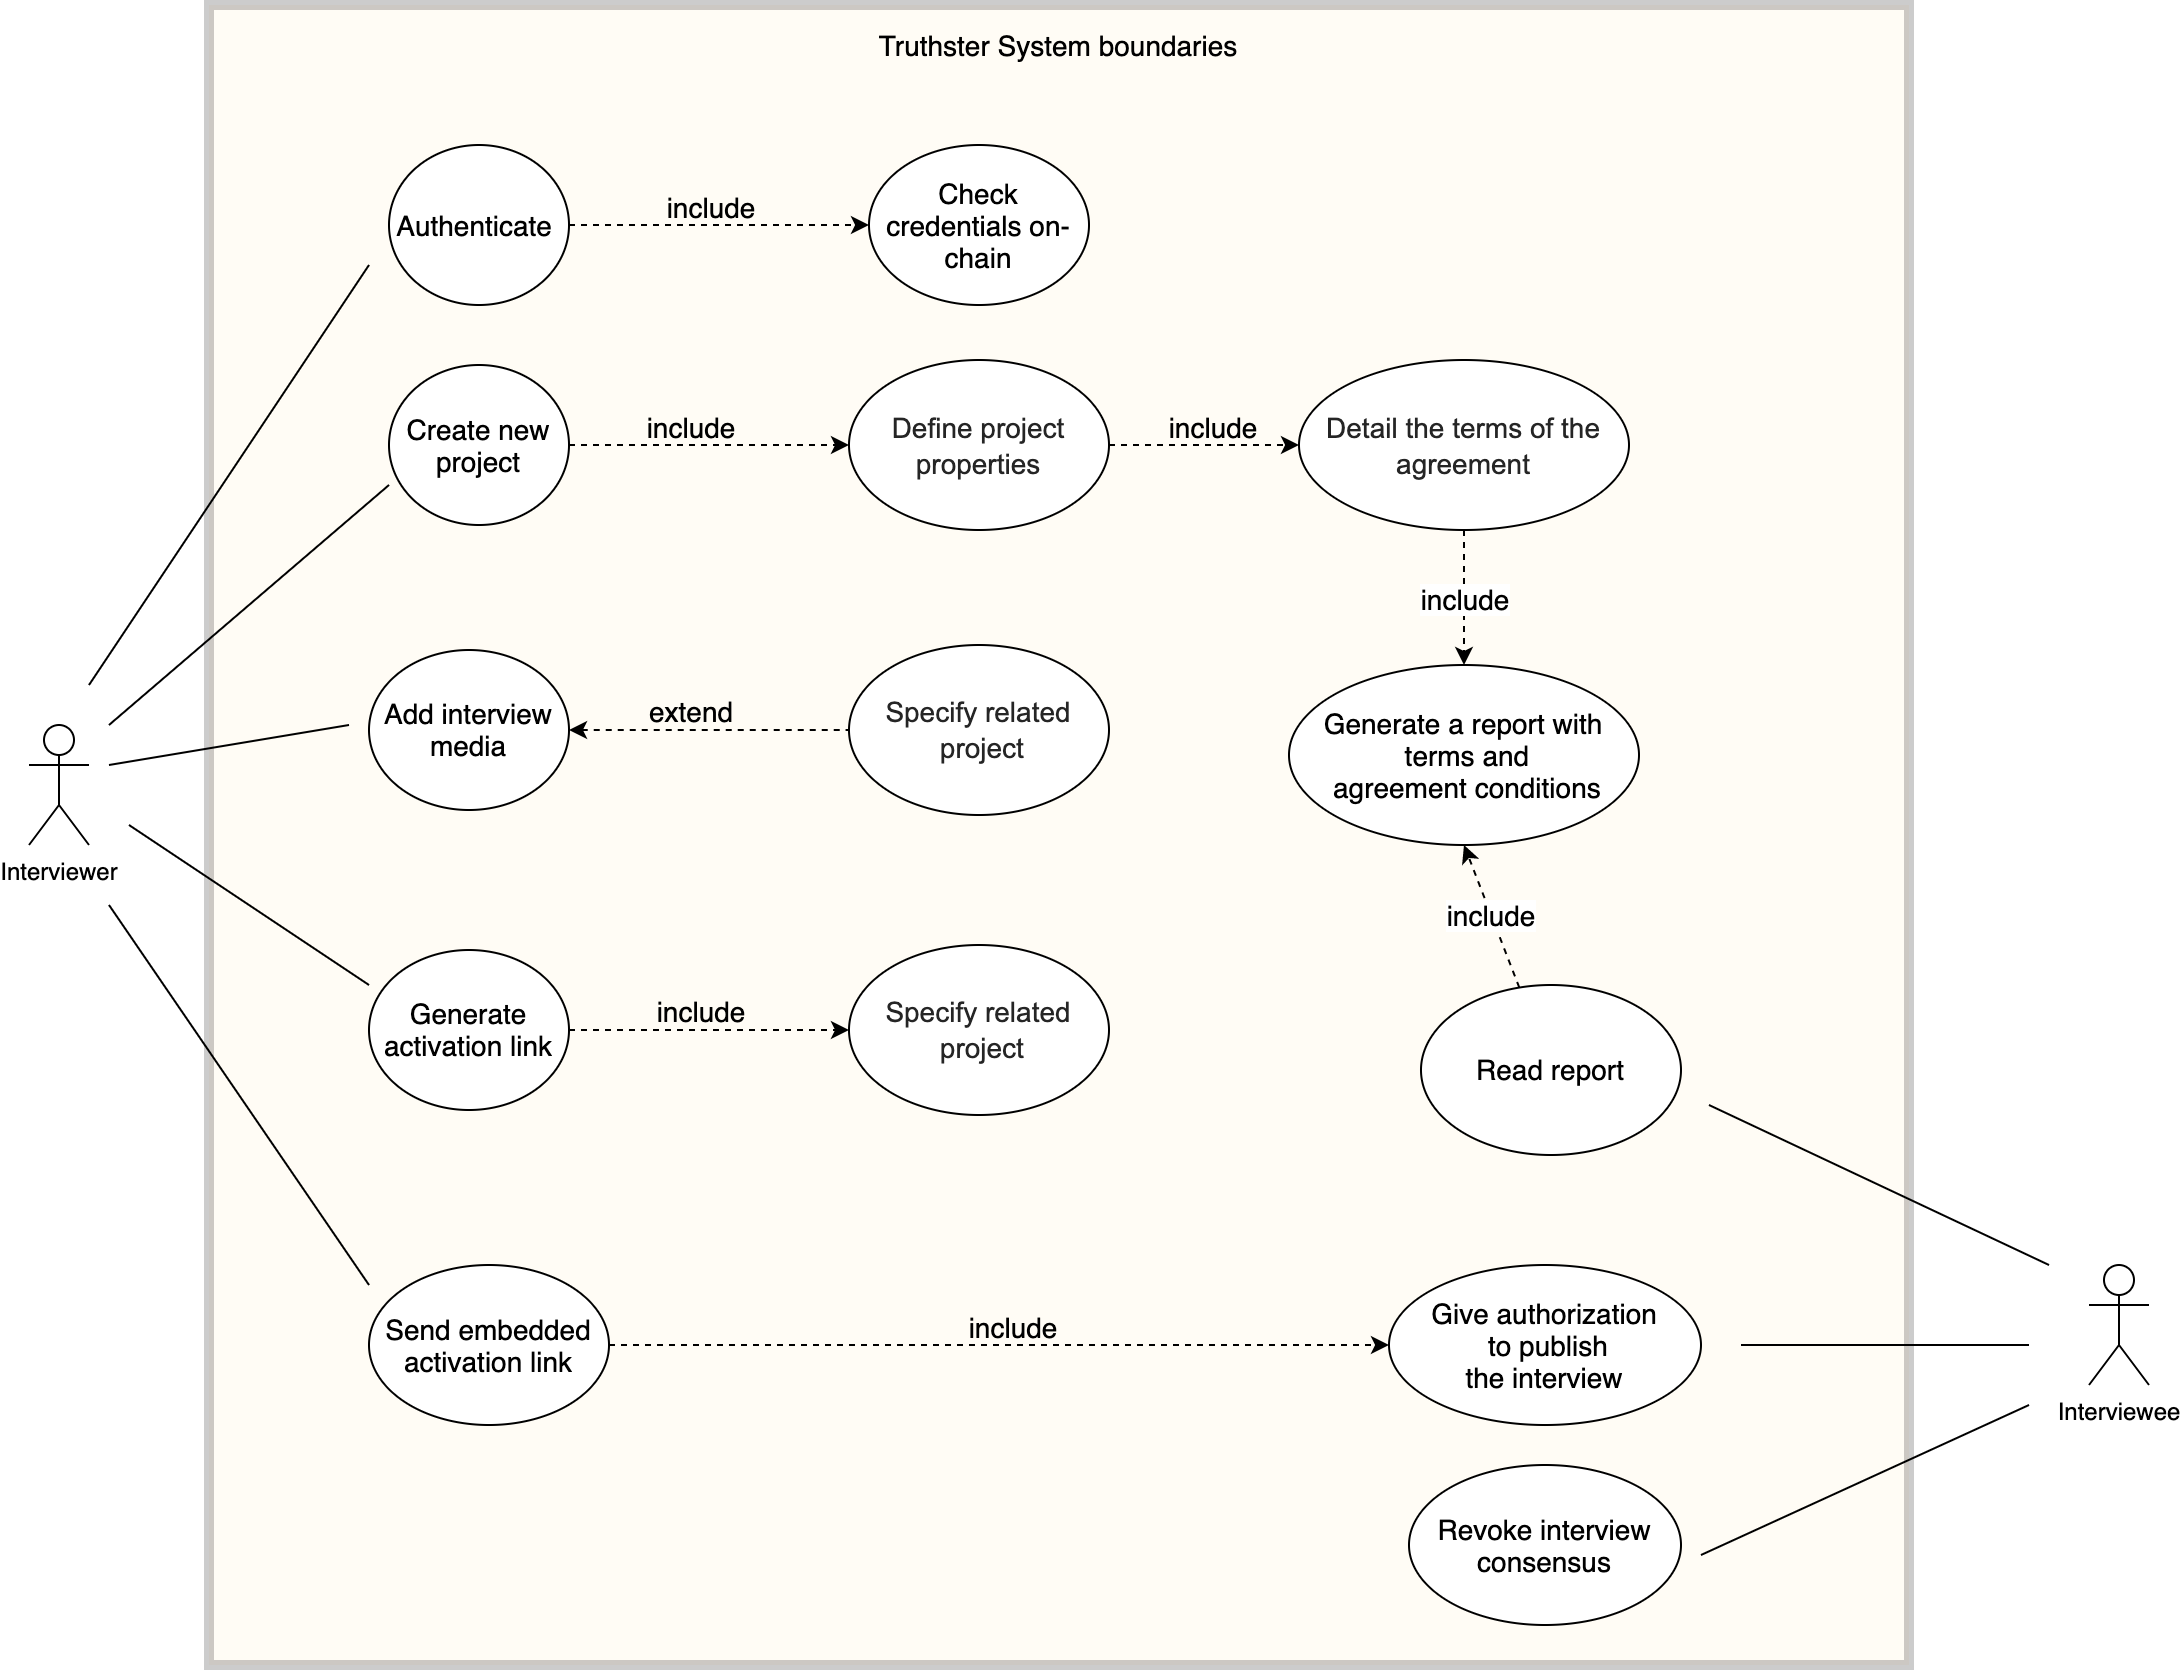
\includegraphics[width=0.8\textwidth]{images/truthster_use_cases.png}
    \caption{Truthster main use cases}
    \label{fig:useCaseDiagram}
\end{figure}

From the interviewer perspective we have:
\begin{itemize}
    \item \textbf{Authentication}: to ensure secure access to the Truthster platform, the system must authenticate the interviewer's identity before allowing them to use its features. This involves verifying the interviewer's credentials and checking their validity on-chain using blockchain technology. 
    \item \textbf{Create new project}: to create a new interview project on the Truthster platform, an interviewer must provide relevant information such as the interview date, related documents, and general project details, as well as the terms of the agreement with the interviewee. The Truthster system generates the agreement according to GDPR guidelines and ensures the privacy information is secure.
    \item \textbf{Add interview media}: once an interview is conducted on the Truthster platform, the output can be in the form of video, audio, or another format. To add this media to an existing project, the interviewer must be able to access the project and upload the media files to the system at a later stage.
    \item \textbf{Generate an activation link}: to ensure that the interviewee can access the interview media files and other relevant information associated with a specific project on the Truthster platform, the interviewer must be able to generate an activation link that refers to the project. This activation link is generated at the end of the interview and is sent to the interviewee to provide them with secure access to the relevant project. The interviewer can specify the project to which the activation link refers, ensuring that the interviewee can view the appropriate media files and information.
    \item \textbf{Send embedded activation link}: to ensure the interviewee can access the activation link generated for a specific project, Truthster must be able to send the activation link to the interviewee through different channels, including email, mobile message, or a QR code. By providing different methods of sending the activation link, the platform can cater to the different preferences of the interviewees and ensure that they can access the link securely and conveniently.
\end{itemize}

From the interviewee perspective we have:
\begin{itemize}
    \item \textbf{Read report}: once the interviewer generates a report regarding the terms and conditions of the interview through the Truthster platform, the interviewee must have a secure and user-friendly way to access and read the report.
    \item \textbf{Give authorization to publish the interview}: to ensure compliance with relevant regulations and protect the privacy of interviewees, Truthster must provide a secure and user-friendly way for the interviewee to give authorization for publishing the interview. The platform must enable the interviewee to provide their consent easily, while also providing them with all the necessary information and credentials to make an informed decision.
    \item \textbf{Revoke interview consensus}: to comply with relevant regulations and ensure privacy protection, Truthster must provide a secure and user-friendly way for the interviewee to revoke their consent to publish the interview.
\end{itemize}

\section{Functional requirements}

After conducting a thorough analysis of the existing challenges, we are now able to compile a comprehensive list of functional requirements that must be met by the Truthster system, in order to facilitate effective collaboration between interviewers and interviewees, while ensuring strict compliance with all relevant regulations and security protocols. These functional requirements are essential to address the identified issues and ensure the successful implementation of the Truthster system, providing a secure and reliable platform for all parties involved in the interview process.

\begin{itemize}

    \item \textbf{Verify interviewer identity}: ensuring the verification of an interviewer's identity before and after the interview is a crucial requirement for the Truthster system. Prior to the interview, it is important to authenticate the interviewer's credentials in order to ensure that only authorized personnel are granted access to the interviewee and any sensitive information involved in the interview process. This can help prevent unauthorized access or security breaches, and ensure that all parties can trust the integrity and authenticity of the system. Additionally, verifying the identity of the interviewer after the interview can help with any potential legal disputes or issues that may arise.
    \item \textbf{Certify and verify digital media with blockchain (Alastria)}: in order to ensure the authenticity and integrity of the digital media used in the Truthster system, it is important for the system to provide a way to certify and verify the media through the use of blockchain technology. This is where the Alastria blockchain platform comes into play. By leveraging the features of Alastria, Truthster can provide a secure and tamper-proof way of storing and verifying digital media, such as video interviews and user terms and agreement conditions documents. This not only helps to protect the privacy and security of the data, but also provides a way to build trust between the parties involved in the interview process.
    \item \textbf{Embed authorship and legal details}: embedding authorship and legal details into the digital media is an important functional requirement for the Truthster system. This ensures that authorship and legal aspects, such as portrayal and data protection consent, are properly recorded and cannot be manipulated. By embedding such details into the digital media, Truthster can help ensure the authenticity and integrity of the media and protect the rights of both the interviewer and interviewee. Additionally, embedding legal details into the digital media can aid in resolving potential legal issues by providing a clear record of consent and authorization. Thus, this requirement is critical in ensuring the reliability and legal compliance of the Truthster system.
    \item \textbf{Automate generation of legal terms}: in order to ensure compliance with legal regulations, Truthster must automate the generation of legal terms and conditions under which the content can circulate and be used. This functionality will help interviewers to create the required legal documentation and provide interviewees with the necessary information about how their content will be used. The system must be able to generate legally compliant documents that are specific to each project, taking into account the applicable regulations in each jurisdiction.
    \item \textbf{Easy certification tool for video interviews}: in order to facilitate the certification process for media content, Truthster should provide an easy-to-use tool that is focused on video interviews. The tool should be intuitive and accessible for all users, regardless of technical expertise, to ensure that the certification process can be completed efficiently and effectively. Additionally, the tool should be designed with the user in mind, providing clear guidance and feedback throughout the certification process to ensure that the resulting certification accurately reflects the authenticity and integrity of the media content.
    \item \textbf{Secure and manage interview data}: to ensure the confidentiality and security of all interview-related data, Truthster must store this information in a server that is encrypted and accessible only to authorized users. In addition, the data must be organized in a way that associates it with a specific project to facilitate its retrieval and management. This includes all media content, such as video interviews, and any relevant legal documents, user terms, and agreement conditions. To optimize data management and accessibility, the information should be stored in a database or server archive that can be easily searched, sorted, and updated. By implementing these measures, Truthster can ensure that its users' information is protected and easily accessible as needed.
    \item \textbf{Provide an identity verification tool}: Truthster must provide an easy-to-use tool for identity verification that can be used for a wide range of purposes beyond the interview process. This tool can be used for public authority identity checks, restricted area entry, or for revoking interviewee consent, among other applications. The system must be able to verify the identity of the user to ensure the security and privacy of all parties involved.
    
\end{itemize}

\section{Non-functional requirements}

The Truthster system aims to provide a secure and efficient solution for the verification and certification of digital media. In order to achieve this goal, it must meet a number of non-functional requirements that ensure its reliability, scalability, and user-friendliness. The following is a list of non-functional requirements for the Truthster system:\\

\begin{itemize}

    \item \textbf{High performance and scalability}: in order for the Truthster system to be effective and efficient, it is very important that it is designed to handle a high volume of concurrent users and large amounts of data without experiencing significant lag or downtime. This is especially important given the sensitive nature of the data that will be stored and managed by the system. To ensure optimal performance, the system must be designed with scalability in mind. This means that it should be able to adapt to changing user demands and accommodate increased traffic and data volume without impacting performance. In addition, the system should be able to distribute the load of data processing and storage across multiple servers or nodes, to avoid overloading any one component of the system. It is also important that the system is designed with robust error-handling and fault-tolerance mechanisms, to ensure that any potential failures or issues are quickly identified and addressed. Finally, regular performance testing and monitoring should be conducted to identify any potential bottlenecks or areas for improvement, to ensure that the system is always operating at peak efficiency. By focusing on performance and scalability, Truthster can ensure that its users have a seamless and reliable experience, while also maintaining the integrity and security of the data managed by the system.
    \item \textbf{Usability}: is a critical aspect of the Truthster system, as it must be accessible and easy to use for both interviewers and interviewees. The system should be designed with a user-centric approach, placing the user at the center of the design process to ensure that their needs and preferences are taken into consideration. Clear and concise instructions should be provided to guide users through the various processes and tasks required to use the system, and the interface should be intuitive and easy to navigate. This means that the system should be designed with a logical and consistent layout, with familiar and recognizable symbols and icons, and a clear hierarchy of information. To enhance usability, the system should also offer a range of options for customization and personalization, allowing users to tailor the interface to their individual preferences. Additionally, the system should be responsive and adaptable, able to adjust to the needs of different users and situations, and should provide clear and immediate feedback to users throughout the process. Usability testing should be conducted regularly to identify any potential issues or areas for improvement, and user feedback should be actively solicited and incorporated into the design process.
    \item \textbf{Security}: ensuring the security of the data managed by the Truthster system is fundamental to protecting the privacy and rights of both the interviewers and interviewees. To achieve this, the system must employ a range of security measures to ensure the confidentiality and integrity of all data stored and transmitted. This includes the use of encryption to protect all data in transit and at rest, as well as multi-factor authentication to verify the identity of all users. The system must also be designed with access controls and permissions to ensure that only authorized individuals have access to the data, and that access is restricted based on the specific roles and responsibilities of each user. In addition, regular security audits and testing should be conducted to identify and address any potential vulnerabilities or threats to the system. The system must also have measures in place to ensure the integrity of the media files, including the use of digital signatures and hashes to verify that the media has not been tampered with or altered in any way.
    \item \textbf{Compliance}: is a key factor for any system that handles sensitive data, and Truthster is no exception. The system must comply with all relevant laws and regulations, including the General Data Protection Regulation (GDPR) and copyright laws, to ensure that the privacy and rights of all parties involved are respected and protected. This means that the system must be designed to collect, store, and manage data in a way that meets GDPR requirements, such as obtaining consent from interviewees for the collection and processing of their personal data. Additionally, the system must comply with copyright laws to ensure that all media content used and stored by the system is legally obtained and used with proper authorization. To ensure ongoing compliance, the system must be regularly reviewed and updated to reflect any changes in relevant laws or regulations. The compliance team should work closely with legal experts to ensure that the system is designed and operated in accordance with all applicable laws and regulations, and to identify any potential risks or issues.
    \item \textbf{Interoperability} is a crucial aspect of modern software solutions, and Truthster is no exception. The system must be designed in a way that allows it to seamlessly integrate with other software solutions, platforms, and technologies. This will not only lead to a wider adoption of the Truthster system, but also allow other companies to easily become part of the platform and use its various services, such as authentication, verification, certification, and more.

\end{itemize}

After outlining the various use cases for Truthster and identifying the functional and non-functional requirements necessary for the system, the next step is to dive into the solution design. In the upcoming chapter, we will delve into the technical details of the system, exploring different available tools that can be utilized to build a robust and reliable platform. The solution design will take into consideration the previously outlined requirements and use cases, ensuring that the resulting system will be able to handle the desired functionality while meeting the necessary standards for usability, performance, security, and compliance. Additionally, the chapter will cover the various pros and cons associated with each tool or technology being considered, providing an in-depth analysis of the different options available to the project team. By examining these various factors and making informed decisions about the technical design, the project team can ensure that the resulting Truthster system will be a powerful and effective tool for managing and certifying media content.








\chapter{Solution design}
\label{chapter:solutionDesign}

After conducting a thorough analysis of the current state of the art in the field, we have designed a Truthster possible system solution that includes a mobile/web app, a back-end module, a blockchain node, and a database service (Figure~\ref{fig:truthsterArchitecture}). The mobile/web app serves as the primary user interface, allowing users to manage their projects and media. The back-end module, implemented in Node.js, handles the communications between the mobile app, blockchain node, and database via REST APIs, ensuring seamless integration between these components. The blockchain node, based on Alastria technology, provides secure access to the blockchain infrastructure, ensuring data integrity and authentication. The database service, implemented using MongoDB, serves as the primary storage mechanism for all interview-related data. In a later stage of development, we plan to include an additional SQL database to store data about interviewers and interviewees.\par
In the upcoming sections, we will provide a detailed analysis of the design choices we made for each component of the Truthster system.

\begin{itemize}

    \item \textbf{The front-end} of the Truthster system, a mobile/web app, is responsible for providing a user-friendly interface for the interviewer and interviewee to interact with the system. This includes functions such as recording audio and video material, inputting interview information and contact details, and selecting interview media. The front-end also handles authentication of the interviewer to ensure that only authorized personnel have access to the system.
    \item \textbf{The back-end} of the Truthster system acts as the central hub for all data and communication between the front-end and external services such as the Alastria blockchain and storage service. It receives and processes data from the front-end, including interview media and metadata, and communicates with the external services to securely store and verify the data. The back-end also handles notifications and archiving of past interviews on the interviewer's mobile app.
    \item \textbf{The Alastria blockchain} is a key component of the Truthster system, providing a decentralized platform for storing and verifying the authenticity and integrity of media files. The blockchain creates a tamper-proof record of the hashes of the media files, which can be used to provide proof of validity in legal proceedings. The blockchain also provides a way to securely store and manage personal data and consent agreements, in compliance with GDPR regulations.
    \item \textbf{The storage service} is responsible for storing the interview media files, metadata, and GPS positions of the interviewer and interviewee. It ensures that all data is securely stored and encrypted, and provides a way to easily search and retrieve interview data as needed. The storage service also supports backup and disaster recovery, ensuring that interview data is not lost in the event of a system failure or data loss.

\end{itemize}

Overall, these four components work together to provide a secure, reliable, and user-friendly platform for conducting and verifying interviews. The combination of front-end, back-end, blockchain, and storage service provides a complete solution that meets the functional and non-functional requirements of the Truthster system.

\begin{figure}
    \centering
    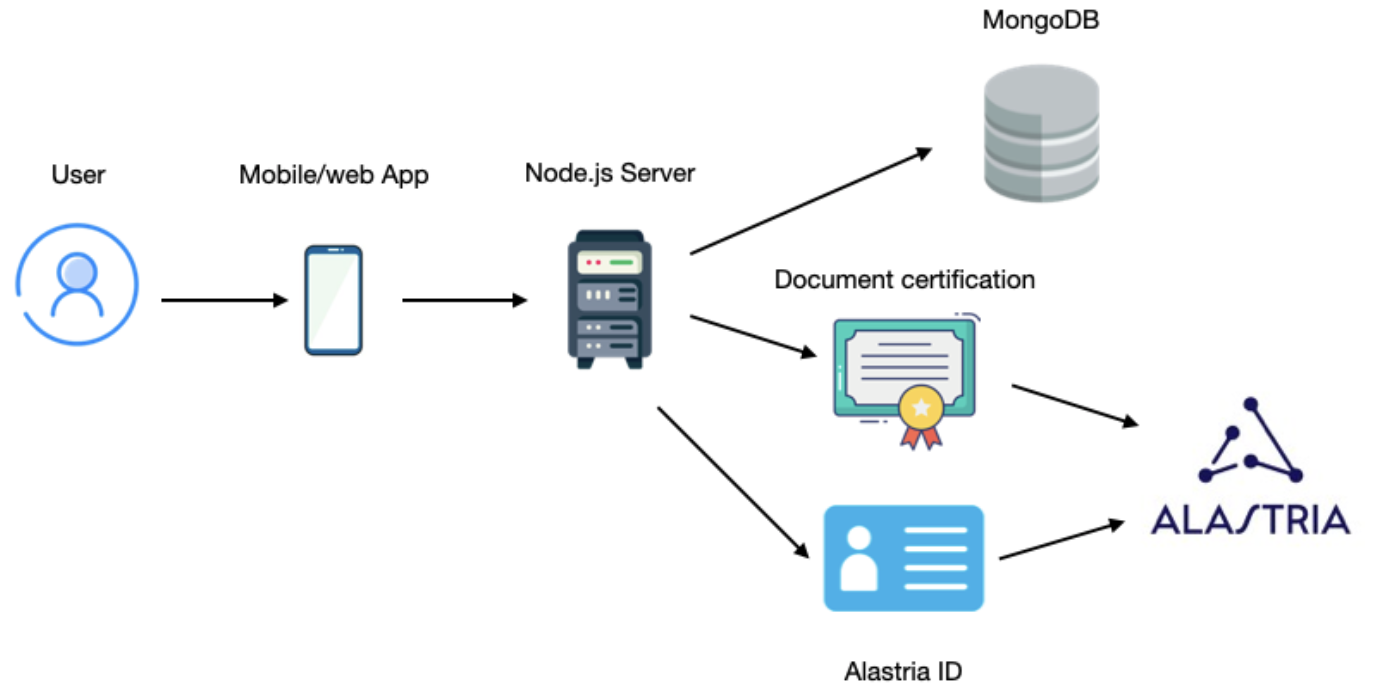
\includegraphics[width=0.8\textwidth]{images/technicalArchitectureStructuralView.png}
    \caption{Truthster system architecture}
    \label{fig:truthsterArchitecture}
\end{figure}


\section{Front-end}

The user interface (UI) of a system is a fundamental component that plays a significant role in the overall success and adoption of the software application by journalists and their audience. When designing the UI of a system, it is important to consider the available options and make an informed decision that meets the specific needs of the project.\par
In the case of the Truthster system, the chosen UI technology is a mobile/web app that allows users to manage their projects and media with ease. This type of implementation provides several advantages and disadvantages that should be considered when making the final decision.

Pros:

\begin{enumerate}

    \item \textbf{Accessibility}: one of the most significant advantages of a mobile/web app UI is that it can be accessed from anywhere and at any time, making it highly convenient for users to access the platform features.
    \item \textbf{User-friendly}: the mobile/web app UI is designed to be intuitive and easy to navigate, which makes it easy for users to use the platform features without requiring any technical knowledge.
    \item \textbf{Easy updates}: updating a mobile/web app UI is much simpler and quicker than traditional software updates, which means that any changes or improvements can be implemented quickly and easily adopting an agile development methodology.
    \item \textbf{Speed}: mobile/web app user interfaces (UIs) can offer a fast and responsive user experience as the processing is handled on the client-side, allowing for immediate user feedback and reducing the need for time-consuming server requests.

\end{enumerate}

Cons:

\begin{enumerate}
    
    \item \textbf{Limited functionality}: a mobile/web app UI is limited by the capabilities of the devices they run on, which means they may not be able to provide the same functionality as a desktop application.
    \item \textbf{Screen size}: the limited screen size of mobile devices can be a disadvantage for some users who may need more detailed information.
    \item \textbf{Compatibility}: the mobile/web app UI must be compatible with a wide range of devices and operating systems, which can be challenging and time-consuming to maintain.
    \item \textbf{Security}: mobile/web app UIs can be more susceptible to security vulnerabilities and attacks, which requires additional security measures to be implemented to ensure user data is secure.

\end{enumerate}

In conclusion, the mobile/web app UI is a suitable choice for the Truthster system, as it provides a convenient, user-friendly, and responsive user experience having downsides that are not much impacful on our design solution.

\section{Storaging service}

The classic solution for providing a storage service with a database is to use a relational database management system (RDBMS \cite{RDBMS}). An RDBMS is a type of database management system that is based on the relational model, which organizes data into one or more tables, with a unique key identifying each row. RDBMSs are popular because they provide a powerful and flexible way to store and manage data, with a wide range of features and capabilities. Some popular examples of RDBMSs include MySQL \cite{mySQL}, Oracle \cite{oracleDb}, Microsoft SQL Server \cite{microsoftSQL}, and PostgreSQL \cite{postgreSQL}. These databases are widely used in a variety of applications and industries, ranging from small-scale web applications to large-scale enterprise systems. One advantage of using an RDBMS is that they provide strong data integrity, with the ability to enforce complex relationships and constraints between tables. However, they can be complex to set up and maintain, and may not be well-suited for handling large volumes of unstructured or non-relational data.\par
Now let's shift our focus to NoSQL databases, which provide a different approach to data storage compared to traditional relational databases. NoSQL databases are a type of non-relational database that provide a flexible and scalable alternative to traditional SQL databases. Unlike SQL databases, NoSQL databases are designed to handle large amounts of unstructured or semi-structured data, making them well-suited for use cases such as web applications, mobile applications, and big data analytics. This type of databases can store data in various formats, such as document-oriented, key-value, column-family, and graph databases and this allows for a high degree of flexibility in data modeling, making it easier to adapt to changing business requirements. Additionally, NoSQL databases can provide high availability and scalability by distributing data across multiple nodes, making them an ideal choice for applications that require high performance and reliability. Some of the most popular NoSQL databases include MongoDB \cite{mongoDB}, Cassandra \cite{cassandra}, Redis \cite{redis}, and CouchDB \cite{apacheCouch}.\par
In designing the data storage component for the Truthster system, a decision was made to adopt a NoSQL database as the primary storage solution. MongoDB was chosen due to its scalability and flexibility in handling data with varying structures, which is a key requirement of the system given that the data collected during interviews may come in different formats. The use of a NoSQL database like MongoDB also allows for faster data retrieval and processing due to its ability to horizontally scale out to multiple nodes. While a NoSQL database is the primary choice, it is important to note that a relational database may be needed in the future to store additional data about interviewers and interviewees. As such, plans have been made to incorporate a relational option in future developments of the system to complement the NoSQL database. This hybrid approach to data storage will ensure that the system can handle both structured and unstructured data, while also maintaining scalability, flexibility, and maintainability.

\section{Back-end}

The Truthster system is a comprehensive platform that has been thoughtfully designed with a classic three-tier architecture \cite{3tierArchitecture} solution in mind. This architecture utilizes a server-side application that processes requests from the client-side and interacts with the database to provide centralized control and management of the application. The back-end of the system is the central actor in this architecture, managing communication between the front-end, the database (MongoDB), and Alastria blockchain. By using RESTful APIs \cite{restAPI}, the Truthster system can facilitate communication between the different components of the architecture in a secure and efficient manner. The use of JWT tokens \cite{jwtTokens} and AlastriaID further ensures that only authorized users can access sensitive data and services within the system.\par
In any software application, the back-end system plays a crucial role in determining its reliability, scalability, and performance. For the Truthster system, the decision was made to implement the back-end using a Node.js server \cite{nodeJs}. Node.js is an open-source platform that has gained immense popularity for its ability to build scalable, high-performance applications. Its ability to handle a large number of connections with low overhead makes it an ideal choice for applications that require high scalability. Additionally, Node.js has a large and active developer community, providing a wealth of support and resources for future feature additions and updates.\par
The use of Node.js for the back-end of the Truthster system ensures a robust and scalable system for managing data, communication, and authentication. Node.js is scalable, reliable, and offers a wide range of libraries that can be easily integrated into the Truthster system. By leveraging these libraries, the development team can quickly add new features and functionality to the system without the need to write code from scratch. The focus on building the core functionality of the system allows the Truthster team to deliver a reliable and feature-rich user experience in a timely manner. Node.js and its vast library ecosystem make the Truthster back-end system well-positioned to adapt and grow with the needs of the platform and its users.\par
In conclusion, the use of Node.js and its libraries makes the Truthster system more scalable, reliable, and feature-rich. By utilizing a classic three-tier architecture, RESTful APIs, JWT tokens, and AlastriaID, the Truthster system ensures secure and efficient communication between different components of the architecture. The use of Node.js for the back-end of the system provides the necessary scalability and performance for a successful platform. With the wide range of libraries available, the Truthster team can quickly add new features and functionality to the system in response to the needs of the platform and its users. Overall, the choice of technologies and architecture for the Truthster system provides a robust and scalable platform that can adapt and grow with the needs of its users.

\section{Alastria blockchain}

Blockchain technology has become increasingly popular in recent years due to its security, immutability, and decentralized nature. For the Truthster system, we have chosen to connect our back-end to a node of the Alastria blockchain \cite{alastriaBlockchain}. By connecting to an Alastria node, we gain access to the entire blockchain ecosystem, including smart contracts that are already deployed on the network.\par
Alastria is a permissioned blockchain that provides a range of services to its users, including identity and access management, decentralized storage, and smart contract functionality. In the context of Truthster, we plan to leverage the benefits of Alastria blockchain to provide secure and immutable data storage, as well as ensure the confidentiality and integrity of user data. In the upcoming Alastria chapter, we will explore the benefits and potential of Alastria blockchain in more detail and how it can be leveraged to build a secure and scalable system for Truthster.




\chapter{AlastriaID: a DLT-based digital identity}
\label{chapter:alastriaID}


AlastriaID is a digital identity project by the Identity Commission of Alastria. It aims to provide a legal and technical framework for sovereign digital identity projects in the Eurozone, following the guidelines of the EIDAS Regulation and the e-Identity Workshop Report of the EU Blockchain Observatory and Forum. The AlastriaID model is designed to work with the Alastria Standards Commission to standardize processes and methodologies and is designed to be complementary with the General Data Protection Regulation (GDPR).\par
From a more technical perspective AlastriaID is a decentralized identity framework that allows users to securely store and manage their personal information in a decentralized environment. The framework is based on a set of smart contracts, that have been written in Solidity allowing to deploy them on any EVM compatible blockchain, and JWT (JSON Web Tokens), which are compact and self-contained data structures used for transmitting information between parties. 

\subsection{The roles in AlastriaID}

AlastriaID has three main entities where each one play a specific role in the framework: service providers, issuers, and subjects that interect in different ways in order to provide its services:

\begin{itemize}

    \item \textbf{Subjects}: in the AlastriaID model they are individuals or organizations that hold a digital identity on the platform. Subjects are the central entity in the AlastriaID ecosystem and have complete control over their personal data (Self-Sovereing Identity). The digital identity of a subject is stored on the blockchain and is tied to a unique identifier, allowing the subject to prove their identity in a secure and verifiable manner.\par
        Subjects can use their digital identity for a variety of purposes, including accessing online services, participating in online transactions, and securely sharing personal information with service providers. For example, a subject can use their digital identity to open a bank account, apply for a loan, or access government services online. The subject's digital identity can also be used to prove their identity in other possible scenarios, such as when voting in an election or accessing secure facilities (despite this hasn't been done yet, it can be a nice field to apply blockchain technology in the next future).
        Subjects have full control over their personal data and can choose to share it with service providers as needed. They can also revoke access to their personal data at any time, ensuring that their data remains secure and under their control. This is a significant advantage over traditional identity systems, where personal data is often stored in centralized databases that are vulnerable to data breaches and other security risks.

    \item \textbf{Service Providers}: in the AlastriaID model they are organizations that provide various services to subjects using the platform. They are able to request and receive specific information from subjects to provide these services, ensuring that personal data is protected and under the control of the subject at all times. Service providers can provide a wide range of services to subjects, including financial services, healthcare services, and government services. For example, a healthcare service provider may request and receive medical information from a subject to provide personalized care, while a financial service provider may request and receive financial information from a subject to provide a loan.
        Service providers can use the AlastriaID platform to access a secure and verifiable digital identity for each subject, ensuring that personal information is protected and that the subject's identity can be trusted. This is in contrast to traditional service providers, who often rely on centralized databases that are vulnerable to data breaches and other security risks.
        In addition to providing services to subjects, service providers can also act as verifiers, helping to ensure that digital identities are secure and can be trusted across the AlastriaID ecosystem. This helps to create a decentralized and interoperable ecosystem for digital identities that can be used across a wide range of applications and services.

    \item \textbf{Issuers}: in the AlastriaID model they are organizations that are authorized to issue digital identities to individuals and organizations on the platform. They play a critical role in the AlastriaID ecosystem by verifying the identity of subjects and issuing a secure and verifiable digital identity. Issuers are responsible for verifying the identity of a subject through a process known as "know your customer" (KYC). This involves collecting and verifying personal information about the subject, such as their name, address, and government-issued identification. Once the identity of a subject has been verified, the issuer can issue a digital identity to the subject that is stored on the blockchain in some way.
        Examples of issuers in the AlastriaID ecosystem include banks, government agencies, and telecommunications companies. For example, a bank may act as an issuer and verify the identity of a subject when they open a new bank account. The bank would then issue a digital identity to the subject that can be used for other financial services, such as applying for a loan or accessing government services. In addition to verifying the identity of subjects, issuers can also act as verifiers, providing a secure and reliable infrastructure for the storage and management of digital identities. This ensures that digital identities are secure and can be trusted across the AlastriaID ecosystem.
        
\end{itemize}

In the AlastriaID framework, service providers can request and verify digital credentials from subjects, while issuers can issue and manage the digital credentials. The system is designed to provide a secure and decentralized environment for the management and control of personal information.

\subsection{GDPR and Decentralized IDentifier}
The General Data Protection Regulation (GDPR) is a crucial component of the AlastriaID model as it governs the protection and management of personal data, ensuring that the privacy rights of subjects are respected and upheld.
AlastriaID can help organizations comply with the General Data Protection Regulation (GDPR) by providing a secure and privacy-preserving infrastructure for managing personal data.\par
With AlastriaID, organizations can:

\begin{itemize}

    \item \textbf{Store personal data securely}: AlastriaID uses blockchain technology to secure personal data, making it tamper-proof and reducing the risk of data breaches. Specifically, the framework store the hash of the actions undertaken with this framework acting as a tracker to verify information on-demand.
    \item \textbf{Control access to personal data}: AlastriaID allows organizations to control who has access to personal data, ensuring that only authorized parties can access it.
    \item \textbf{Track data usage}: AlastriaID provides a clear audit trail of all data usage, allowing organizations to track who has accessed personal data and when. This helps organizations meet the GDPR's requirements for data transparency and accountability.
    \item \textbf{Provide data portability}: AlastriaID enables individuals to easily and securely transfer their personal data from one organization to another, helping organizations meet the GDPR's requirements for data portability.
    \item Overall, AlastriaID can \textbf{help organizations comply with the GDPR} by providing a secure, privacy-preserving, and transparent infrastructure for managing personal data (credentials can be revoked by users or expire because of a time limitation). By doing so, organizations can reduce the risk of data breaches, improve data security, and ensure that they are meeting their obligations under the GDPR.

\end{itemize}

In order to offer all of its features AlastriaID leverages the concept of \textbf{Decentralized IDentifier (DID \cite{DID})}.

Decentralized Identifiers (DIDs) are a new type of globally unique identifier that are designed to enable individuals and organizations to generate their own identifiers using systems they trust. In contrast to traditional identifiers, DIDs are not issued by an external authority, but are instead generated and maintained by the entity that requires the identifier. This new type of identifier is becoming increasingly important in the Web3 as it provides a secure, entity-controlled mechanism for establishing identity and conducting verifiable transactions online.
In the current centralized web, our online identities are largely controlled by third-party entities such as social media platforms, email providers, and government institutions. This means that our online interactions are often tracked and monitored, and that we have limited control over the personal data we share online. DIDs provide a solution to these problems by enabling individuals and organizations to establish their own online identities that are controlled solely by them (here born the concept of Self Sovereing Identity \cite{selfSovereignIdentity}).
The use of DIDs enables users to create multiple identities that are each scoped to a specific context or interaction. For example, an individual might have a different DID for their personal life, their work life, and their hobbies. This provides users with greater control over their personal data, as they can choose to reveal only the information that is necessary for a given interaction. Additionally, because DIDs are generated and maintained by the entity that requires the identifier, there is no central authority that can revoke or deactivate the identifier.
In the web3, DIDs play a critical role in enabling secure, verifiable transactions and interactions indeed, a DID can be used to establish the identity of a user when conducting a secure financial transaction or when accessing a decentralized application like the one offer by the overall Truthster system for both journalists and people that uses their contents. Because the use of DIDs is built on strong cryptographic principles, users can trust that their online interactions are secure and that their personal data is protected.\par
Because of all the reasons just listed DIDs are a critical component of the web3, as they provide individuals and organizations with a secure, entity-controlled mechanism for establishing identity and conducting verifiable transactions online. The use of DIDs enables users to have greater control over their personal data and to interact online with confidence, knowing that their online identities are secure and verifiable.

With the implementation of DIDs inside the AlastriaID library, a wide range of applications and use cases become possible. The AlastriaID library provides a set of tools and APIs that enable developers to easily incorporate DIDs into their applications, making it possible to implement secure, verifiable transactions and data sharing. With DIDs, individuals and organizations can verify their identities, sign digital documents, give their consensus for contents that needs to be be published, and share personal data in a secure and controlled manner. Additionally, the AlastriaID library supports the creation of self-sovereign identities, enabling users to have full control over their personal data and the sharing of that data with others as previously described. These capabilities have the potential to revolutionize the way we interact and transact online, and the AlastriaID library is at the forefront of this change.\par
In the next sections we will go deeper in the implementation of the AlastriaID describing the main use cases that involve the library with its smart contracts and the DID implementation mechanisms.

\subsection{AlastriaID composition}

The AlastriaID framework is comprised of three open source libraries that provide the necessary components to develop and deploy decentralized digital identities on the AlastriaID platform.

\begin{itemize}

    \item The \textbf{alastria-identity-lib \cite{alastriaIdentityLib}} library provides developers with a set of reusable components written in Typescript that can be used to build and manage digital identities from a server and mobile side (its structure is represented in the Figure~\ref{fig:alastriaSCStructure}). This includes functions for creating, managing, and storing digital identities, as well as managing access to personal data through JWT tokens.
    \item The \textbf{alastriaID-truffle-contracts \cite{alastriaSmartContracts}} library provides developers with a set of smart contracts that can be used to deploy and manage digital identities on the Alastria blockchain. These contracts provide a Solidity implementation of a secure and verifiable infrastructure for storing and managing digital identities on any EVM compatible blockchain, and can be easily integrated into other applications and services to achieve a more complete usage of the framework.
    \item The \textbf{alastria-identity-example \cite{alastriaIdentityExample}} library provides developers with a sample implementation of the AlastriaID framework, demonstrating how the various components of the platform can be used to build and deploy decentralized digital identities. This library can be used as a starting point for building custom solutions and integrating AlastriaID into other applications and services like what we are going to do with Truthster.

\end{itemize}

Together, these libraries provide a comprehensive framework for developing and deploying decentralized digital identities on the AlastriaID platform. 
As we have just seen AlastriaID offers a range of features that allow users to securely manage and control their personal data in a decentralized manner. These features include: the ability to create and manage digital identities, control access to personal data, and provide a secure infrastructure for storing and managing digital identities. These features are designed to empower individuals and organizations to take control of their personal data and manage it in a secure and decentralized manner.\par
The following section will provide a more in-depth look at these key features of AlastriaID and how they work to provide users with a secure and verifiable digital identity.

\subsection{Alastria smart contracts structure}

The smart contracts used in the AlastriaID model are structured in Figure~\ref{fig:alastriaSCStructure}, where each arrow represents a dependency of the type "contract A uses contract B":

\begin{figure}
    \centering
    \includegraphics[width=0.8\textwidth]{images/alastriaSmartContractsStructure.png}
    \caption{Alastria smart contracts structure}
    \label{fig:alastriaSCStructure}
\end{figure}

The smart contracts act together in this schema and the major part of the actions are done through the AlastriaIdentityManager instance.\par
The following are lists of the key smart contracts used in the AlastriaID platform, each with its unique role and function.

\begin{table}[h!]
    \begin{tabular}{|p{6cm}|p{12cm}|}
    \hline
    Smart Contract & What is does\\ [0.5ex] 
    \hline\hline
    AlastriaIdentityManager.sol	 & It generates access tokens, creates identities, deploys an AlastriaProxy for each identity and sends transactions through the proxy of the sender\\ 
    \hline
    AlastriaProxy.sol & It is the Alastria ID itself. Only receives transactions from the IdentityManager and resends them to the target \\ 
    \hline
    AlastriaIdentityIssuer.sol & It keeps a registry of the issuers identities \\
    \hline
    AlastriaIdentityServiceProvider.sol & It keeps a registry of the service providers identities \\
    \hline
    AlastriaIdentityEntity.sol & It keeps a registry of the entities \\
    \hline
    \end{tabular}
    \caption{AlastriaID Smart contracts - Identity Manager}

\end{table}

\begin{table}[h!]
    \begin{tabular}{|p{6cm}|p{12cm}|}
    \hline
    Smart Contract & What is does\\ [0.5ex] 
    \hline\hline
    AlastriaCredentialRegistry.sol & It manages all the credentials and keeps the registry and the status\\ 
    \hline
    AlastriaPresentationRegistry.sol & It manages all the presentations and keeps the registry and the status\\
    \hline
    AlastriaPublicKeyRegistry.sol & It manages all the public keys and keeps the registry \\
    \hline
    \end{tabular}
    \caption{AlastriaID Smart contracts - Registry}

\end{table}

\begin{table}[h!]
    \begin{tabular}{|p{6cm}|p{12cm}|}
    \hline
    Smart Contract & What is does\\ [0.5ex] 
    \hline\hline
    EIDAS.sol & It manages EIDAS level of assurance for credentials \\ 
    \hline
    Owned.sol & It assures that just the account which deployed a contract can update the version \\ 
    \hline
    \end{tabular}
    \caption{AlastriaID Smart contracts - Libs}

\end{table}

\begin{table}[h!]
    \begin{tabular}{|p{6cm}|p{12cm}|}
    \hline
    Smart Contract & What is does\\ [0.5ex] 
    \hline\hline
    AlastriaNameService.sol	 & It creates the first entity to work with the rest of functionalities of Alastria Identity \\ 
    \hline
    \end{tabular}
    \caption{AlastriaID Smart contracts - Name Service}

\end{table}

\section{AlastriaID - Primary functions}

In this section, we will outline the primary functions that can be performed using the AlastriaID framework.
In particular we will explain how to:

\begin{enumerate}

    \item Create the \textbf{first entity} of the framework
    \item Create a brand new \textbf{AlastriaID}
    \item \textbf{Authenticate} with AlastriaID
    \item Create a \textbf{new entity}, upgrade its role (referring to the creation of a new issuer) and delete the added role
    \item Create new \textbf{credentials} for an entity
    \item Create a new \textbf{presentations} for an entity, update and check its status

\end{enumerate}

All of the above mentioned tasks involve a technical library that allows to store private and public key in special encrypted files: the keystores. This library called \textbf{keythereum} is available on Github \cite{keythereum}. Due to the large amount of boilerplate code involved in the library, we will handle it at a higher level. In some scenarios, such as when an actor signs a token or a transaction, it is essential to remember that this action demands the actor to load the keystore, decrypt it with their password, and retrieve the private/public key associated with it. Although this process will not be explicitly mentioned in the system, it is a vital step that must be undertaken by the actor to accomplish certain tasks within the framework.\par
In the upcoming sections, we will explore various scenarios that illustrate the functionality of the AlastriaID framework and how it can be leveraged within the Truthster system to accomplish tasks such as creating a new AlastriaID, managing credentials, and deleting roles. To make these scenarios more comprehensible, we will provide hypothetical role definitions, where the Truthster back-end will serve as both a service provider and issuer. We will also introduce a user named Bob, who will create a new AlastriaID, interact with the platform, and manage credentials and presentations. By using these "concrete" examples, we aim to provide a clearer understanding of how the AlastriaID framework can be utilized within the Truthster system.

\subsection{Create the first entity of the framework}

In AlastriaID, there is a first entity known as the root entity, which has the permission to create other entities within the platform. The root entity is created when the AlastriaID smart contracts are first deployed, in our framework through the AlastriaNameService contract. This root entity is responsible for creating other entities, such as subjects, service providers, and issuers, within the AlastriaID platform. The root entity is designed to provide a secure and centralized mechanism for managing entities within the platform, ensuring that only authorized entities have the ability to create and manage digital identities and personal data.

\subsection{Create an AlastriaID}

To create his AlastriaID, Bob contacts the Truthster backend and initiates the process. In response, the backend starts creating an Alastria Token (AT) that contains all the required information about Bob, such as his public key and Decentralized Identifier (DID). Once the AT is complete, Truthster signs it and sends it back to Bob. Bob then creates the transaction "createAlastriaID" and signs it, along with an Alastria Identity Creation (AIC) token. The AIC token contains the signed Alastria Token (sAT), Bob's public key, and the signed transaction, all of which are necessary for creating the AlastriaID. After signing the AIC, Bob sends it and the transaction bytecode to the Truthster backend for verification.\par
The Truthster backend then validates the received signed AIC (sAIC) using Bob's public key, and proceeds to create the transaction "prepareAlastriaID" to enable the platform to create a new AlastriaID. The backend signs this transaction before sending it to the Alastria network. Once the network has successfully processed the "prepareAlastriaID" transaction, the backend waits for its receipt and then sends the "createAlastriaID" transaction. Again, it waits for the receipt to confirm that the transaction was successful. Upon receiving the receipt, the backend sends a reading transaction to Alastria requesting the identity key of Bob's newly created AlastriaID. Alastria responds with the AlastriaID, which the Truthster backend then extracts and saves the associated proxy address. The backend creates the DID for Bob and sends it to him, which he saves locally for future use. In this way, the entire process of creating an AlastriaID is completed securely and accurately, with all necessary checks and validations being performed at each step of the process.
The process is represented in the Figure~\ref{fig:addAlastriaID}.

\begin{figure}
    \centering
    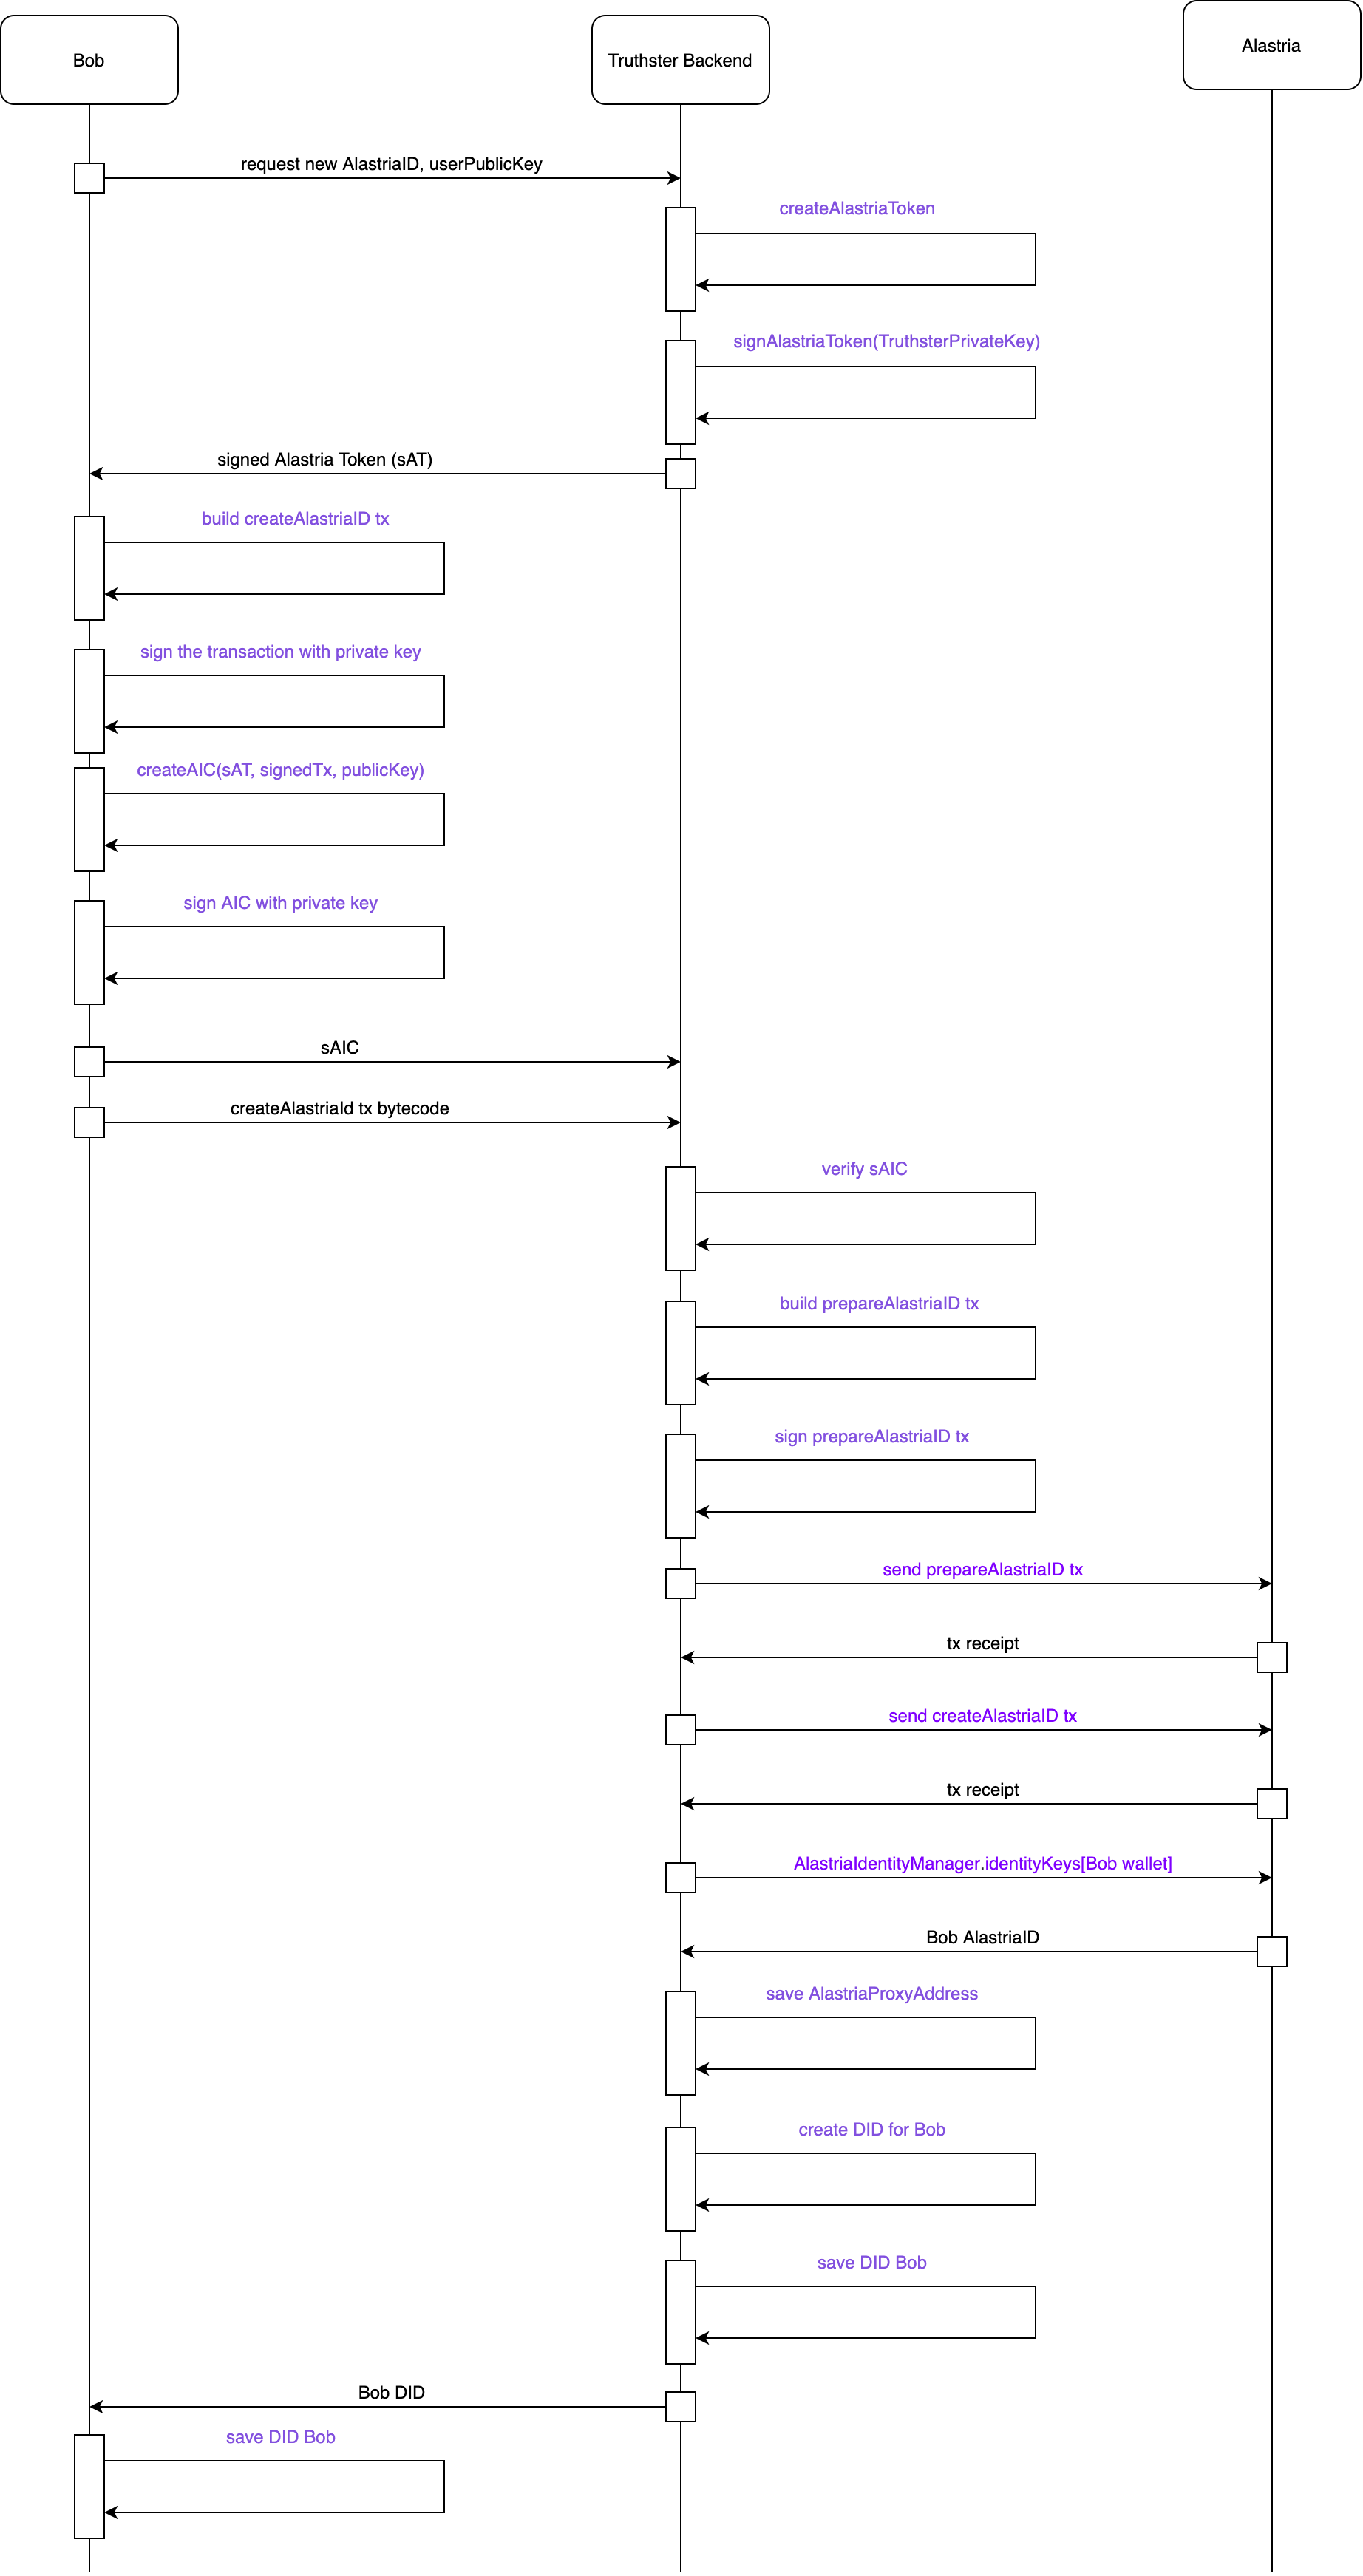
\includegraphics[width=0.8\textwidth]{images/createNewAlastriaID.png}
    \caption{Creation process for new AlastriaID}
    \label{fig:addAlastriaID}
\end{figure}

\subsection{Authentication with AlastriaID}

In Truthster, users can authenticate themselves on the system using a user-friendly app. This app allows users to easily create and manage their digital identities, as well as control access to their personal data.
When Bob wants to authenticate he sends to Truthster a login request. After receiving the request the Truthster backend generates an Alastria Token with all the information needed (expiring date, Truthster DID, etc...), signs and sends it back to the Bob. At this point Bob verify the authenticity of the AT with the Truhster public key. If everything is ok he procedes by creating an Alastria Session Token that is then signed with its private key and sent to the Truthster backend. After receiving the signed AST the backend verifies its authenticity with Bob public key and then if everything is fine the user is authenticated and can access the services provided by Truthster.

\begin{figure}
    \centering
    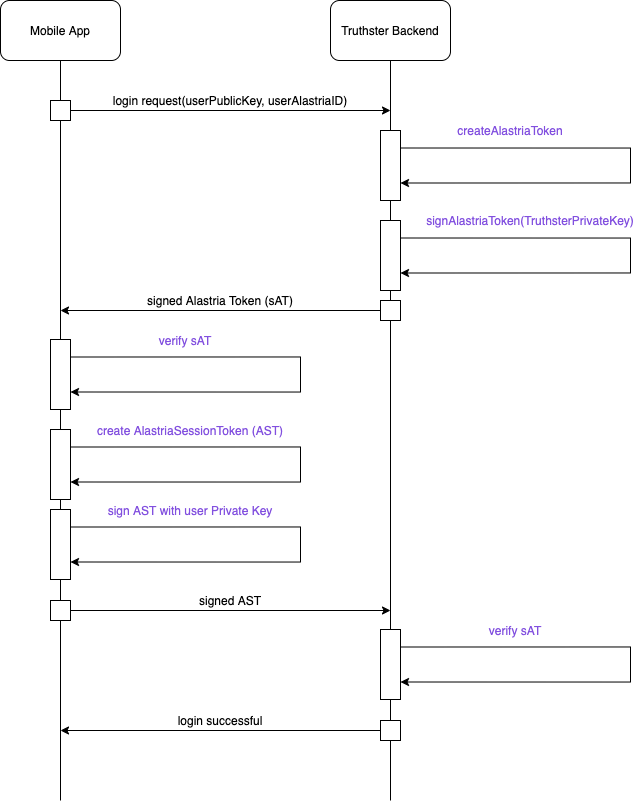
\includegraphics[width=0.8\textwidth]{images/authenticationAlastriaID.png}
    \caption{Authentication process with AlastriaID}
\end{figure}


\subsection{Create a new entity}

In order to create a new entity on the Alastria platform, the Truthster backend must first determine the role that this entity will play. By default, any new entity that is created will be classified as a Subject. However, if necessary, this entity can be upgraded to a Service Provider or Issuer through a transaction sent by another identity (it can be the first identity of the platform or an entity with a higher EIDAS level).
Once the role of the entity has been established, the Truthster backend builds the transaction "alastriaNameService.addEntity" which includes all the relevant information about the new entity. This information may include the entity's name, its AlastriaID, and any other necessary details. After assembling this information, the backend signs the transaction and sends it to the Alastria network for processing.
Alastria then performs the necessary checks and validations to ensure that the transaction is valid and that the new entity can be added to the platform. If the transaction is successful, Alastria sends a transaction receipt back to the Truthster backend, indicating that the entity has been successfully added to the platform.
The process is represented in the Figure~\ref{fig:createNewGeneralEntity}.\par
\textit{Notes}: when we create a new entity the subject of this operation must already have an AlastriaID since create the entity is a further step in the platform processes.

\begin{figure}
    \centering
    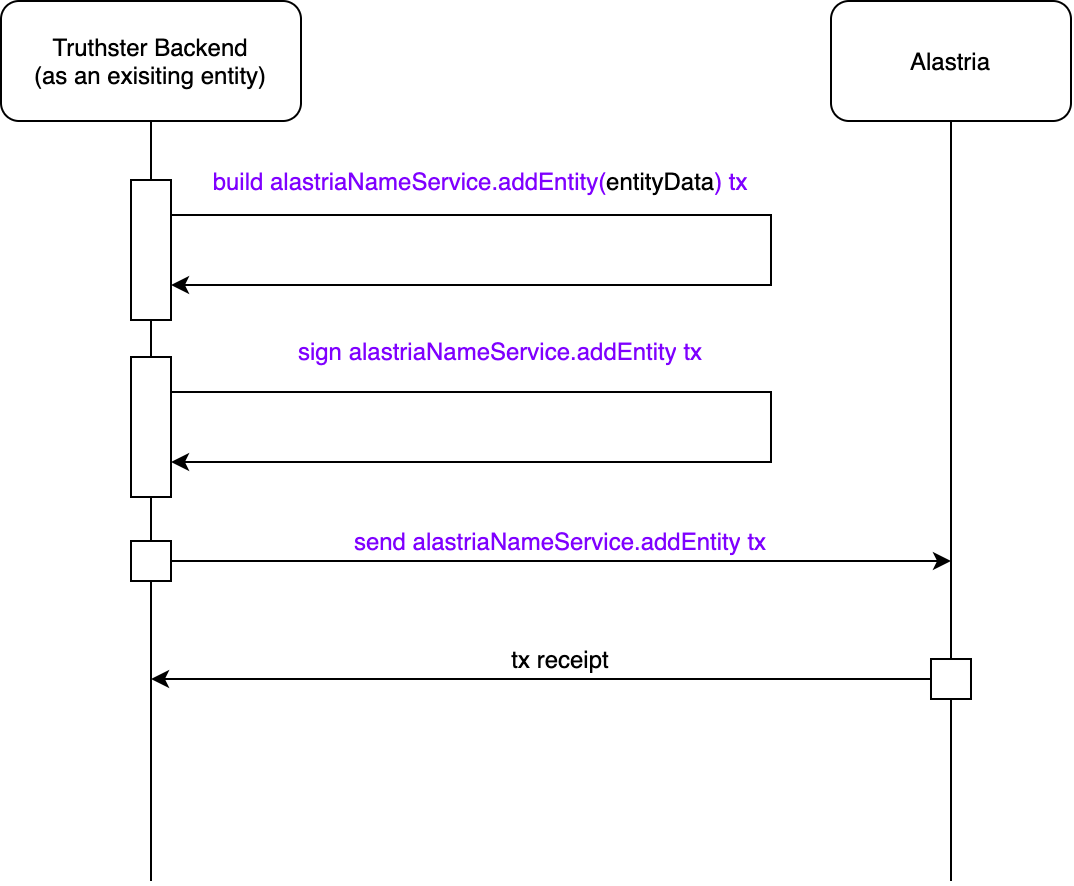
\includegraphics[width=0.8\textwidth]{images/createNewGeneralEntity.png}
    \caption{Creation process for new entities on-chain}
    \label{fig:createNewGeneralEntity}
\end{figure}

\subsection{Add new issuer}

To create a new issuer on the AlastriaID platform, the Truthster backend, which is itself an issuer and has the ability to create other issuers, must perform a series of steps. First, it creates a transaction called "identityManager.addIdentityIssuer," which includes the DID of the new issuer to be created and its EIDAS level as parameters. Next, the Truthster backend signs the transaction and sends it to Alastria. The transaction is then executed, and the Truthster backend receives the transaction receipt as confirmation. Ultimately, this process allows the creation of a new issuer on the Alastria blockchain platform, facilitated by the Truthster backend as the initial issuer and transaction creator.
The process is represented in the Figure~\ref{fig:addNewIssuer}

\begin{figure}
    \centering
    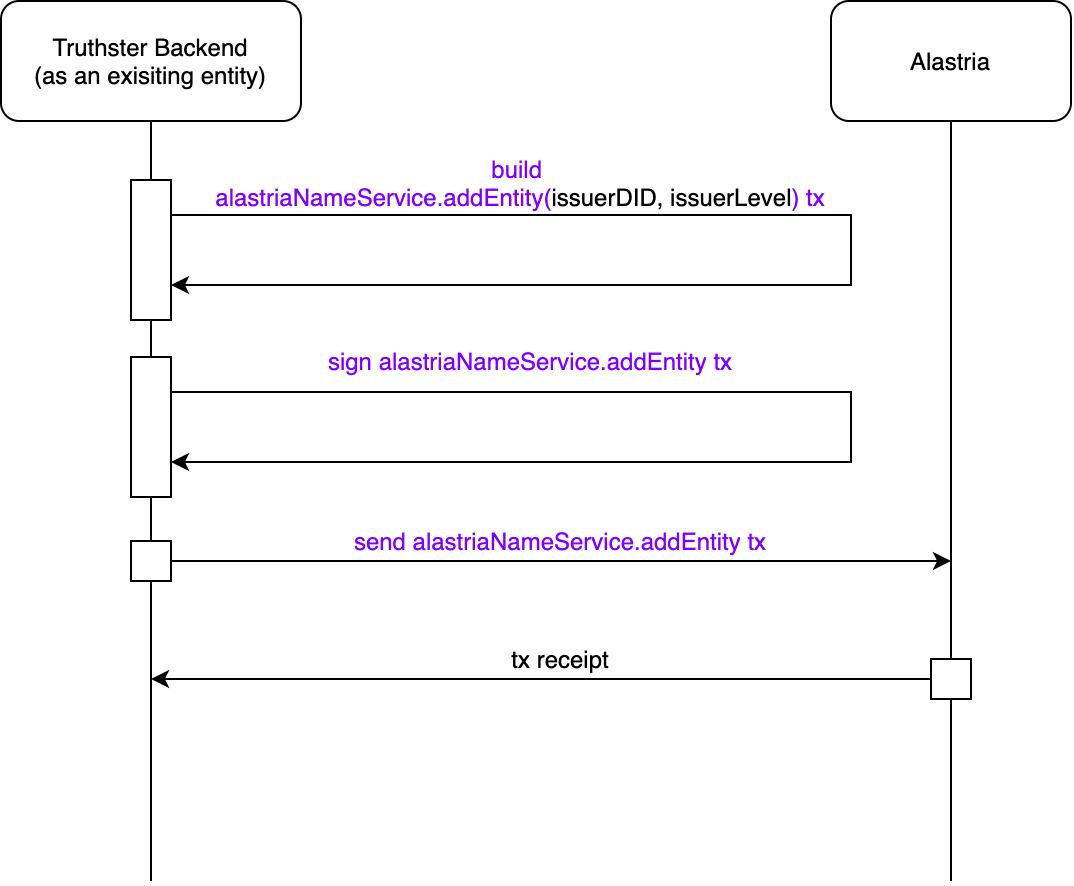
\includegraphics[width=0.8\textwidth]{images/addNewIssuer.png}
    \caption{Addition of a new issuer to the platform}
    \label{fig:addNewIssuer}
\end{figure}

\subsection{Delete exisiting issuer}

To delete a specific issuer with a low EIDAS level on the AlastriaID platform, the Truthster backend, which is an issuer with the authority to delete other issuers, must follow a series of steps. First, it creates a transaction called "identityManager.deleteIdentityIssuer," which takes the DID of the issuer to be deleted as a parameter. Next, the Truthster backend signs the transaction and sends it to Alastria. The transaction is executed, and the Truthster backend receives the transaction receipt as confirmation of the deletion. However, if the issuer with the given DID does not exist, the transaction is reverted with the related error. Overall, the deletion process is facilitated by the Truthster backend, which creates and signs the transaction to remove the specified issuer on the Alastria blockchain platform.
The process is represented in the Figure~\ref{fig:deleteIssuer}.

\begin{figure}
    \centering
    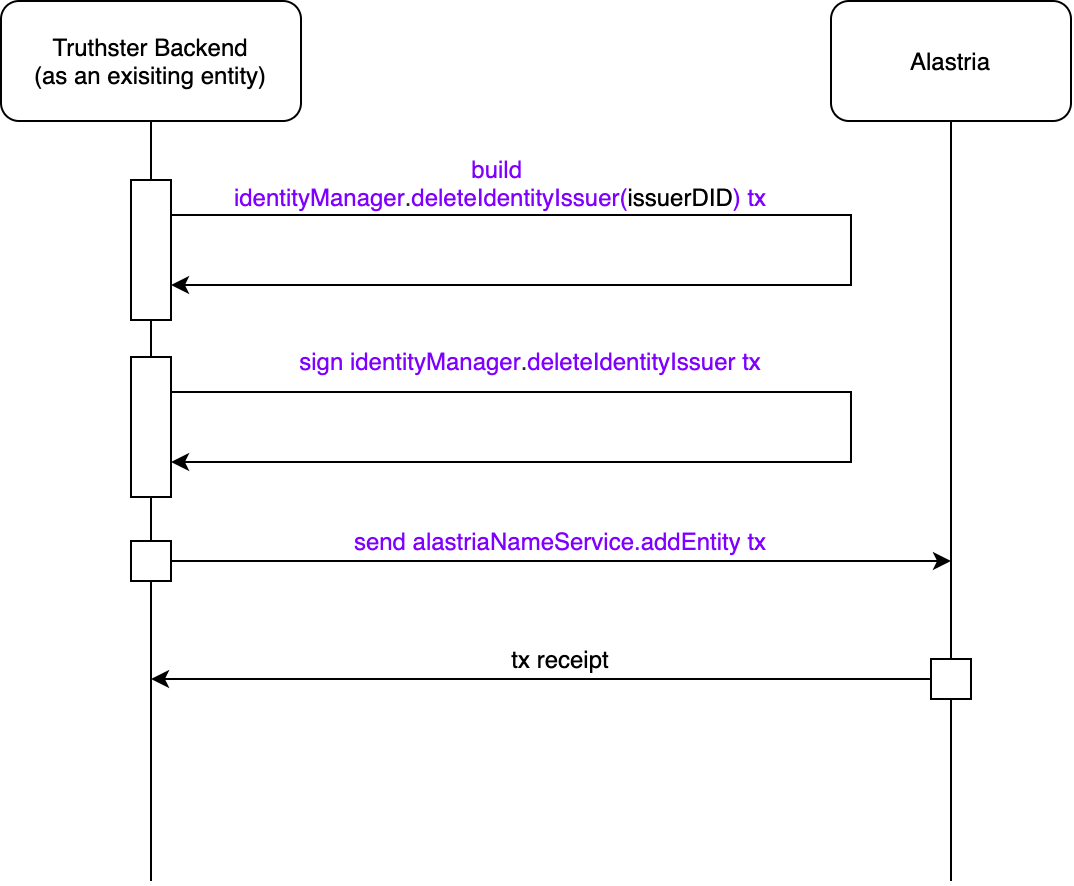
\includegraphics[width=0.8\textwidth]{images/deleteExistingIssuer.png}
    \caption{Deletion of an exisiting issuer from the platform}
    \label{fig:deleteIssuer}
\end{figure}

\subsection{Create new credentials}

Credentials are an important feature of the AlastriaID platform that allow users to access services provided by service providers. Credentials are essentially certifications issued by an authority on the AlastriaID platform that verify a user's identity or some other relevant piece of information. For example, a credential might confirm that a user is over the age of 18 or has completed a certain training program.\par
In this example (Figure~\ref{fig:updateSubjectPresentation}), to create new credentials, the subject (Bob) requests the issuer (Truthster back-end) to generate the required credentials. The issuer creates a token with the credentials and signs it using its private key. To allow the platform to verify the approval of the credentials, the signed token is hashed along with Bob's DID. The issuer sends the hashed credentials to Bob, who builds a transaction that includes the hashed credentials and the URI to the credentials as parameters. After signing the transaction with his private key, Bob sends the transaction bytecode to the Truthster back-end, which then sends the transaction to the Alastria blockchain. Once the transaction is confirmed, the Alastria blockchain sends the transaction receipt back to the Truthster back-end. By following these steps, the subject can obtain the required credentials from the issuer and add them to the Alastria blockchain for verification by service providers.

\begin{figure}
    \centering
    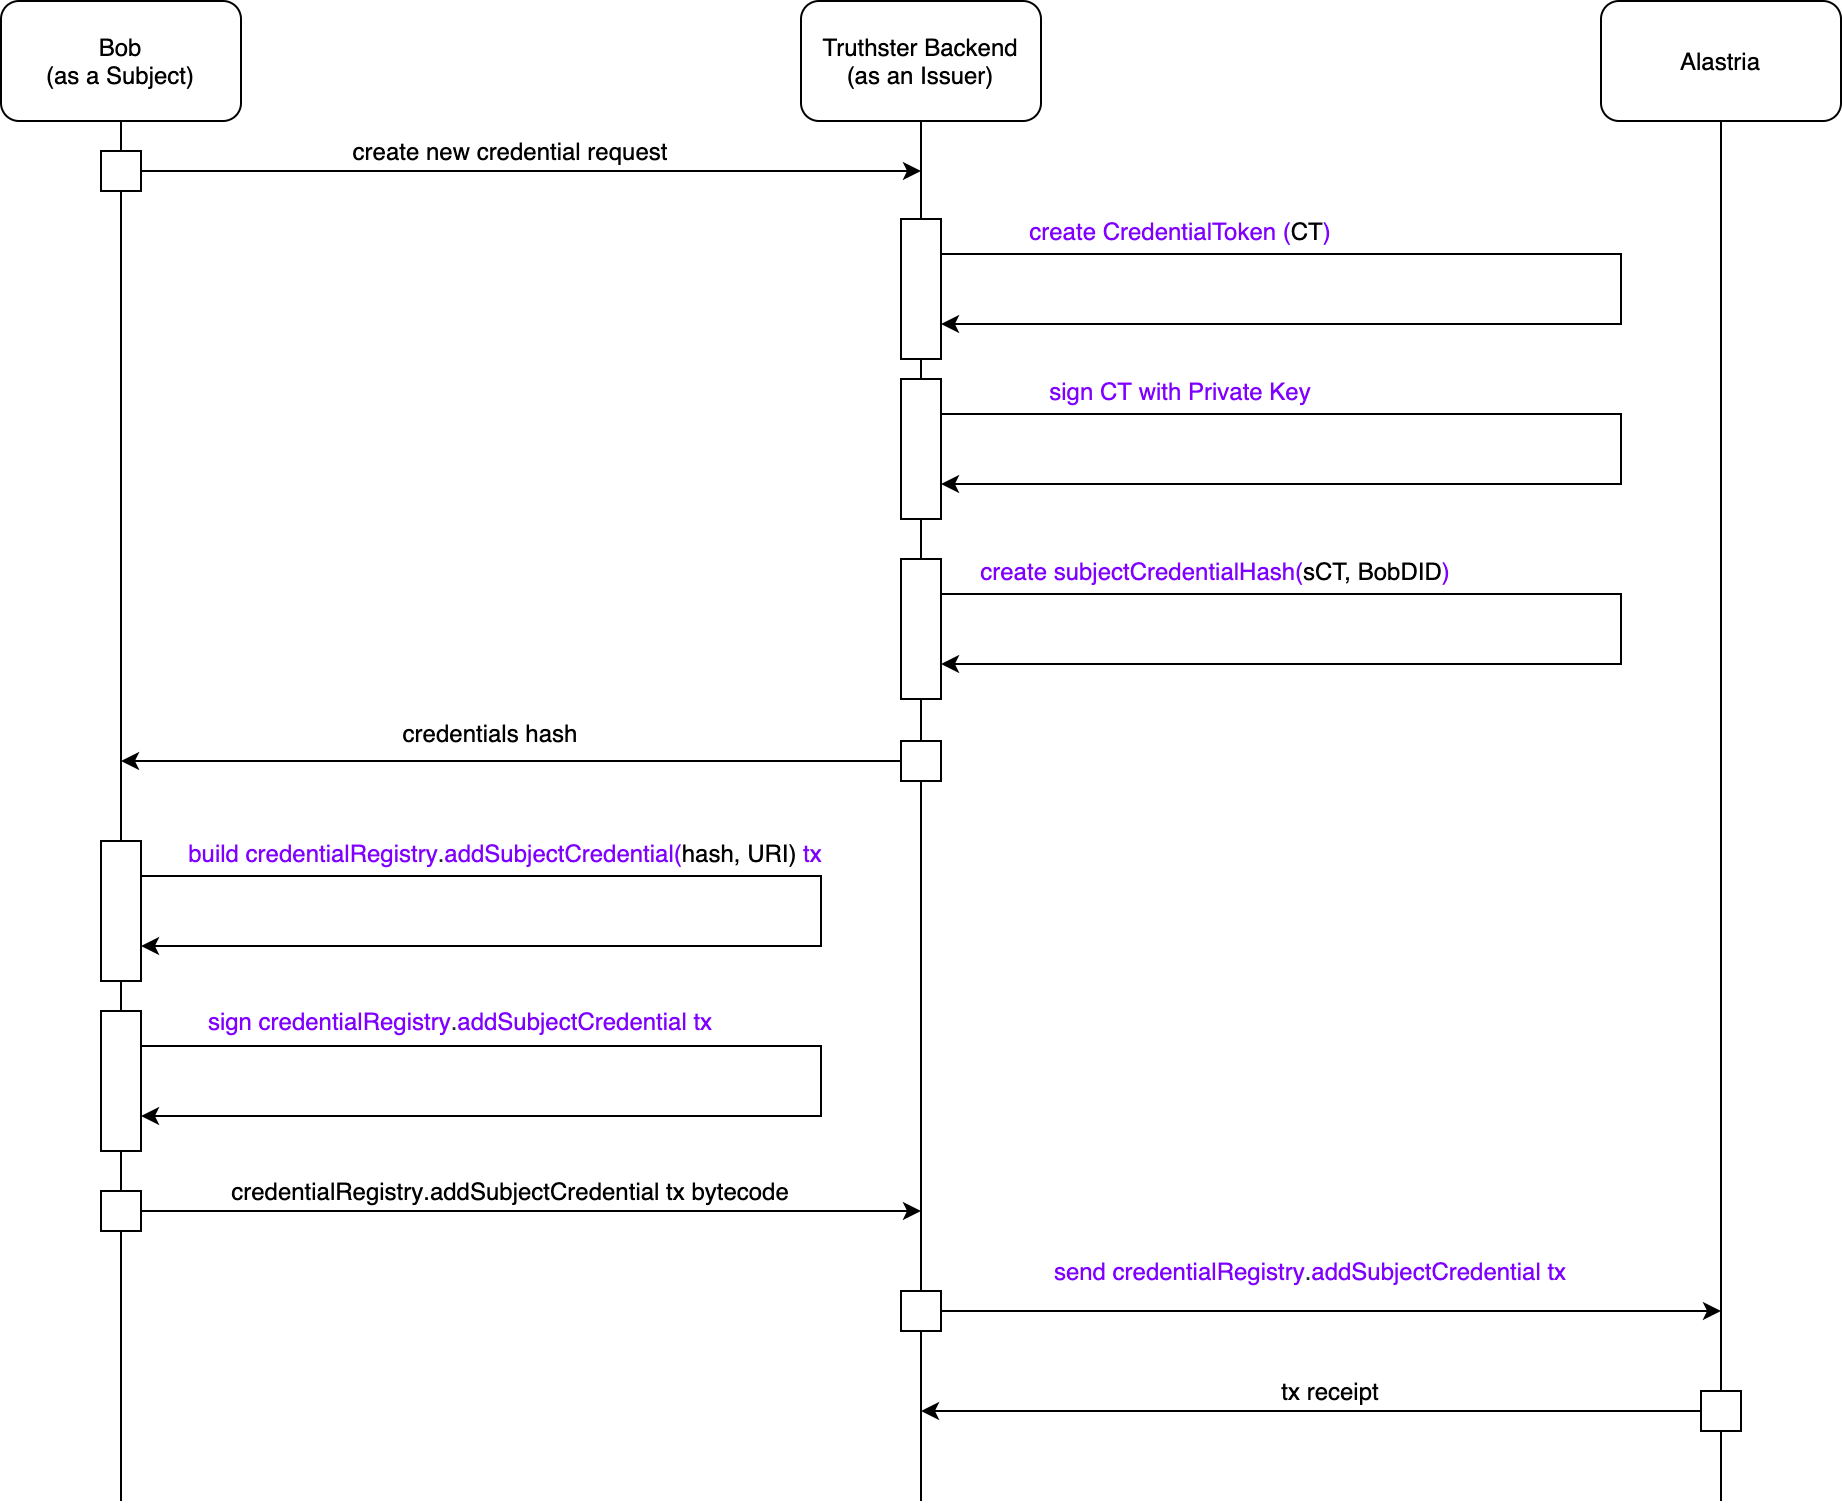
\includegraphics[width=0.8\textwidth]{images/createSubjectCredentials.png}
    \caption{Creation of new Subject credentials}
    \label{fig:createSubjectCredentials}
\end{figure}

\subsection{Create a new presentation}

A presentation is a collection of user credentials that are required by a service provider in order for a subject to access a specific service. The Alastria network provides a way to create, manage, and update these presentations using AlastriaID. In this guide, we will walk through the process of creating a presentation, updating it, and checking its status.

\begin{figure}
    \centering
    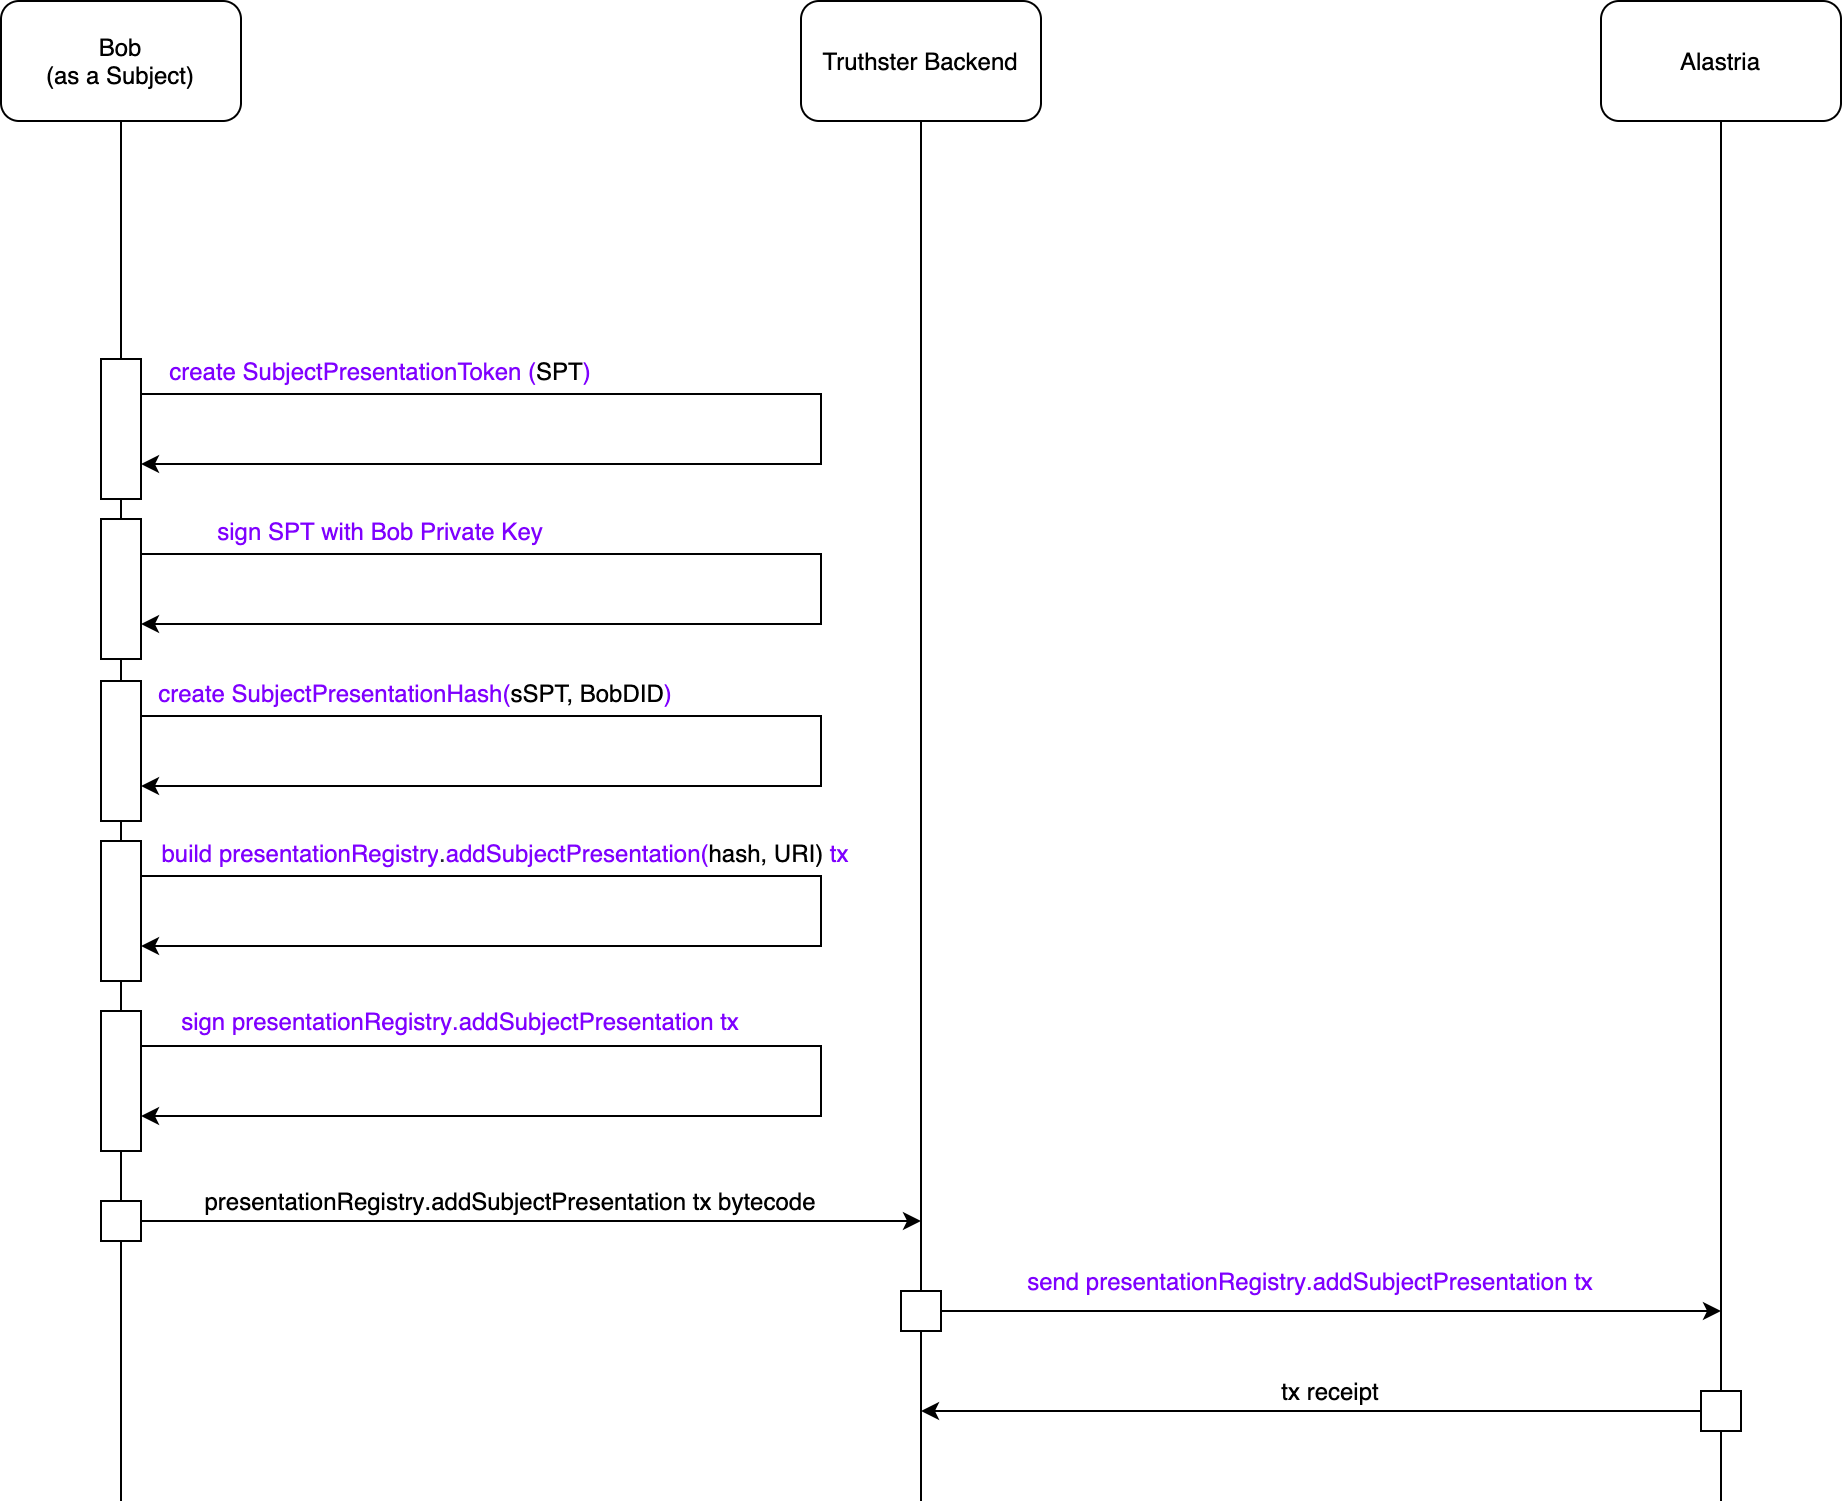
\includegraphics[width=0.8\textwidth]{images/createSubjectPresentation.png}
    \caption{Creation of a Subject presentation with AlastriaID}
    \label{fig:createSubjectPresentation}
\end{figure}

To create a presentation (Figure~\ref{fig:createSubjectPresentation}), the subject (Bob) needs to first authenticate themselves with their AlastriaID. The service provider (Truthster back-end) sends a presentation request to Bob, specifying the credentials that are required for the presentation. Bob then creates a SubjectPresentationToken (SPT) that contains the required credentials, and signs it using his private key. Next, he creates a presentation hash by combining the signed token (sSPT) with his DID. Bob then builds a transaction to add this presentation on Alastria, specifying the presentation hash and the URI of the presentation. After signing the transaction, Bob sends the bytecode to the Truthster back-end. The Truthster back-end then forwards the transaction to Alastria for execution and receives the transaction receipt back from Alastria.

\subsection{Update a presentation status}

To update an invalid or revoked presentation on the Alastria network (Figure~\ref{fig:updateSubjectPresentation}), the presentation owner (Bob) must build a transaction using the presentationRegistry.updateSubjectPresentation method. This transaction specifies the presentation to update and its new status as parameters. After signing the transaction, Bob sends it to the Truthster back-end. The Truthster back-end then forwards the transaction to Alastria, which executes the transaction. Once the transaction has been executed, Alastria sends the transaction receipt back to the Truthster back-end for confirmation. By following these steps, the owner of the presentation can ensure that service providers on the Alastria network only accept valid presentations.

\begin{figure}
    \centering
    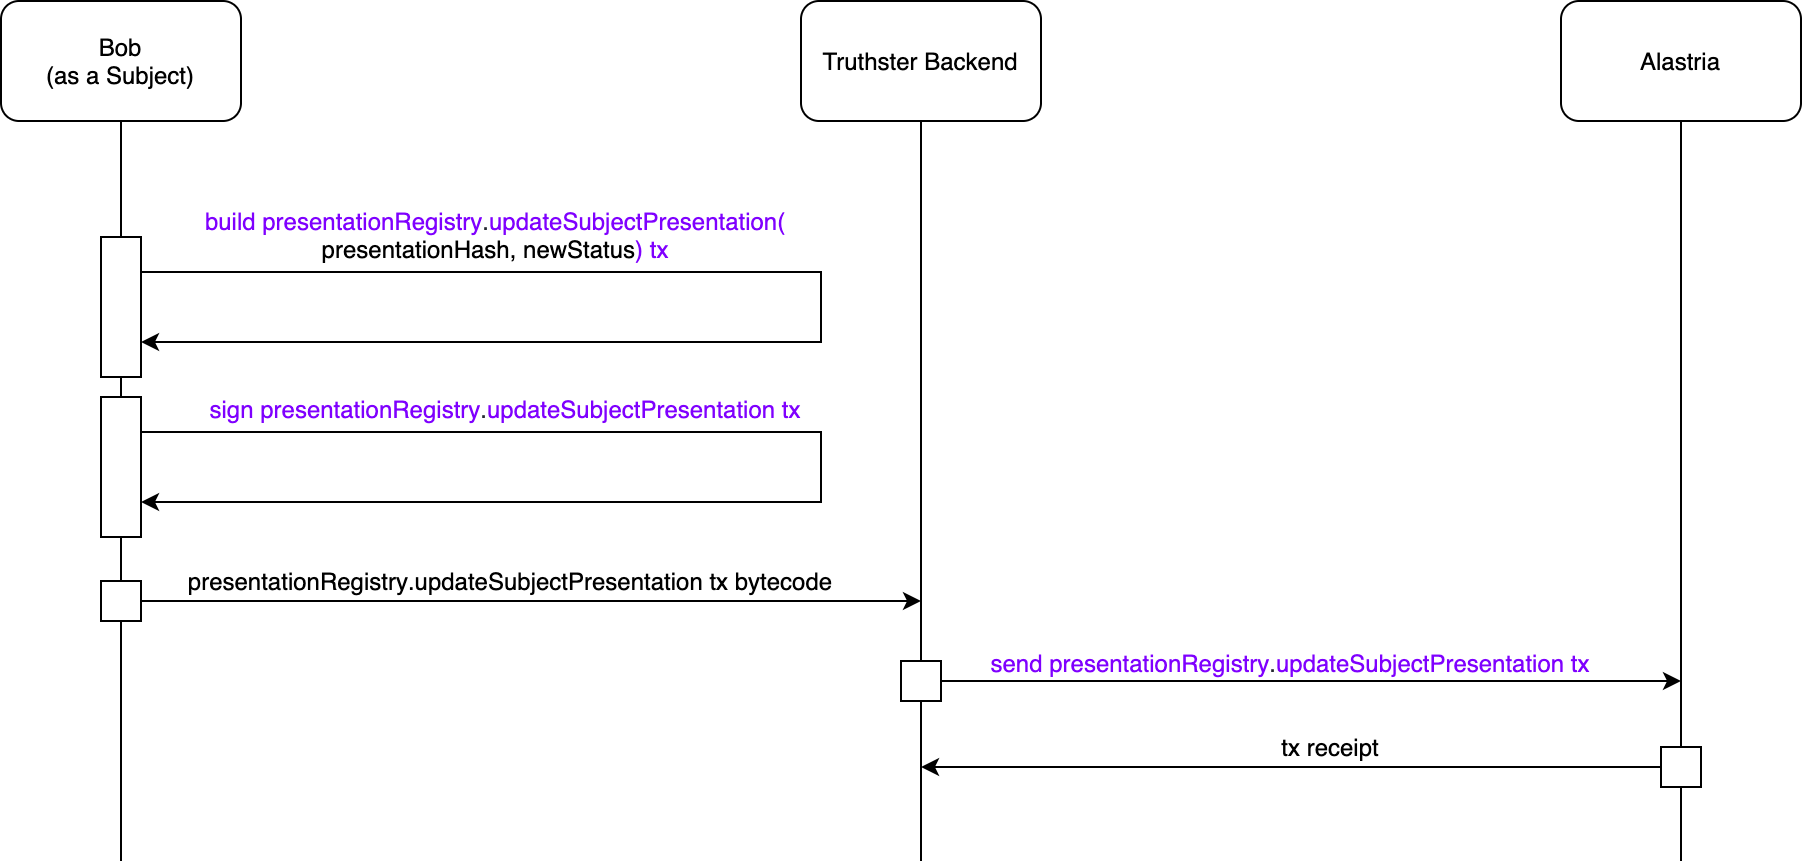
\includegraphics[width=0.8\textwidth]{images/updateSubjectPresentation.png}
    \caption{Update a Subject presentation status}
    \label{fig:updateSubjectPresentation}
\end{figure}

\subsection{Check a presentation status}

To check the status of a presentation on the Alastria network (Figure~\ref{fig:checkSubjectPresentationStatus}), a service provider can build a transaction using the presentationRegistry.getSubjectPresentationStatus method, including the subject presentation hash and subject DID as parameters. The Truthster back-end then sends this transaction to Alastria to execute, and upon completion, Alastria sends the transaction receipt back to the Truthster back-end for confirmation. By following these steps, a service provider can verify the status of a presentation and ensure that the subject attempting to access the service has valid credentials.
\textit{Notes}: in this process there is no need for signing a transaction since we are not writing on the Alastria blockchain, but just reading existing values.

\begin{figure}
    \centering
    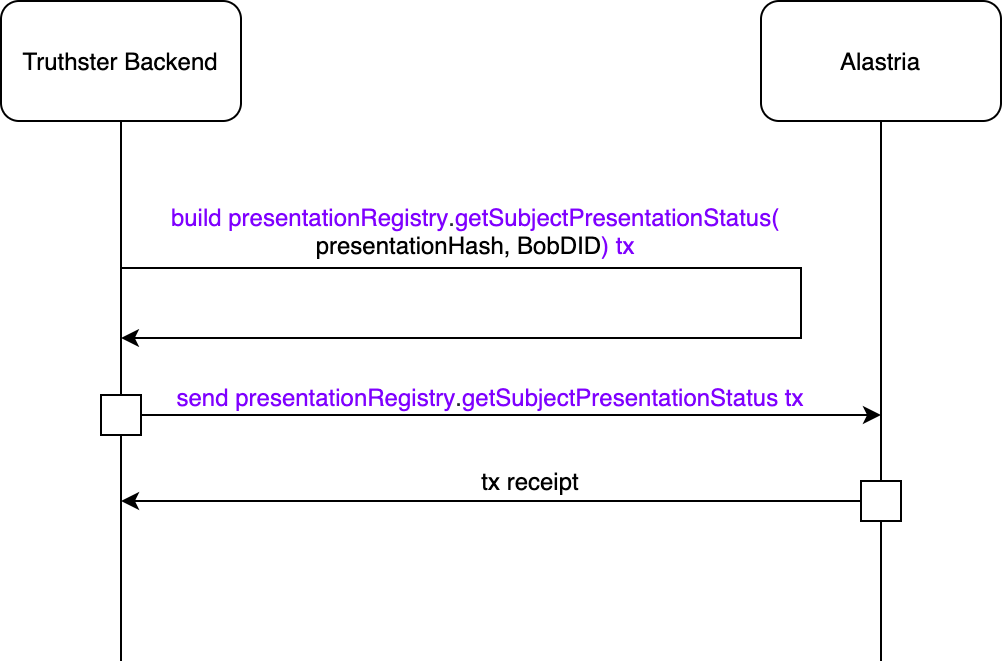
\includegraphics[width=0.8\textwidth]{images/checkSubjectPresentationStatus.png}
    \caption{Update a Subject presentation status}
    \label{fig:checkSubjectPresentationStatus}
\end{figure}

\subsection{AlastriaID - Summary}

After analyzing the most significant features offered by AlastriaID we can say that it is a powerful framework that provides a range of features for the management of identities and credentials on the Alastria blockchain network. With AlastriaID, users can create, manage, and revoke digital identities, as well as manage and share digital credentials. The framework enables the creation of decentralized applications that leverage the trust and security of the blockchain. Among the features provided by AlastriaID are the creation of a user's digital identity, the management of digital credentials issued by trusted authorities, and the presentation of those credentials to service providers in order to access their services. The framework also enables the revocation of credentials when needed and allows for the creation of presentations that can be checked for their validity. With some additional smart contracts and features, AlastriaID can be used as the backbone of a product, such as the Truthster system, that offers secure and reliable management of digital identities and credentials.




\chapter{Implementation}
\label{chapter:implementation}

As a collaborative project, Truthster involves various entities, including the University of Udine, the University of Perugia, a journalist, and a few IT companies. Due to its complex and long-term nature, the entire system has not yet been completed. However, we have prepared an initial prototype that provides a basic outline of the platform's functionalities and features. This prototype represents a starting point for us to structure and develop the platform further in collaboration with our partners. It will allow us to gather feedback, test different functionalities, and make necessary adjustments to enhance the platform's usability, reliability, and security. This prototype will also help us to communicate our vision effectively to potential stakeholders and investors, thereby paving the way for the further development and deployment of the system. Although the prototype is not the finished product, it serves as a solid foundation for the development of the final product, ensuring that the platform meets the needs of its users and stakeholders.\par
In this chapter, we will provide a detailed analysis of how the initial prototype of Truthster is implementing its basic functionalities. We will also discuss the missing components and how we plan to address them to meet both the functional and non-functional requirements of the system. Additionally, we will see the main scenarios of the Truthster system through a sequence diagram, discussing the implementation of the platform. We will also provide a component diagram to show how the system (final version) will be structured, along with a deployment diagram for the final version. These diagrams will provide a better understanding of how the various components of the platform interact with each other and how they are deployed on different nodes. This will help to provide a clearer picture of the overall architecture of the platform and how it can be scaled and maintained over time. Through this process, we aim to develop a comprehensive and reliable platform that can effectively address the needs of the journalism industry and provide a trustworthy and transparent source of information to the general public.

\section{Prototype structure}

Our prototype structure is designed to enable loosely coupled components, and we have accomplished this by using Docker \cite{docker} on a local virtual server located in the University of Udine. The system is composed of several containers, each representing a distinct service or function. The first container is an instance of a MongoDB database, where all the interview data and other related information is saved. In the second container, we have implemented our REST APIs, which are programmed to run on a Node.js server, as we have planned for the final solution. We have also created a third container that serves as a temporary interface, allowing us to interact with the APIs and MongoDB, and perform some basic operations. The Alastria node is already online, and it is provided by the Alastria Consortium, enabling us to take advantage of the blockchain technology in the prototype. This structure helps us to maintain modularity, scalability, and flexibility, and makes it easier for us to add, remove or modify components in the future as the project evolves. In Figure~\ref{fig:prototypeSchema} you can see how the prototype is structured.

\begin{figure}
    \centering
    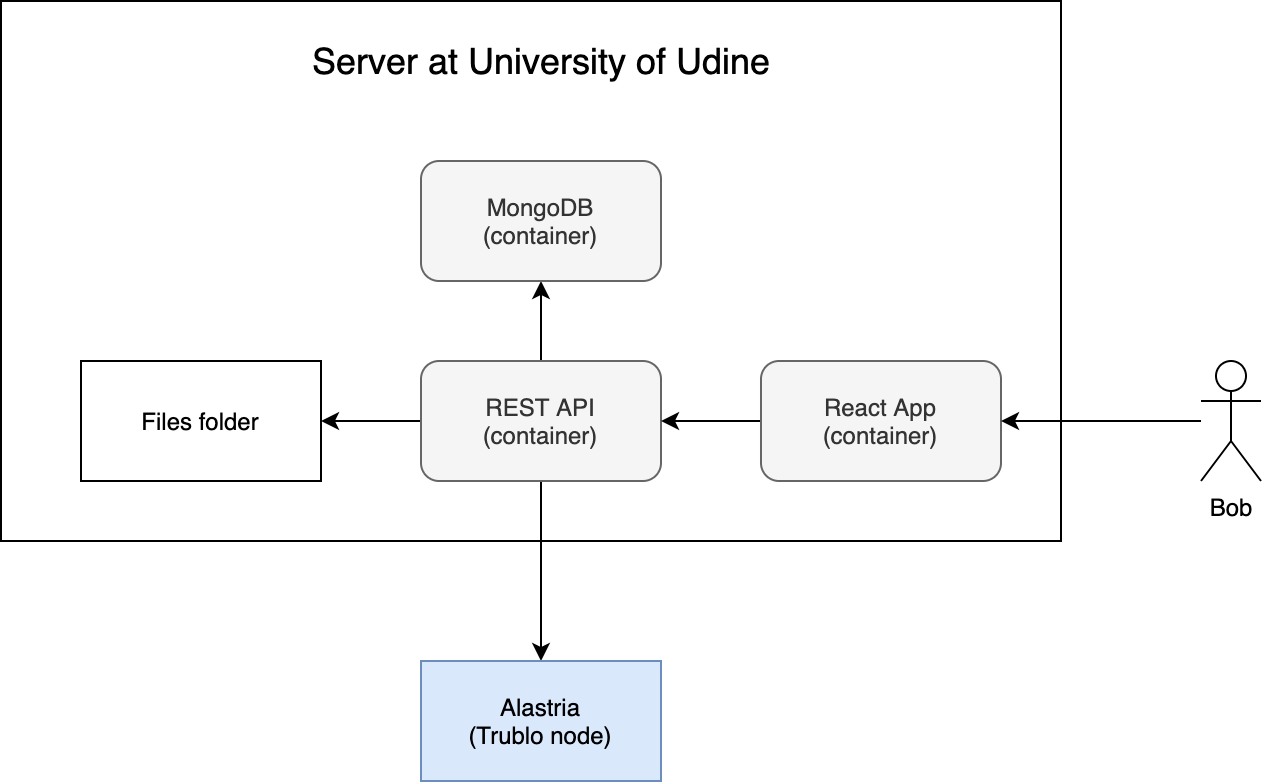
\includegraphics[width=0.8\textwidth]{images/prototypeSchema.png}
    \caption{Design of the Truthster system prototype}
    \label{fig:prototypeSchema}
\end{figure}

\section{Prototype explanation}

In this section, we will provide an in-depth analysis of how our prototype for Truthster works.\par
In our prototype, as previously mentioned, we have three containers that reside on our server, along with a "Files folder" located outside the containers. This folder is encrypted and contains the interview files that are also encrypted since they are large and may be lost in case of a container reset. This is because containers have temporary memory that lasts only for their entire life. By storing the interview files in an encrypted folder outside the containers, we can ensure that the files are not lost and are easily accessible by the back-end and other system services.\par
The React app container serves as the interface for users like Bob, who want to access the functions of the Truthster platform. Bob, a journalist, accesses the web app on his PC or mobile device, creates a new project related to the interview he wishes to conduct, and enters all the necessary interview information, such as GPS position, interviewee name, project name, location, and consent agreement. The project creation can be done before the interview as it is not a locked element. After confirming the project, it is sent as a JSON to the back-end container, which stores the data on the MongoDB instance using REST APIs.\par
After Bob has finished the interview, he can load the related media onto the web app from his PC or mobile device. The media is then passed to the back-end container, where it is encrypted and stored in the "Files folder" on the server. A link to the file is also stored in the interview project on the MongoDB instance, allowing Bob to easily access the file in the future. This ensures that the interview media is securely stored and easily accessible for future use.\par
In this initial prototype, the Alastria blockchain is not yet directly integrated into the system, but it has been used in a separate manner. At the moment, Bob is not required to log in using AlastriaID, as we are still working on the API and mechanics to implement it in the most secure and effective way possible.

\section{Blockchain implementation}

Alastria is a unique permissioned blockchain platform, as it requires a whitelisted IP address to access its network. In order to gain access to the production version of Alastria, the RedB network, our server went through a simple process to be whitelisted. This allows Truthster to interact with Alastria through the REST API container, which ensures safe and controlled access to the blockchain.
One of the key features of Alastria is that it is an EVM blockchain, which means its runtime is based on an Ethereum Virtual Machine \cite{evm}. This feature allows calls and transactions to be made on Alastria in the same way as other public chains such as Ethereum \cite{ethereum}, Polygon \cite{polygon}, or Moonbeam \cite{moonbeam}. While there are many public blockchain platforms available, Alastria stands out for its permissioned nature and its close association with the Spanish public and private sectors.\par
Having this in mind we have leveraged the power of existing libraries such as Ethers \cite{ethers} and Web3 \cite{web3}, which enable us to access blockchain data, read and send transactions that are compatible with Node.js. With this capability, we have configured the REST API server in such a way that it is easy to add REST calls that interact with the blockchain, and all of the calls can be easily filtered through the back-end for better security. By taking this approach, we can ensure that all blockchain interactions are carried out in a safe and secure manner, without any direct exposure to external factors that may compromise the integrity of the system.

\subsection{Truffle and Ganache}

In order to effectively connect to the Alastria RedB network and build a complete prototype for the Truthster platform, we first had to familiarize ourselves with the Ethereum Virtual Machine (EVM) model. To do this, we utilized a local blockchain called Ganache and the Truffle framework. Through this process of studying and testing the EVM model, we were able to gain a deeper understanding of how the blockchain works and how we can interact with it using our application. This knowledge allowed us to develop and test our smart contracts and other blockchain-related functionality in a safe and controlled environment before deploying it to the production network.\par
The Truffle framework provided us with a comprehensive set of tools and utilities for developing, testing, and deploying smart contracts, making our development process more efficient and streamlined. These tools include built-in smart contract compilation, linking, deployment, and binary management, making it easier for developers to manage their code. Additionally, Truffle offers advanced debugging features, such as breakpoints, variable analysis, and step functionality, to ensure the accuracy and reliability of the smart contract. The framework also provides a deployment and transaction interface with MetaMask to protect developers' mnemonic and an interactive console for direct contract communication.\par
To facilitate rapid development, Truffle also offers automated contract testing and a scriptable, extensible deployment and migration framework. The tool also offers network management capabilities, allowing developers to deploy their smart contracts on any number of public and private networks. Finally, Truffle includes package management with NPM, using the ERC190 standard, and a configurable build pipeline with support for tight integration. With its comprehensive set of features, Truffle is a world-class development framework for Ethereum smart contracts that enhances developer productivity and efficiency.\par
We used the contract of the AlastriaID library and deployed our version on Ganache to test its functionalities. However, to achieve a better and more complete prototype, these contracts have to be used along with JWT tokens and the other features offered by the Alastria identity library. This is necessary in order to get a product that resembles the final Truthster platform in terms of its most important functionalities. By utilizing the Truffle framework and Alastria identity library, we aim to build a fully-functional and secure platform that can effectively combat fake news and promote truth and transparency in journalism.

\section{Prototype status}

The prototype that we have implemented has a limited set of functionalities. As previously mentioned, the Truthster project is a collaborative effort that involves multiple entities, and thus this prototype represents only the initial stage of the platform's development. Moving forward, we will use this prototype as a starting point to test and build upon the other functionalities required for the final product.
The current version of the prototype serves as a proof of concept for the basic features of Truthster, such as creating new projects, managing interview data, and interacting with the Alastria blockchain. However, there are many more features and capabilities that must be added to the platform to achieve its full potential.\par
For example, one major aspect of the project that we are currently working on is the integration of the Alastria identity library, which will allow for more secure and authenticated interactions with the blockchain. Additionally, we plan to develop more advanced functionality for managing interview data, such as adding tags and categories to make it easier to search and analyze large volumes of data.\par
Overall, the current prototype represents a first step in the development of Truthster, and we look forward to working with our partners to build a comprehensive and robust platform that meets the needs of journalists, researchers, and other users in the field of digital media.

\section{Truthster main scenarios}

In this section, we will provide a sequence diagram that represents the implementation of the most significant scenarios of the Truthster platform. This diagram serves as a plan for our development process and will provide a clearer picture of how the platform will be structured and how its various components will interact with each other.\par
The diagram includes the following scenarios that are represented in the Figure~\ref{fig:sequenceDiagram}.

\begin{enumerate}

    \item Media getting
    \item Create new project
    \item Save interview data and metadata
    \item Send authorization link
    \item Request interviews information

\end{enumerate}

\begin{figure}
    \centering
    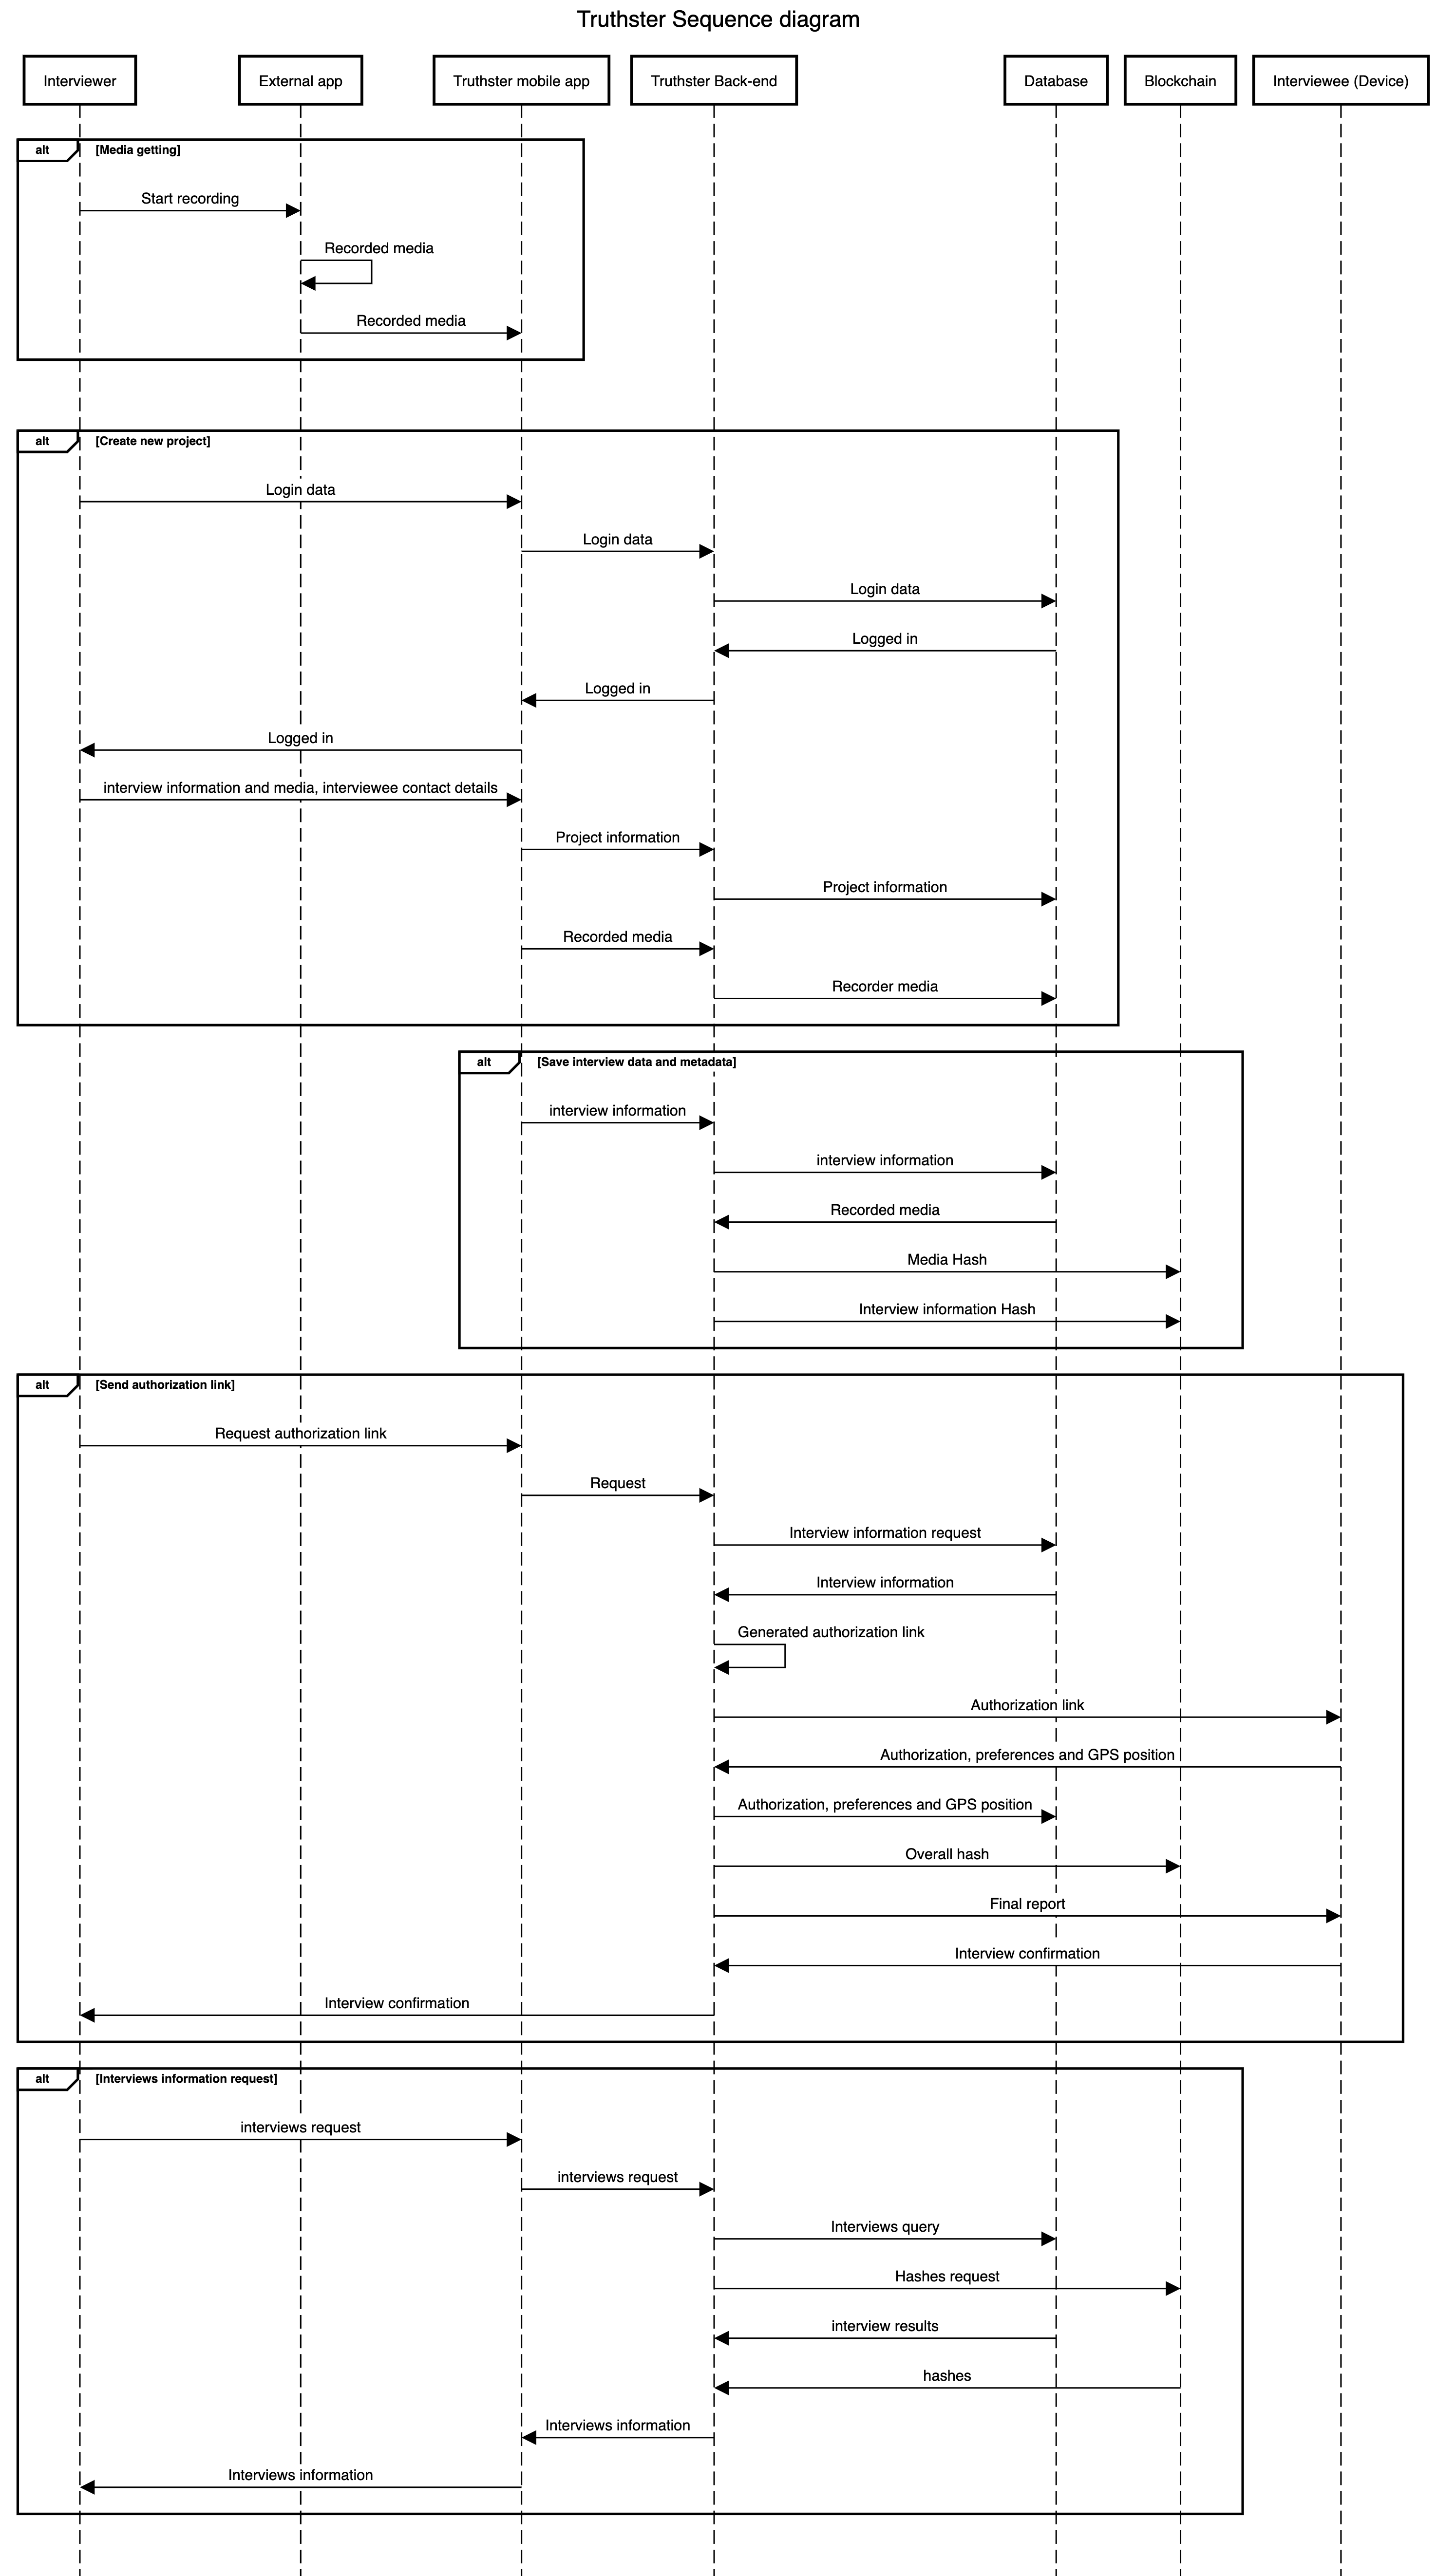
\includegraphics[width=0.8\textwidth]{images/sequenceDiagram.png}
    \caption{Sequence diagram of the Truthster main scenarios}
    \label{fig:sequenceDiagram}
\end{figure}

\subsection{Media getting}
\label{mediaGetting}

In this scenario, a journalist uses a third-party app to record an interview, and then uploads the media to the Truthster platform through the mobile app. After the media is uploaded, it is encrypted and sent to the back-end for storage in a secure database. The specific details of this process are not yet defined, but will be established in the further development of the platform. The primary objective of this scenario is to demonstrate how the platform will enable journalists to securely and easily upload media files to the Truthster system for safe and transparent storage.

\subsection{Create new project}
\label{createNewProject}

In this scenario, the journalist initiates the process by logging into the platform through the mobile app. The app then sends the login information to the back-end for verification. Once the credentials are authenticated, the back-end sends the login response back to the user, allowing them to proceed. After successful login, the journalist inputs all the necessary information to create a new project, including interview information, interview media, and interviewee contact details. This information, along with the recorded media from the \nameref{mediaGetting} scenario, is sent to the back-end, where a new project is created and stored in the platform's database.

\subsection{Save interview data and metadata}
\label{saveDataAndMetadata}

In this scenario, the interview information obtained in the \nameref{createNewProject} scenario is processed by the back-end. Some of this information is sent to the database, the metadata that has not been previously passed. The recorded media is fetched from the database and then the hash of the media and the interview information is registered on the Alastria blockchain using a custom transaction. This process ensures the immutability and integrity of the interview data, providing a tamper-proof solution that can be verified when needed from both journalists and interviewees.

\subsection{Send authorization link}
\label{generateAndSendLink}

In this scenario, the interviewer requests the system to generate an authorization link that will be sent to the interviewee to obtain their consent. The system fetches all the necessary information from the database, generates the link, and sends it to the interviewee. The interviewee can then review the interview and add any necessary information. Once the interviewee has completed the review and provided their consent, the system is notified and the interviewer is then able to proceed with publishing the interview content. An overall hash of the information and the interviewee's consent is stored on the Alastria blockchain. This process ensures that all parties involved have provided their consent and that the information is accurate before it is published on the platform.

\subsection{Request interviews information}
\label{requestInterviewsInformation}

In this scenario, the interviewer requests information about previous interviews through the mobile app. The request is sent to the back-end, which processes the request by retrieving the relevant information from both the blockchain and the database. Finally, the back-end provides the requested information to the interviewer through the mobile app. This allows the interviewer to easily access and review past interviews stored on the platform. The use of both the blockchain and the database ensures the security and accuracy of the stored information.

\section{Component diagram}

The component diagram in Figure~\ref{fig:componentDiagram} illustrates which are the different components of the Truthster platform. The main components include the user interface, which consists of a mobile application and a website, the back-end server, a database management system (DBMS), and a blockchain.\par

The user interface is responsible for handling user authentication and querying the server, which in turn checks the user credentials in the DBMS. The UI is also responsible for project creation, which involves collecting and sending all necessary data to the back-end server for storage in the DBMS. Finally, the user interface manages permissions and sends a request to the server to write the media hashes in the blockchain. This process ensures the immutability and transparency of the stored data.\par
The back-end server is responsible for handling communication between the user interface, the DBMS, and the blockchain. It processes user requests, retrieves and stores data from the DBMS, and sends data to the blockchain for secure storage and verification.\par
The DBMS stores all information related to the interviews, including interviewee contact details, metadata, and media content. In the later stages of the project, an additional SQL database will be added to store data about interviewers and interviewees.\par
The blockchain is represented as an Alastria node that provides access to the blockchain infrastructure. It stores the hashes of the media and interview information, providing a secure and tamper-proof solution for storing and verifying interview data.

\begin{figure}
    \centering
    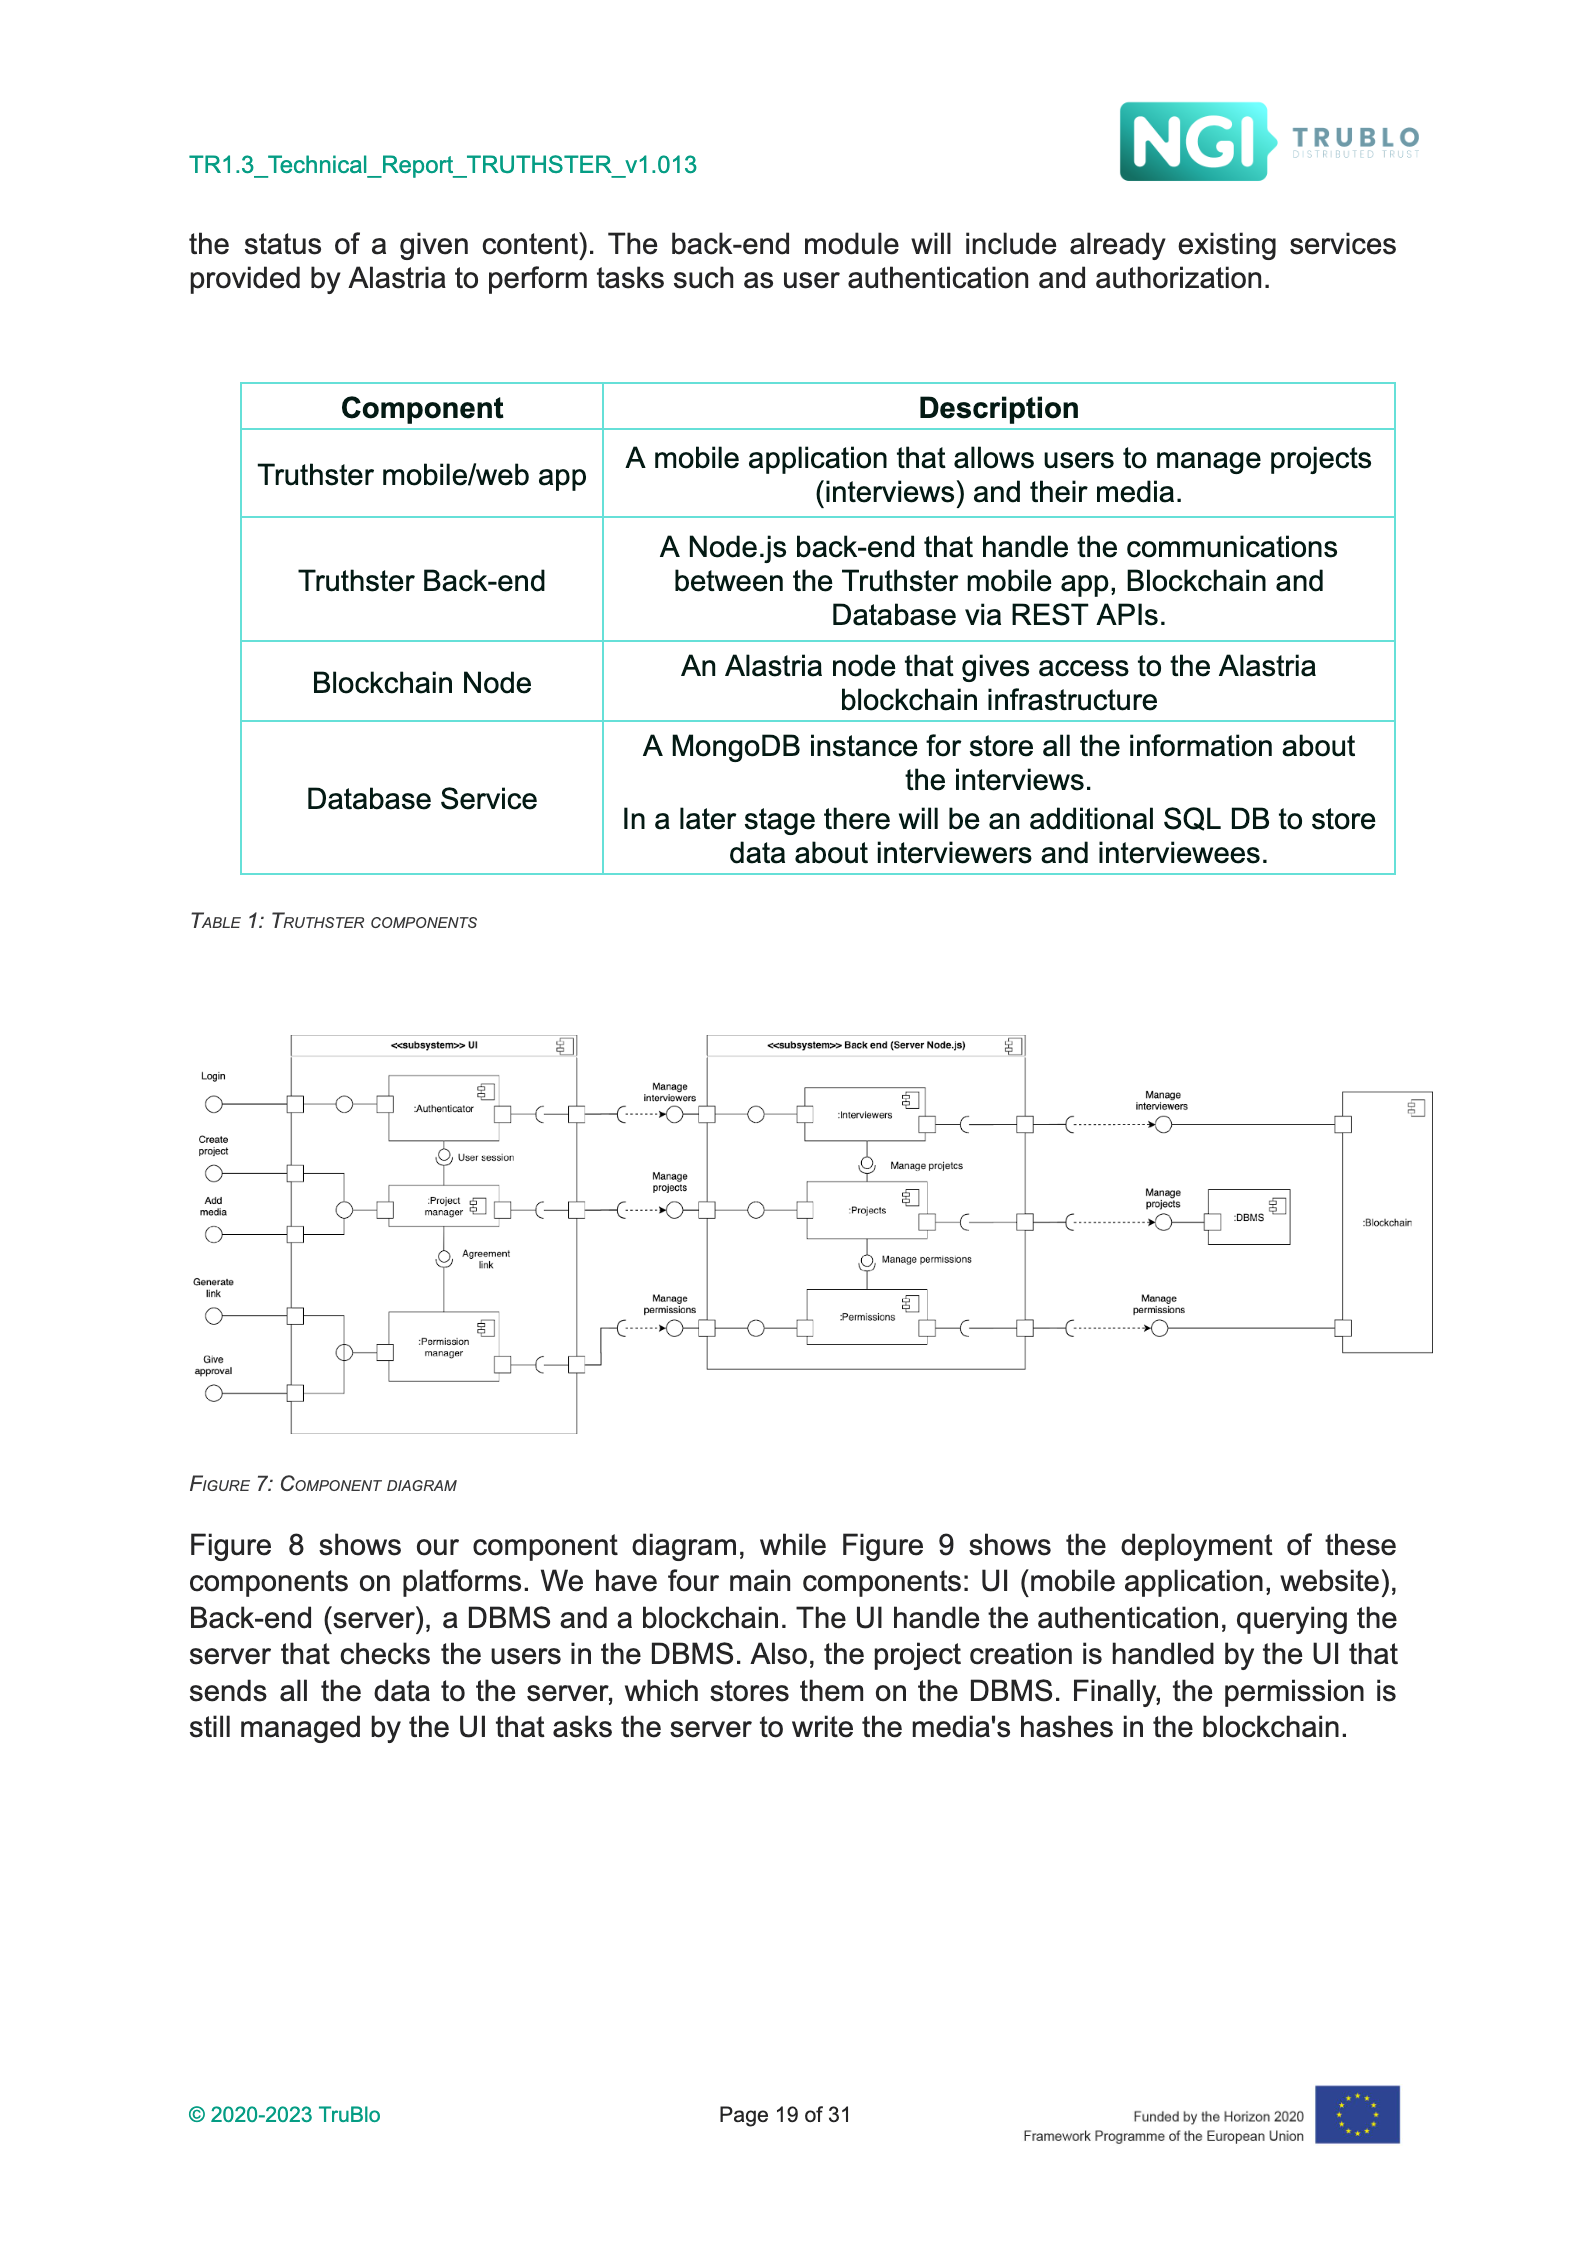
\includegraphics[width=0.8\textwidth]{images/componentDiagram.png}
    \caption{Truthster components diagram}
    \label{fig:componentDiagram}
\end{figure}

\section{Deployment diagram}

A deployment diagram is a type of UML diagram that depicts the physical components of a software system and their relationships. It shows how the software system is deployed on hardware, as well as how the hardware components interact with each other.

The Truthster deployment diagram, in Figure~\ref{fig:deploymentDiagram}, illustrates the deployment of the different components of the Truthster platform.\par
It consists of four components: 

    \begin{itemize}

        \item An Android app (represents the user interface)
        \item A Back-end container
        \item A DBMS container
        \item A blockchain container

    \end{itemize} 

The Android app resides on a device and serves as the user interface for accessing the Truthster platform. The back-end container, built with Docker, handles the communication between the user interface, the DBMS container, and the blockchain container. The DBMS container stores all the information related to the interviews, while the blockchain container represents the Alastria node that the back-end connects to in order to send transactions and retrieve stored data. Together, these components create a scalable and reliable platform that can effectively address the needs of the journalism industry and provide a trustworthy and transparent source of information to the general public.

\begin{figure}
    \centering
    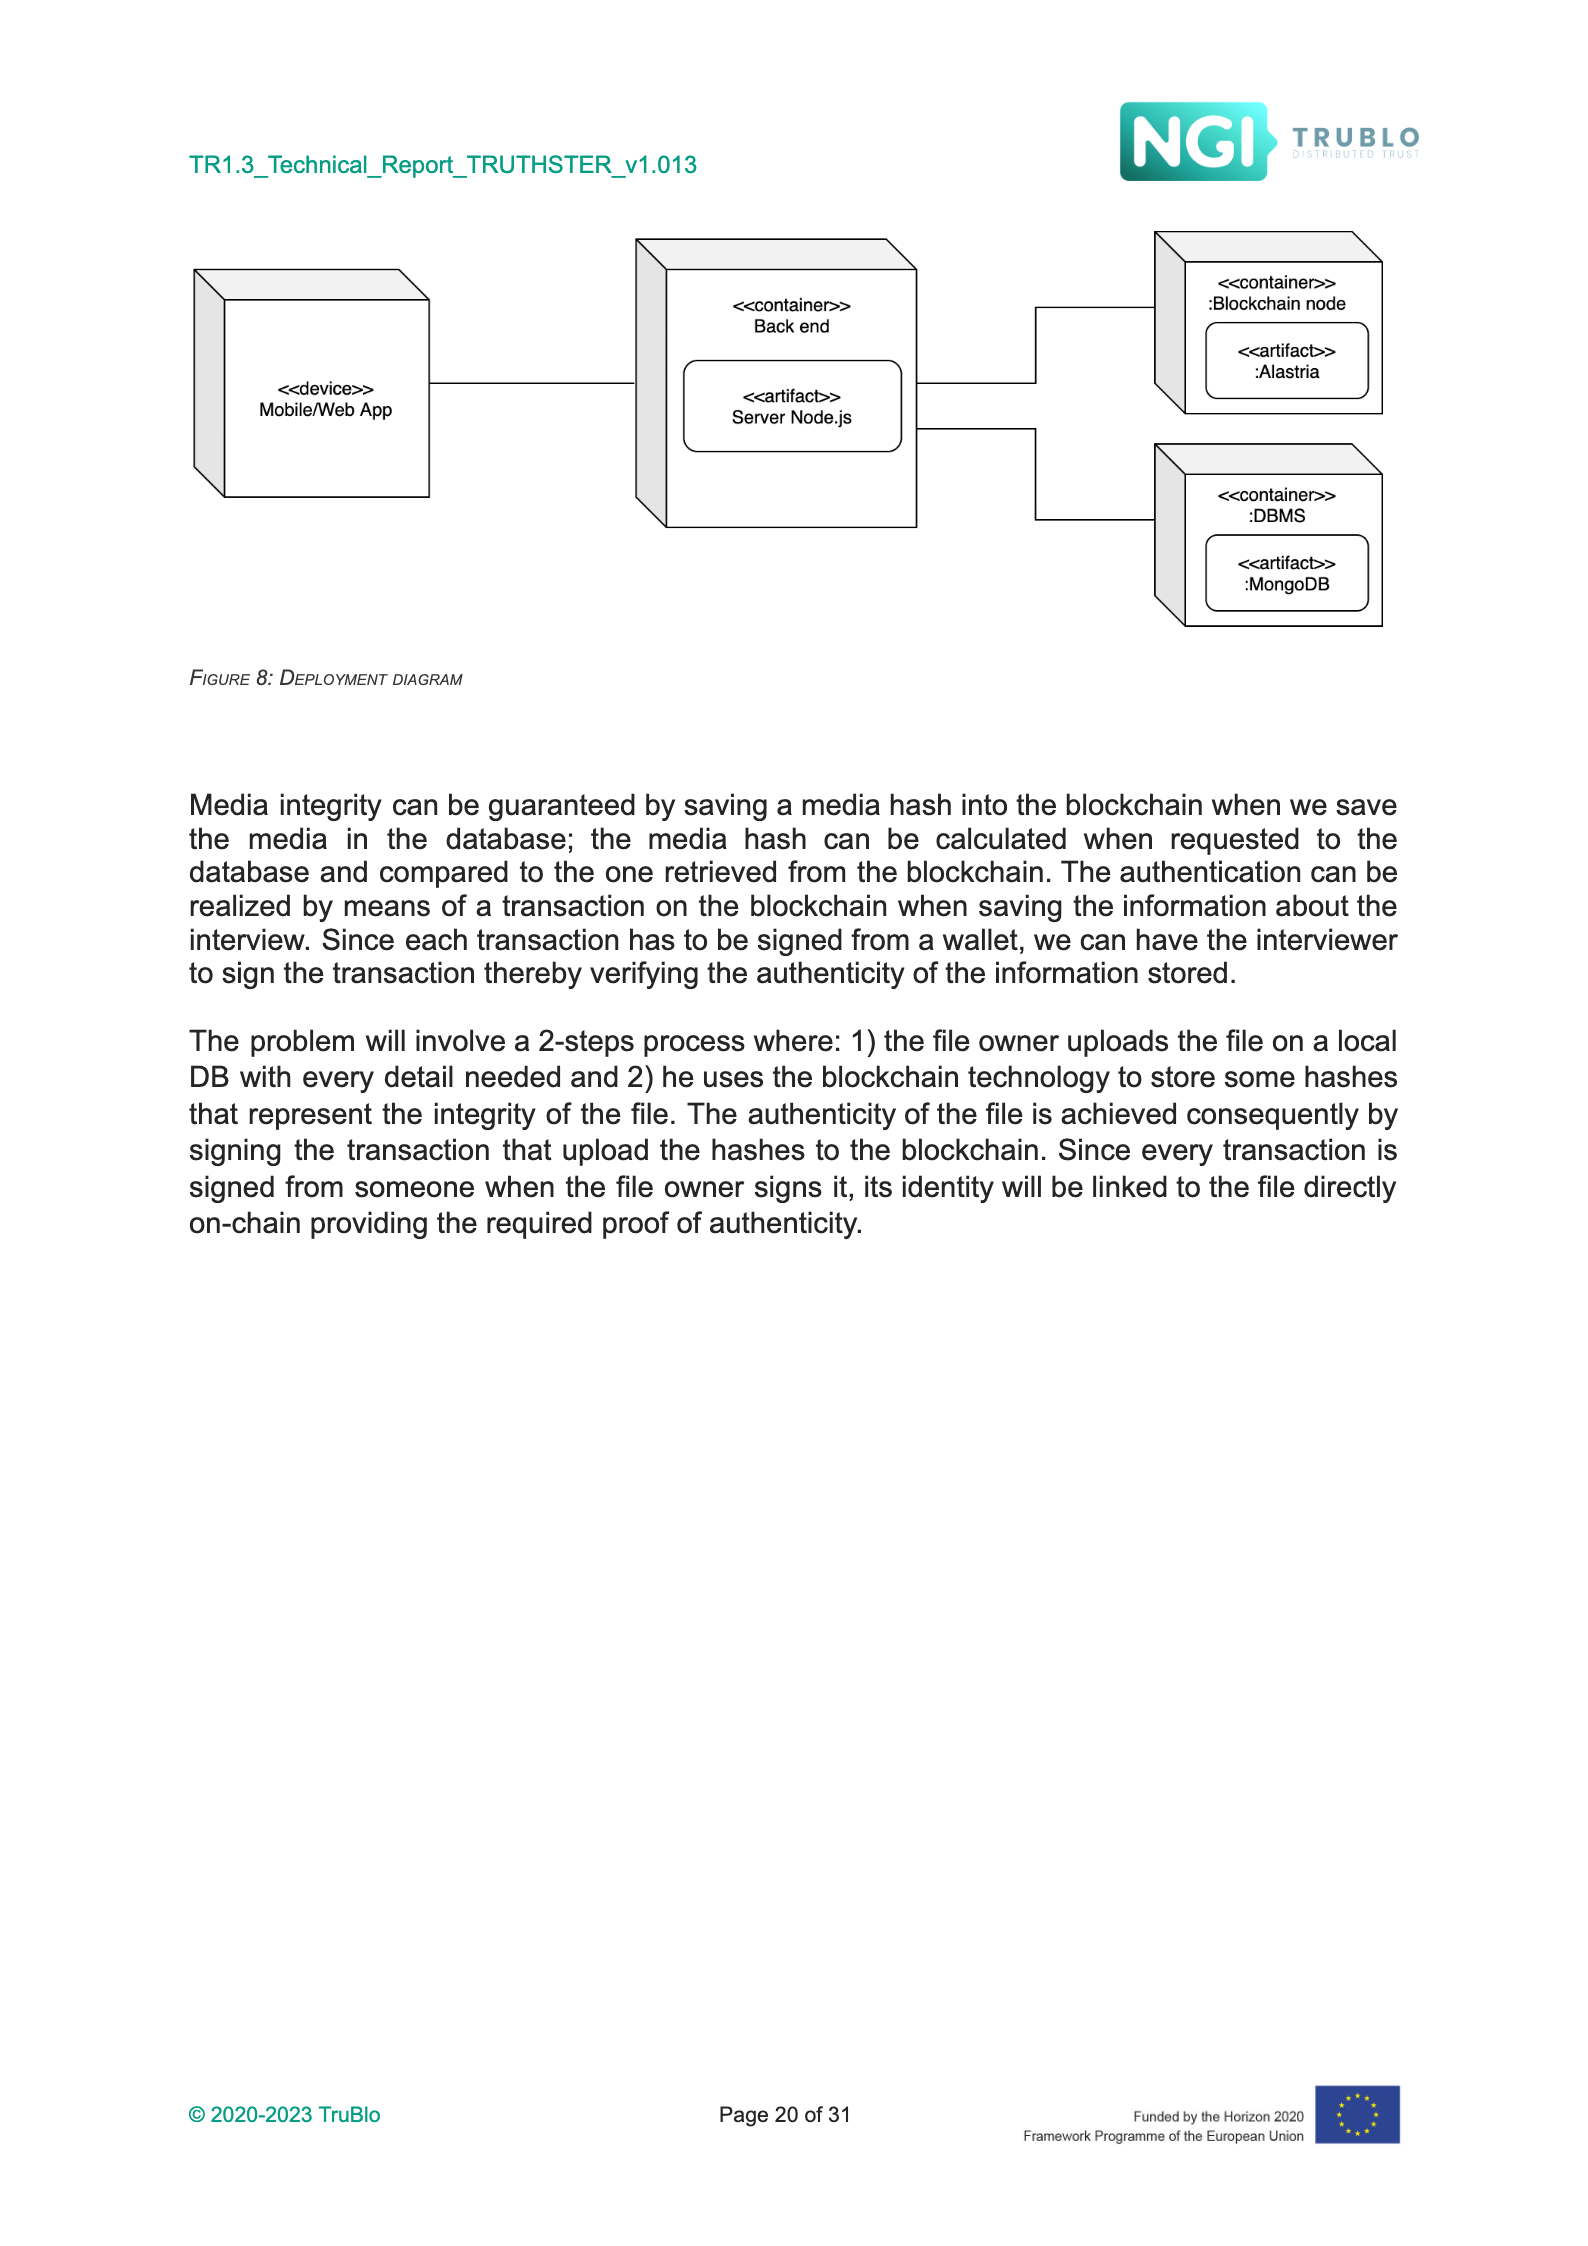
\includegraphics[width=0.8\textwidth]{images/deploymentDiagram.png}
    \caption{Truthster deployment diagram}
    \label{fig:deploymentDiagram}
\end{figure}

\chapter{Testing and validation}
\label{chapter:testingAndValidation}

In this chapter, we will go through the process of testing and validation for the Truthster platform. As we have previously discussed in the \nameref{problemAnalysis} chapter, there are a set of functional and non-functional requirements that the platform must meet in order to provide an effective solution for the journalism industry. In this chapter, we will detail how we have tested the initial prototype and how we plan to further test and validate the platform in order to ensure that all requirements are met by the final product.\par
We will begin by discussing the requirements that the prototype has already satisfied and those that still need to be addressed in the final version. We will then detail how we plan to meet these requirements through rigorous testing and validation processes, including unit testing, integration testing, and system testing. Through these processes, we aim to identify any potential issues or bugs in the platform and address them in a timely and effective manner.\par
Ultimately, our goal is to provide a comprehensive and reliable platform that meets the needs of the journalism industry and provides a trustworthy and transparent source of information to the general public. Through thorough testing and validation, we aim to ensure that the final Truthster platform meets these goals and provides a secure and efficient solution for managing and sharing interview data in compliance with GDPR.

\section{Prototype analysis}

The actual prototype of the Truthster platform, despite being incomplete, already satisfies some functional and non-functional requirements. A functional requirement is a specific task or feature that a system or software must perform, while a non-functional requirement is a characteristic that the system or software must possess to ensure optimal performance, reliability, and security. In this section, we will discuss the functional and non-functional requirements that the current Truthster prototype fulfills.\par
\subsection{Functional requirements}

    \begin{enumerate}

        \item \textbf{Embed authorship and legal details}: the Truthster prototype partially fulfills this requirement by enabling the storage of all necessary information and documentation related to a specific interview in the database. This ensures that authorship and legal aspects can be properly recorded and cannot be manipulated. However, the consent handling is not yet implemented in the prototype, although the system's structure enables a quick implementation of this feature.
        \item \textbf{Secure and manage interview data}: the Truthster prototype satisfies this requirement by implementing several features to ensure the confidentiality and security of interview-related data. Firstly, the prototype stores all interview media files in an encrypted format, preventing unauthorized access to the media content. Secondly, the data is stored on a server that is only accessible to authorized users, ensuring that only authenticated users can access the information. This provides an additional layer of security for the data, protecting it from potential data breaches. Furthermore, the prototype allows for the organization of data in a way that associates it with a specific project. This feature facilitates the retrieval and management of data, ensuring that interview data is easily accessible and searchable by authorized users. The data includes not only the media content, such as video interviews, but also any relevant legal documents, user terms, and agreement conditions, ensuring that all the required information is accessible in one place.
        \item \textbf{Certify and verify digital media with blockchain (Alastria)}: this requirement is partially satisfied by the prototype as it already integrates with the Alastria blockchain. However, the prototype lacks the capability to verify the digital media with blockchain by checking the hash of the encrypted version stored on the database server. To fully satisfy this requirement, a smart contract can be created that stores the media ID and its corresponding hash on the database server. This will enable users to verify the authenticity and integrity of the digital media by simply calling the smart contract and checking the hash value through a specific API call.

    \end{enumerate}

    The upcoming months will see the development of the following requirements for the Truthster platform:

    \begin{enumerate}

        \item Verify interviewer identity
        \item Automate generation of legal terms
        \item Easy certification tool for video interviews
        \item Secure and manage interview data
        \item Provide an identity verification tool

    \end{enumerate}

The implementation of the AlastriaID framework through dedicated API calls will enable the fulfillment of all the missed functional requirements mentioned above for the final Truthster platform version. The platform will have a structure similar to the current prototype, and the development team will work to integrate the framework into the system to provide features such as interviewer identity verification, automated generation of legal terms, an easy certification tool for video interviews, secure and managed interview data, and an identity verification tool.\par

\subsection{Non-functional requirements}

The non-functional requirements related to the actual prototype state have been evaluated, and some have been successfully met, while others will be fulfilled in the upcoming development phase. The list of the non-functional requirements and their current status are as follows:

    \begin{enumerate}

        \item \textbf{Usability}: the platform is designed to be user-friendly, allowing journalists to create new projects, manage their interview data, and interact with the Alastria blockchain seamlessly. This feature ensures that the platform is easy to use and accessible to journalists with varying degrees of technical expertise.
        \item \textbf{Reliability and scalability}: The Truthster prototype is designed with both reliability and scalability in mind to ensure that interview data is always securely stored and available. The platform has a number of features that contribute to its reliability, including its ability to recover from failures and errors. The use of Docker images is a key factor in this, as it allows the different components of the platform to be easily deployed and scaled across multiple servers. By taking this approach, the platform is able to improve its fault tolerance and reduce the risk of downtime caused by hardware failures or other technical issues. In addition to being reliable, the Truthster prototype is also highly scalable. The platform is designed to support a large number of users and a significant amount of data, making it an ideal choice for projects that require a high degree of scalability. The platform's ability to scale is due to a number of factors, including its use of modern technologies and its modular architecture. With these features, the Truthster prototype is able to support a growing number of users and data with ease, making it an ideal choice for organizations of all sizes.
        \item \textbf{Security}: the platform is secure, with all interview media files being encrypted, and all interview data being stored on the Alastria blockchain. This feature ensures the confidentiality, integrity, and availability of all interview data, making it resistant to cyber attacks and unauthorized access. In addition, the structure of the prototype allows for back-end filtering of requests directed to both the Alastria blockchain and the database instance, improving system performance and reducing potential security risks.
        \item \textbf{Maintainability}: the platform is highly maintainable, thanks to its modular structure that enables easy addition, removal, and modification of its components. This feature ensures that the platform can be updated and maintained over time, making it more reliable and secure. In the prototype, this is achieved using an orchestration software such as Docker. By having all the components of the system as images, it becomes easy to replace an older version with a new one, simply by switching to the new implementation. Additionally, the modular structure of the system enables the filtering of requests directed to both the Alastria blockchain and the database instance in the back-end, making it more efficient and secure.
        \item \textbf{Compliance}: this requirement has not yet been fully achieved in the current prototype due to its dependency on the integration with AlastriaID, which will be implemented in the upcoming phases of the prototype development. However, the importance of ensuring compliance with legal and regulatory frameworks is understood, and the development team is committed to fully implementing this requirement in the final version of the Truthster platform.
    
    \end{enumerate}


The current state of the Truthster platform prototype demonstrates its potential as a robust and comprehensive solution. The prototype fulfills several functional and non-functional requirements, providing a solid foundation for the final product's development and deployment. The platform offers a range of functionalities that enable journalists to create new projects, manage interview data, and interact with the Alastria blockchain securely and reliably. Moreover, the platform fulfills the non-functional requirements, such as usability, scalability, security, reliability, and maintainability, making it user-friendly, secure, and easy to maintain.\par
However, the platform is not yet perfect, and several non-functional requirements remain to be achieved. The compliance requirement, in particular, requires the integration of the Alastria identity library, which is scheduled to be implemented in the upcoming development phase. The addition of the Alastria identity library will help ensure that the platform complies with legal and regulatory frameworks. The platform's development team is dedicated to continuing the development of the platform and incorporating advanced features to ensure that the final product is comprehensive, secure, reliable, and accessible to all users.

\section{Testing}

An exhaustive testing of the Truthster prototype hasn't been done yet, as it is still under development. However, we are preparing the testing for the upcoming functionalities of the Truthster system and have divided them into the following high-level phases:

\begin{enumerate}

    \item Testing the functionalities of the \textbf{AlastriaID} with some example data (currently in progress) with the help of the Truffle framework.
    \item Testing the \textbf{Truthster smart contracts} for handling interview media and information integrity (again with Truffle framework).
    \item Creating unit testing for \textbf{each API} provided by the back-end.
    \item Testing the \textbf{main functionalities} of the platform.
    \item Testing the \textbf{platform's capacity} by generating fake traffic.
    \item Testing any \textbf{additional features} that may be added in the future.

\end{enumerate}

It is important to keep in mind that this proposed testing plan is subject to change as the development of the Truthster platform progresses. The primary goal of the testing process is to identify any platform bottlenecks, possible process exploits, and other system criticalities. By conducting exhaustive testing, we can ensure that the final version of the Truthster platform is reliable, secure, and user-friendly. The testing process will provide critical insights into the platform's functionality, capacity, and scalability, and any necessary adjustments can be made to improve its overall performance.

\chapter{Conclusions}
\label{chapter:conclusions}

In this thesis, we have explored the development of the Truthster system, which is a novel blockchain-based platform designed to provide a powerful tool for verifying the authenticity and accuracy of digital content.\par
We began our investigation by analyzing the current state of certification solutions and the various challenges associated with ensuring trustable content in the digital age. In recent years, the spread of disinformation and fake news has led to a crisis of trust in the digital world, making it increasingly difficult for individuals to verify the accuracy and reliability of the content they encounter online. This has significant implications for fields such as journalism, academia, and scientific research, where the accuracy and credibility of information are critical. Through our analysis, we highlighted the limitations of existing certification solutions and the need for new and innovative approaches to address this challenge. We also identified the potential of blockchain technology to provide a powerful tool for verifying the authenticity and accuracy of digital content, and set out to develop a new platform that leverages this technology to enable trustable content in the digital age.\par
Having analyzed the current state of certification solutions and the challenges of ensuring trustable content in the digital age, we then turned our attention to the technical details of blockchain technology and the functional and non-functional requirements for the Truthster system. We began by providing a comprehensive overview of blockchain technology, including its key features, benefits, and limitations. We then identified the specific requirements that the Truthster system would need to satisfy in order to provide a reliable and effective tool for verifying the authenticity and accuracy of digital content. This included a detailed analysis of the functional and non-functional requirements for the system, including aspects such as scalability, security, and usability. Through our investigation, we developed a deep understanding of the technical and functional requirements for the Truthster system, and set out to design a prototype that would satisfy these requirements.\par



From there, we proposed a possible solution and developed a detailed structure for the prototype. The resulting prototype provided a reliable and effective tool for verifying the authenticity and accuracy of digital content, and satisfied the requirements for the first phase of the Truthster project. As we looked ahead to the next phases of the project, we took into account the need for integration with Alastria and the use of the AlastriaID framework. We worked to set up the system in a way that would enable us to easily proceed with the second phase of the project and integrate these important features into the platform. By carefully considering the technical and functional requirements for the platform, we were able to develop a system that was easily adaptable and extensible, providing a strong foundation for future development and expansion.
In addition to proposing a solution and developing a detailed structure for the prototype, we also provided information on the implementation details and the testing and validation of the system. We explained how we designed and implemented the system, as well as the tools and techniques that we used to ensure the reliability and accuracy of the platform. We also provided detailed information on how we tested and validated the prototype, taking into account a range of scenarios and use cases.


Through this work, we have demonstrated the potential for blockchain technology to address the challenges of ensuring trustable content in the digital age. We have shown that the Truthster system has the potential to provide a powerful tool for verifying the authenticity and accuracy of digital content, with potential applications in a wide range of fields, including journalism, academia, and scientific research.

Furthermore, we have highlighted the importance of collaboration and investment in projects like TruBlo, which are focused on supporting the development of innovative solutions for trusted and reliable content on future blockchains. By investing in early-stage projects like Truthster, we can help to drive the development of a new generation of digital tools and platforms that can restore trust and confidence in the digital world.

In conclusion, we believe that the development of the Truthster system represents an important step towards ensuring trustable content in the digital age. With further development and investment, we believe that this system has the potential to make a significant impact in the field of truth verification, helping to restore trust and confidence in the digital world.


%% Fine dei capitoli normali, inizio dei capitoli-appendice (opzionali)
\appendix

%\part{Appendici}

\chapter{Ganache}
\label{appendixGanache}
Ganache is a personal blockchain for Ethereum development you can use to deploy contracts, develop your applications, and run tests. It is a tool that allows developers to create a virtual Ethereum blockchain on their local machine, which is useful for testing and developing smart contracts. Ganache creates a virtual blockchain that runs locally on your machine, which is separate from the live Ethereum network. This allows developers to test their contracts in a simulated environment, without the need for real Ether or the risk of interacting with the live network. Ganache also provides a user-friendly interface for interacting with the blockchain and managing accounts, making it easy for developers to test and debug their contracts.\par

Some possible disadvantages of using Ganache include:

\begin{enumerate}

    \item Limited scalability: Since Ganache is a personal blockchain running on a local machine, its scalability is limited by the resources of the machine it is running on. It may not be suitable for testing large-scale or high-traffic applications.
    \item Limited interoperability: Ganache is not connected to the live Ethereum network and therefore cannot interact with other networks or other instances of Ganache running on different machines. This can make it difficult to test and develop contracts that need to interact with other systems.
    \item Limited security: Ganache is intended for development and testing, and should not be used in production environments. It is not as secure as a live, public blockchain network and therefore may not be suitable for testing contracts that handle sensitive information or assets.
    \item Limited network effects: Ganache does not have the same network effects as the live Ethereum network, so it may not provide an accurate representation of how a contract will behave in a live environment.
    \item Limited real-world conditions: Ganache is a local blockchain, so it may not be able to simulate real-world conditions such as network delays, high load, and other environmental factors that can affect a contract's performance.

\end{enumerate}

It is worth noting that the above points are all related to the fact that Ganache is a personal blockchain that runs on a local machine, and it is not connected to the live Ethereum network. These limitations make it less suitable for testing and developing contracts that need to interact with other systems, handle sensitive information or assets, or be scalable and secure in a production environment.

\chapter{GDPR}
\label{appendixGDPR}

The General Data Protection Regulation (GDPR) is a regulation of the European Union (EU) that went into effect on May 25, 2018. It replaces the 1995 EU Data Protection Directive and strengthens data protection laws for individuals within the EU. The GDPR sets out rules and regulations for the collection, processing, storage, and use of personal data of individuals within the EU, and provides individuals with more control over their personal data.
The GDPR applies to any organization that processes personal data of individuals in the EU, regardless of where the organization is based. This means that organizations outside of the EU that process the personal data of EU individuals must also comply with the GDPR.Under the GDPR, personal data is defined as any information related to an identified or identifiable natural person. This includes, but is not limited to, names, addresses, email addresses, and IP addresses.
Organizations must obtain the explicit consent of individuals for the collection and processing of their personal data, and must inform individuals of the specific purposes for which their data will be used. Individuals have the right to access their personal data, request that it be corrected or deleted, and request that it be transferred to another organization.
Organizations must implement appropriate technical and organizational measures to ensure the security of personal data, and must report any data breaches to the relevant supervisory authority within 72 hours.
The GDPR also establishes the role of a Data Protection Officer (DPO), who is responsible for ensuring that the organization is in compliance with the GDPR and for advising the organization on its data protection obligations.Penalties for non-compliance with the GDPR can be severe, with fines up to 4\% of an organization's global annual revenue or €20 million, whichever is greater.
In summary, the GDPR is a comprehensive regulation that aims to give individuals more control over their personal data and to ensure that organizations that process personal data are accountable and transparent in their practices. Organizations must take the GDPR seriously and ensure that they are in compliance with its provisions to avoid significant fines and damage to their reputation.

    %% Parte conclusiva del documento; tipicamente per riassunto, bibliografia e/o indice analitico.
\backmatter

%% Riassunto (opzionale)
%\summary
%Maecenas tempor elit sed arcu commodo, dapibus sagittis leo egestas. Praesent at ultrices urna. Integer et nibh in augue mollis facilisis sit amet eget magna. Fusce at porttitor sapien. Phasellus imperdiet, felis et molestie vulputate, mauris sapien tincidunt justo, in lacinia velit nisi nec ipsum. Duis elementum pharetra lorem, ut pellentesque nulla congue et. Sed eu venenatis tellus, pharetra cursus felis. Sed et luctus nunc. Aenean commodo, neque a aliquam bibendum, mauris augue fringilla justo, et scelerisque odio mi sit amet diam. Nulla at placerat nibh, nec rutrum urna. Donec ut egestas magna. Aliquam erat volutpat. Phasellus vestibulum justo sed purus mattis, vitae lacinia magna viverra. Nulla rutrum diam dui, vel semper mi mattis ac. Vestibulum ante ipsum primis in faucibus orci luctus et ultrices posuere cubilia Curae; Donec id vestibulum lectus, eget tristique est.

%% Bibliografia (praticamente obbligatoria)
\bibliographystyle{plain_english}%% Carica l'omonimo file .bst, dove \languagename � la lingua attiva.
%% Nel caso in cui si usi un file .bib (consigliato)
\bibliography{thud}

%% Nel caso di bibliografia manuale, usare l'environment thebibliography.
%\begin{thebibliography}{99}


%    \bibitem{}
%    , \href{}{}

%\end{thebibliography}

%% Per l'indice analitico, usare il pacchetto makeidx (o analogo).

\end{document}

--- Istruzioni per l'aggiunta di nuove lingue ---
Per ogni nuova lingua utilizzata aggiungere nel preambolo il seguente spezzone:
    \addto\captionsitalian{%
        \def\abstractname{Sommario}%
        \def\acknowledgementsname{Ringraziamenti}%
        \def\authorcontactsname{Contatti dell'autore}%
        \def\candidatename{Candidato}%
        \def\chairname{Direttore}%
        \def\conclusionsname{Conclusioni}%
        \def\cosupervisorname{Co-relatore}%
        \def\cosupervisorsname{Co-relatori}%
        \def\cyclename{Ciclo}%
        \def\datename{Anno accademico}%
        \def\indexname{Indice analitico}%
        \def\institutecontactsname{Contatti dell'Istituto}%
        \def\introductionname{Introduzione}%
        \def\prefacename{Prefazione}%
        \def\reviewername{Controrelatore}%
        \def\reviewersname{Controrelatori}%
        %% Anno accademico
        \def\shortdatename{A.A.}%
        \def\summaryname{Riassunto}%
        \def\supervisorname{Relatore}%
        \def\supervisorsname{Relatori}%
        \def\thesisname{Tesi di \expandafter\ifcase\csname thud@target\endcsname Laurea\or Laurea Magistrale\or Dottorato\fi}%
        \def\tutorname{Tutor aziendale%
        \def\tutorsname{Tutor aziendali}%
    }
sostituendo a "italian" (nella 1a riga) il nome della lingua e traducendo le varie voci.
